% ============================================================
%  Physics of Fluids — AIP template
% ============================================================
\documentclass[%
  aip,
  pof,          % Physics of Fluids
  reprint,      % two-column reprint layout (submit as preprint for review)
  floatfix
]{revtex4-2}

\usepackage{graphicx}       % figures
\usepackage{amsmath}        % math
\usepackage{amssymb}
\usepackage{bm}             % bold math
\usepackage{siunitx}        % SI units  \SI{40.6}{\pascal}
\usepackage{booktabs}       % professional tables
\usepackage{multirow}
\usepackage{xcolor}
\usepackage{hyperref}
\usepackage{makecell}
\usepackage[capitalise]{cleveref}  % \cref, \Cref

% ── TODO / note commands (remove before submission) ────────
\newcommand{\todo}[1]{\textcolor{red}{\textbf{[TODO: #1]}}}
\newcommand{\note}[1]{\textcolor{blue}{\textbf{[NOTE: #1]}}}
\newcommand{\lukas}[1]{\textcolor{violet}{\textbf{[LUKAS: #1]}}}
\newcommand{\patricio}[1]{\textcolor{teal}{\textbf{[PA: #1]}}}

% ── Notation shortcuts ──────────────────────────────────────
\newcommand{\ty}{\tau_y}            % yield stress
\newcommand{\gdot}{\dot{\gamma}}    % strain rate
\newcommand{\Bi}{\mathrm{Bi}}       % Bingham number
\newcommand{\Rey}{\mathrm{Re}^*}     % generalised Reynolds
\newcommand{\St}{\mathrm{St}}       % Stokes number
\newcommand{\Gam}{\Gamma}           % accumulated deformation
\newcommand{\rp}{r_p}               % aspect ratio

%BOOOOORRRRRRAAAAA LUEGO
\newcommand{\claude}[1]{\textcolor{magenta}{\textbf{[ARG: #1]}}}

% ============================================================
\begin{document}

\title{A numerical reduced model for fiber orientation prediction in unsteady viscoplastic flows, from experimental PIV and PTV on Carbopol}

\author{Lukas Wolff}
\affiliation{%
  Facultad de Ingenier\'ia y Ciencias Aplicadas,
  Universidad de los Andes,
  Mons.\ \'Alvaro del Portillo 12455, Las Condes,
  7620001 Santiago, Chile
}

\author{Sebasti\'an Sep\'ulveda}
\affiliation{%
  Facultad de Ingenier\'ia y Ciencias Aplicadas,
  Universidad de los Andes,
  Mons.\ \'Alvaro del Portillo 12455, Las Condes,
  7620001 Santiago, Chile
}

\author{Crist\'obal Maggi}
\affiliation{%
  Facultad de Ingenier\'ia y Ciencias Aplicadas,
  Universidad de los Andes,
  Mons.\ \'Alvaro del Portillo 12455, Las Condes,
  7620001 Santiago, Chile
}

\author{Juan Pablo Toro}
\affiliation{%
  Facultad de Ingenier\'ia,
  Universidad Andres Bello,
  Providencia, Santiago 7500973, Chile
}

\author{Jorge G\'omez}
\affiliation{%
  Facultad de Ingenier\'ia y Ciencias Aplicadas,
  Universidad de los Andes,
  Mons.\ \'Alvaro del Portillo 12455, Las Condes,
  7620001 Santiago, Chile
}

\author{\'Alvaro Paul}
\affiliation{%
  Facultad de Ingenier\'ia y Ciencias Aplicadas,
  Universidad de los Andes,
  Mons.\ \'Alvaro del Portillo 12455, Las Condes,
  7620001 Santiago, Chile
}

\author{Patricio A.\ Moreno-Casas}
\email{patriciomoreno@miuandes.cl}
\affiliation{%
  Facultad de Ingenier\'ia y Ciencias Aplicadas,
  Universidad de los Andes,
  Mons.\ \'Alvaro del Portillo 12455, Las Condes,
  7620001 Santiago, Chile
}

% Add co-authors here if needed
% \author{Elisa Roberts}
% \affiliation{...}



% ── Abstract ────────────────────────────────────────────────
\begin{abstract}
Here goes abstract
\end{abstract}

\maketitle

% ============================================================
\section{Introduction}
\label{sec:intro}
% ============================================================

\textcolor{red}{REVISAR AUN}

The orientation a population of rigid fibers acquires in a flowing suspension is set by the deformation that suspension accumulates, and the models that predict it are built on that premise. Jeffery's solution for an isolated ellipsoid in a Stokes flow [CITAR], the rotary-diffusion correction of Folgar and Tucker accounting for fiber-fiber interactions [CITAR], and the orientation-tensor formulation and closure approximation of Advani and Tucker [CITAR] were developed and calibrated for Newtonian carriers in flows that are steady, homogeneous, and deliver strain evenly to every member of the population [CITAR]. A yield-stress carrier satisfies none of these conditions. Below the yield stress $\tau_y$ the material translates as a rigid plug and accumulates almost no deformation, while above it the strain concentrates in thin sheared layers, so two groups of fibers travelling the same route through a mold may accumulate strains differing by an order of magnitude. Whether an orientation description written in terms of accumulated strain survives that heterogeneity is an open question, and it is the question this work addresses.

The system that motivates it is the casting of fiber-reinforced Ultra High Performance Concrete (UHPC), a cementitious material whose fresh state is a viscoplastic suspension with Herschel-Bulkley rheology [CITAR] and whose mechanical response is governed by the orientation and dispersion the fibers acquire during placement [CITAR]. Fibers are the component on which that response rests [CITAR], and their contribution depends on how they are oriented with respect to the direction of loading rather than on how many of them are present [CITAR]. That orientation is not designed: it emerges from a gravity-driven free-surface flow lasting a few seconds, and it is presently characterized almost exclusively after hardening, by sectioning specimens or by X-ray computed tomography [CITAR]. Both record the arrangement the fibers came to occupy; neither records the process by which they came to occupy it, since the flow responsible for it has long stopped by the time an element can be cut or scanned.

The gap this leaves is narrow and can be stated precisely. Continuum orientation models have been coupled to flow simulations of fiber-laden cementitious suspensions and confronted with experiment [CITAR], but what those studies compare is a simulated end state against a photographed end state: neither the strain delivered to the material nor the orientation of individual fibers is measured as the flow develops, so the confrontation is with an outcome and not with the history that produced it. The same gap is named rather than closed by the work that has come closest to it. Having established an orientation-tensor model numerically, [CITAR] identify the simultaneous optical measurement of flow field and time-resolved fiber orientation in a transparent surrogate as the step still missing, and [CITAR] supply exactly that measurement one year later, but in a Newtonian silicone oil, where no yield stress divides the domain into a plug and a sheared layer. What remains open, and what the present work supplies, is that same simultaneous measurement carried into a matrix that yields.

Observing fibers as they move is what an opaque material forbids. Carbopol, a crosslinked polyacrylic acid gel combining a yield stress with a shear-thinning post-yield response, therefore replaces the cementitious matrix as the working fluid while allowing light to pass through it [CITAR], and it has become the standard transparent analogue for yield-stress fluids in the laboratory, employed in gravity-driven free-surface flows including dam breaks, inclined-plane slumps and channel flows [CITAR]. The property the two matrices are required to share is the yield stress alone, since it is the yield stress that divides a casting into a moving sheared region and a rigid unyielded one, and it is that division which fixes how unevenly the strain is delivered. The curvature of the flow curve beyond yielding is not a settled property of fresh UHPC, having been reported as shear-thinning at the shear rates encountered during placement [CITAR] and as shear-thickening in mixes with a high content of fine powder [CITAR], so the shear-thinning response of Carbopol is adopted here as a property of the working fluid and is not asserted as a property the cementitious casting is thereby known to share.

The optical measurement of anisotropic particle orientation has a substantial literature, and locating the present work within it defines what is and is not new. Three-dimensional Lagrangian tracking has resolved the orientation and rotation of rod-like particles in turbulent flows [CITAR], and fiber tracking velocimetry now recovers two-point statistics and the turbulent dissipation rate from the fibers themselves [CITAR]; planar measurements have characterized orientation and concentration of rod-like particles in canonical turbulent geometries [CITAR]. That literature is built almost entirely on Newtonian carriers in turbulence, where the ordering agency is the fluctuating velocity-gradient tensor and the relevant parameter is the particle response time relative to the Kolmogorov scale. The regime examined here is the complementary one: a Reynolds number well below unity, a transient free surface, a carrier that yields, and an ordering agency that is the deformation accumulated along a path rather than a fluctuating gradient. The measurement problem is correspondingly different, since the carrier must be resolved by Particle Image Velocimetry (PIV) while the fibers are recovered individually by Particle Tracking Velocimetry (PTV), on the same flow and at the same instant, so that the strain delivered to a fiber and the alignment it acquires become known together.

This paper reports three results obtained from that paired measurement, in a gravity-driven L-shaped casting of Carbopol carrying steel fibers at three dosages spanning the upper dilute and lower semi-dilute regimes. The first is kinematic: the fiber content raises the angular velocity of the fibers while leaving the vorticity of the carrier essentially unaltered, a difference of more than an order of magnitude between two rotation rates measured on the same flow, which locates the additional rotation outside the mean flow and constitutes direct kinematic evidence of the Folgar-Tucker interaction term in a yield-stress carrier. The second is a reduction: projecting the Advani-Tucker description onto a scalar order parameter and integrating over accumulated strain yields a two-parameter saturation law whose constants, the attainable alignment and the characteristic strain, are measured here for the first time in a viscoplastic matrix and are shown to shift with the fiber content in the direction the interaction mechanism predicts. The third is predictive: fed with the accumulated strain of the \emph{fiber-free} flow, the calibrated law reproduces the measured angle of the arrested population within $\pm 5^\circ$ at every dosage, with no bias distinguishable from zero, which indicates that over this concentration range a one-way coupling suffices to predict the final orientation.

The paper is organized as follows. Section~\ref{sec:governing} develops the reduction of the orientation tensor to the saturation law and states the assumptions bounding its application. Section~\ref{sec:methods} describes the casting geometry, the transparent analogue and its rheological characterization, the fibers and their concentration regimes, and the experimental campaign. Section~\ref{sec:framework} sets out how the accumulated strain and the orientation are recovered from the recorded images, together with the uncertainty budget and the statistical protocol. Section~\ref{sec:results} reports the measurements and the test of the law, and Section~\ref{sec:conclusions} draws the conclusions and states the limits of what the measurement establishes. The measurement campaign and the analysis reported here are drawn from the thesis of the first author [CITAR], to which the reader is referred for procedures given in condensed form in what follows; the deep learning PTV framework is developed and validated separately in a companion study [CITAR].


% ============================================================
\section{Governing Equations}
\label{sec:governing}
% ============================================================

\textcolor{blue}{Toda la redaccion de la seccion revisada}

This section develops the description against which the measurements of Section~\ref{sec:results} are read. It proceeds in five steps. The orientation state of a population is first defined through its second-order tensor and the equation governing its evolution, in which the ordering supplied by the deformation and the randomizing supplied by fiber-fiber interactions appear as competing terms. That tensorial description is then projected onto a single scalar, the accumulated shear strain is established as the variable against which the projection is properly written, and the resulting balance is integrated to give the two-parameter saturation law proposed here. The law is finally recast in angular form, and the assumptions bounding its application are stated so that the domain within which it is tested is unambiguous.

\subsection{Orientation state of a fiber population}

The orientation of a single rigid fiber is described by the unit vector $\bm{p}$ aligned with its axis, and the state of a population is described by the statistical moments of the distribution of $\bm{p}$ over its members [CITAR]. Because $\bm{p}$ and $-\bm{p}$ describe the same physical state, the first moment vanishes and the lowest order descriptor that carries information is the second order orientation tensor, together with the fourth order tensor that appears in its evolution equation,

\begin{equation}
    \bm{A} = \langle \bm{p} \otimes \bm{p} \rangle, \qquad \mathbb{A} = \langle \bm{p} \otimes \bm{p} \otimes \bm{p} \otimes \bm{p} \rangle,
    \label{eq:orientation_tensors}
\end{equation}

where $\langle \cdot \rangle$ denotes the average over the fibers of the population. $\bm{A}$ is symmetric and has unit trace, so an isotropic population in three dimensions gives $\bm{A} = \bm{I}/3$, whereas a perfectly aligned one gives $\bm{A} = \bm{p}\otimes\bm{p}$ with a single nonzero eigenvalue.

The evolution of $\bm{A}$ under a flow of vorticity tensor $\bm{W}$ and rate of deformation tensor $\bm{D}$ combines three actions [CITAR],

\begin{equation}
    \frac{\mathrm{d}\bm{A}}{\mathrm{d}t}
    = \underbrace{\left(\bm{W}\!\cdot\!\bm{A} - \bm{A}\!\cdot\!\bm{W}\right)}_{\text{vorticity}}
    + \underbrace{\xi\left(\bm{D}\!\cdot\!\bm{A} + \bm{A}\!\cdot\!\bm{D} - 2\,\mathbb{A}\!:\!\bm{D}\right)}_{\text{deformation}}
    + \underbrace{2\,C_I\,\dot{\gamma}\left(\bm{I} - d\,\bm{A}\right)}_{\text{interaction}},
    \label{eq:advani_tucker}
\end{equation}

in which $\xi = (r_f^2-1)/(r_f^2+1)$ is the shape factor of a fiber of aspect ratio $r_f$, $d$ is the spatial dimension, $\dot{\gamma} = \sqrt{2\,\bm{D}\!:\!\bm{D}}$ is the local shear rate, and $C_I$ is the interaction coefficient. The first two terms are the population form of the single fiber kinematics of Jeffery [CITAR]: the vorticity rotates the population without changing the degree of alignment, and the deformation tilts each fiber toward the direction along which the material is being stretched. The third term is the rotary diffusion introduced by Folgar and Tucker [CITAR] to represent the encounters between fibers, which deflect both members of a pair in a direction the flow does not determine and therefore erode the alignment the deformation has imposed. Equation~\eqref{eq:advani_tucker} is closed by expressing $\mathbb{A}$ in terms of $\bm{A}$ through the approximation of Advani and Tucker [CITAR].

The two mechanisms oppose one another, and neither prevails. The ordering supplied by the deformation is strongest when the population is disordered, since a disordered population offers the largest number of fibers still misaligned with the stretching direction, whereas the randomizing supplied by the interactions is strongest when the population is aligned, since a closely aligned population is the one an encounter can most easily disturb. A balance is therefore reached at a partially aligned state, and it is that balance, rather than the eventual alignment of every fiber, that the model predicts.

\subsection{Reduction to a scalar order parameter}

The eigenvalues of $\bm{A}$ are ordered as $\lambda_1 \geq \lambda_2 \geq \lambda_3$, and the largest of them measures how much of the orientation is concentrated along the principal director of the population. It is bounded by $\lambda_1 = 1/3$ for an isotropic three dimensional population and $\lambda_1 = 1$ for a perfectly aligned one, and rescaling it onto the unit interval defines the scalar order parameter used throughout this work,

\begin{equation}
    \eta_1 = \frac{3\lambda_1 - 1}{2},
    \label{eq:eta_1}
\end{equation}

which runs from $\eta_1 = 0$ at complete disorder to $\eta_1 = 1$ at perfect alignment. The reduction discards the direction of the principal director and retains only the degree of alignment about it, which is the quantity the balance of the previous subsection determines.

Projecting Equation~\eqref{eq:advani_tucker} onto $\eta_1$ removes the vorticity term, since a rigid rotation of the population carries the eigenvectors of $\bm{A}$ with it and leaves its eigenvalues unchanged, and leaves the deformation and interaction terms as an ordering and a randomizing contribution [CITAR]. Writing their net rates as $a$ and $b$, the evolution of the order parameter reduces to a scalar balance,

\begin{equation}
    \frac{\mathrm{d}\eta_1}{\mathrm{d}\Gamma} = \underbrace{a\,(1 - \eta_1)}_{\text{ordering}} - \underbrace{b\,\eta_1}_{\text{randomizing}},
    \label{eq:balance}
\end{equation}

each term weighted by how much order is already present: the ordering acts on the fraction of the population still to be aligned, and the randomizing acts on the fraction already aligned. The independent variable is the accumulated shear strain $\Gamma$ rather than time, for the reason set out next.

\subsection{Accumulated strain as the independent variable}

The shear rate $\dot{\gamma}$ multiplies the whole right hand side of Equation~\eqref{eq:advani_tucker}, the deterministic terms and the diffusive one alike. It therefore sets the pace at which the orientation evolves but not the state toward which it evolves. Pouring the same suspension slowly or quickly through the same geometry does not change the orientation it acquires; only the amount of deformation accumulated along the way does. The variable against which the alignment of a population is properly measured is accordingly the strain accumulated along its path,

\begin{equation}
    \Gamma(t) = \int_{0}^{t} \dot{\gamma}\big(\bm{x}(t'),t'\big)\,\mathrm{d}t',
    \label{eq:accumulated_strain}
\end{equation}

evaluated along the trajectory $\bm{x}(t)$ followed by the material element that carries the fibers. In a Newtonian carrier this distinction is a convenience. In a yield-stress carrier it is essential, because the deformation is not distributed through the domain but confined to the sheared layers that separate the plug from the walls, so two groups of fibers travelling the same route may accumulate values of $\Gamma$ that differ by an order of magnitude. Reporting orientation against position in the mold would conflate the alignment a population acquired with the deformation it happened to receive.

\subsection{The saturation law}

The equilibrium state follows from setting $\mathrm{d}\eta_1/\mathrm{d}\Gamma = 0$ in Equation~\eqref{eq:balance}, which gives $a\,(1-\eta_{1,eq}) = b\,\eta_{1,eq}$ and therefore $\eta_{1,eq} = a/(a+b)$: the equilibrium alignment is the share of the ordering rate within the total of the two rates. It is neither complete alignment nor complete disorder, and it is reached not because either mechanism has stopped acting but because the two have come into balance. Grouping the terms in $\eta_1$ and factoring the sum of the rates,

\begin{equation}
    \frac{\mathrm{d}\eta_1}{\mathrm{d}\Gamma} = (a+b)\left[\frac{a}{a+b} - \eta_1\right],
    \label{eq:relaxation}
\end{equation}

exposes the structure of the balance as a first order relaxation: the orientation changes at a rate proportional to the distance that still separates it from equilibrium, and changes more slowly the closer it comes to it.

Integrating Equation~\eqref{eq:relaxation} for a population entering with order $\eta_{1,0}$ gives $\eta_1(\Gamma) = \eta_{1,\max} + (\eta_{1,0} - \eta_{1,\max})\exp(-\Gamma/\Gamma^*)$, which for a population that enters disordered, $\eta_{1,0} \approx 0$, reduces to the two parameter saturation law proposed here,

\begin{equation}
    \eta_1(\Gamma) = \eta_{1,\max}\left(1 - e^{-\Gamma/\Gamma^*}\right),
    \label{eq:saturation}
\end{equation}

\begin{equation}
    \eta_{1,\max} = \frac{a}{a+b}, \qquad \Gamma^* = \frac{1}{a+b}.
    \label{eq:parameters}
\end{equation}

The two constants are read from the solution rather than postulated, which is what distinguishes Equation~\eqref{eq:saturation} from an empirical exponential fit. The first is the ceiling of the curve, the highest degree of alignment the population can reach no matter how long the suspension continues to flow. The second is the characteristic strain, the scale against which the approach to that ceiling is measured: at $\Gamma = \Gamma^*$ the population has covered a fraction $1 - e^{-1} \approx 0.63$ of the distance to $\eta_{1,\max}$, and by $\Gamma \approx 3\,\Gamma^*$ it is saturated for practical purposes. The whole history of the casting flow enters the law through a single variable, and the whole effect of the fiber content through two constants.

The fiber concentration does not appear explicitly in Equation~\eqref{eq:saturation}. It enters through the interaction coefficient $C_I$, which sets the randomizing rate $b$ and is therefore contained within both constants, and two consequences follow. As the dosage rises, $b$ grows, the share $a/(a+b)$ falls, and the attainable alignment decreases. The response of $\Gamma^*$ is less immediate, and it is diagnostic. Since the two constants share the denominator $(a+b)$, interactions acting only through $b$ would lower $\eta_{1,\max}$ and lower $\Gamma^*$ together, so that a richer suspension would align less but saturate sooner. An increase of $\Gamma^*$ with the fiber content therefore indicates that the interactions do not merely randomize the population but also degrade the effective ordering rate $a$ supplied by the flow, a slow kinetics behavior documented for concentrated fiber suspensions [CITAR]. For this reason $\eta_{1,\max}$ and $\Gamma^*$ are treated as phenomenological parameters fitted directly to the measured orientation, rather than derived from a single value of $C_I$.

\subsection{Angular form of the predictor}

The order parameter measures the degree of alignment but not the direction the population holds, and for the structural application that motivates this work the relevant quantity is the angle of the fibers with respect to the plane a crack would open [CITAR]. The two descriptions are connected by the identity $\eta_1 = \cos(2\delta_{\mathrm{eff}})$ between the order parameter and an effective angular deviation of the population about its director. Taking the longitudinal beam axis as the angular reference and denoting by $\theta_{eq}$ the offset of the director from that axis,

\begin{equation}
    \cos\!\left(2\,\delta_{\mathrm{eff}}\right) = \eta_1 \cos\!\left(2\,\theta_{eq}\right),
    \label{eq:angle_identity}
\end{equation}

and inserting Equation~\eqref{eq:saturation} merges $\eta_{1,\max}$ and $\cos 2\theta_{eq}$ into a single constant, the asymptotic angular deviation $\delta_\infty \equiv \tfrac{1}{2}\arccos\!\left(\eta_{1,\max}\cos 2\theta_{eq}\right)$, so that the predictor retains two parameters per dosage,

\begin{equation}
    \delta_{\mathrm{eff}}(\Gamma) = \tfrac{1}{2}\arccos\!\left[\cos(2\delta_\infty)\left(1 - e^{-\Gamma/\Gamma^*}\right)\right].
    \label{eq:angle_predictor}
\end{equation}

The change of variable introduces no additional fitting freedom, since $\Gamma^*$ is carried over unchanged from Equation~\eqref{eq:saturation}. What it reveals is $\delta_\infty$, the residual angular dispersion the population retains as the accumulated strain grows without bound, which is the quantity a structural criterion acts on.

\subsection{Assumptions and domain of validity}

Three assumptions bound the application of Equation~\eqref{eq:saturation} and are stated here so that the range within which it is tested is unambiguous. The first is monotone deformation. $\Gamma$ accumulates the magnitude of the strain and is insensitive to its direction, so a flow that reverses, or that turns sharply, continues to increase $\Gamma$ while the principal stretching direction rotates away from the direction in which the fibers have already been aligned; under such conditions the deformation term ceases to order the population and begins to disorder it. This is not a hypothetical concern in a geometry whose defining feature is a ninety degree bend, and it is the reason the law is traced downstream of that bend rather than across the whole mold. The second is the semi-dilute requirement: the Folgar-Tucker diffusion represents fiber encounters as uncorrelated events, which fails once the fibers are in permanent contact. The third is the entry condition $\eta_{1,0} \approx 0$ of Equation~\eqref{eq:saturation}, which is an assumption of identifiability supported by the evidence of Section~[REF] rather than a measured quantity, and its consequences are examined there.

% ============================================================
\section{Experimental Methods}
\label{sec:methods}
% ============================================================
\textcolor{blue}{Redaccion revisada}

The law of Section~\ref{sec:governing} requires two quantities recovered on the same flow and at the same instant: the strain accumulated by the material, which is the independent variable, and the orientation of the fibers it carries, which is the dependent one. Neither is available from a single technique, and neither survives an opaque matrix. The experiment therefore combines a transparent yield-stress analogue, a casting geometry that delivers a range of accumulated strain within a single run, and two optical techniques acquired under a common time base.

\subsection{Casting geometry}
\textcolor{blue}{Redaccion revisada}

\textcolor{red}{[FIGURA: geometría del molde L con cotas. Va aquí.]}

\textcolor{red}{DE QUE OTRA FORMA SE PUEDEN PONER LAS MEDIDAS?}

\textcolor{red}{EN UN PUNTO HAY QUE MENCIONAR QUE EL CONTENEDOR L SE LLENO CON CARBOPOL HASTA UNA ALTURA DE 224 MM, YA QUE ESTO PERMITIA HACER 2 TOMAS CON CARBOPOL, MENCIONAR VOLUMEN DE CARBOPOL DE LLENADO, QUIZAS DONDE SE MENCIONA LA CONCENTRACION DE FIBRAS}

\textcolor{red}{TAMPOCO HABLAR DE INLET, SINO QUE DE BRAZO VERTICAL Y OUTLET}

The flow must satisfy three requirements at once. It must impose on the fibers a kinematic history that varies along the path, rather than a uniform shear every fiber experiences identically, so that a single casting samples a range of accumulated strain. It must be optically accessible along the whole of that path. And it must be reproducible, so that the effect of varying the fiber dosage is separable from the effect of varying the flow. The L-shape benchmark [CITAR] satisfies all three: a vertical inlet channel discharges through a ninety degree bend into a horizontal beam, and the change in flow direction together with the velocity gradients that accompany it induces preferential alignment at the outlet under conditions representative of casting.

The mold is machined in transparent acrylic and tilted thirty degrees from vertical, so that the flow is driven by gravity alone and no pump or piston introduces a disturbance of its own. Table~\ref{tab:geometry} gives its principal dimensions and Fig.~[REF] the complete drawing; the arrangement of the cameras around it is shown in Fig.~\ref{fig:setup} of the following section. The proportions of the two parts set the range of accumulated strain a casting can deliver, since the material must traverse the whole of the L-shape before reaching the beam, and it is the length of the beam that determines how far the flow can continue to shear the fibers before it arrests.

\begin{figure}[htbp]
    \centering
    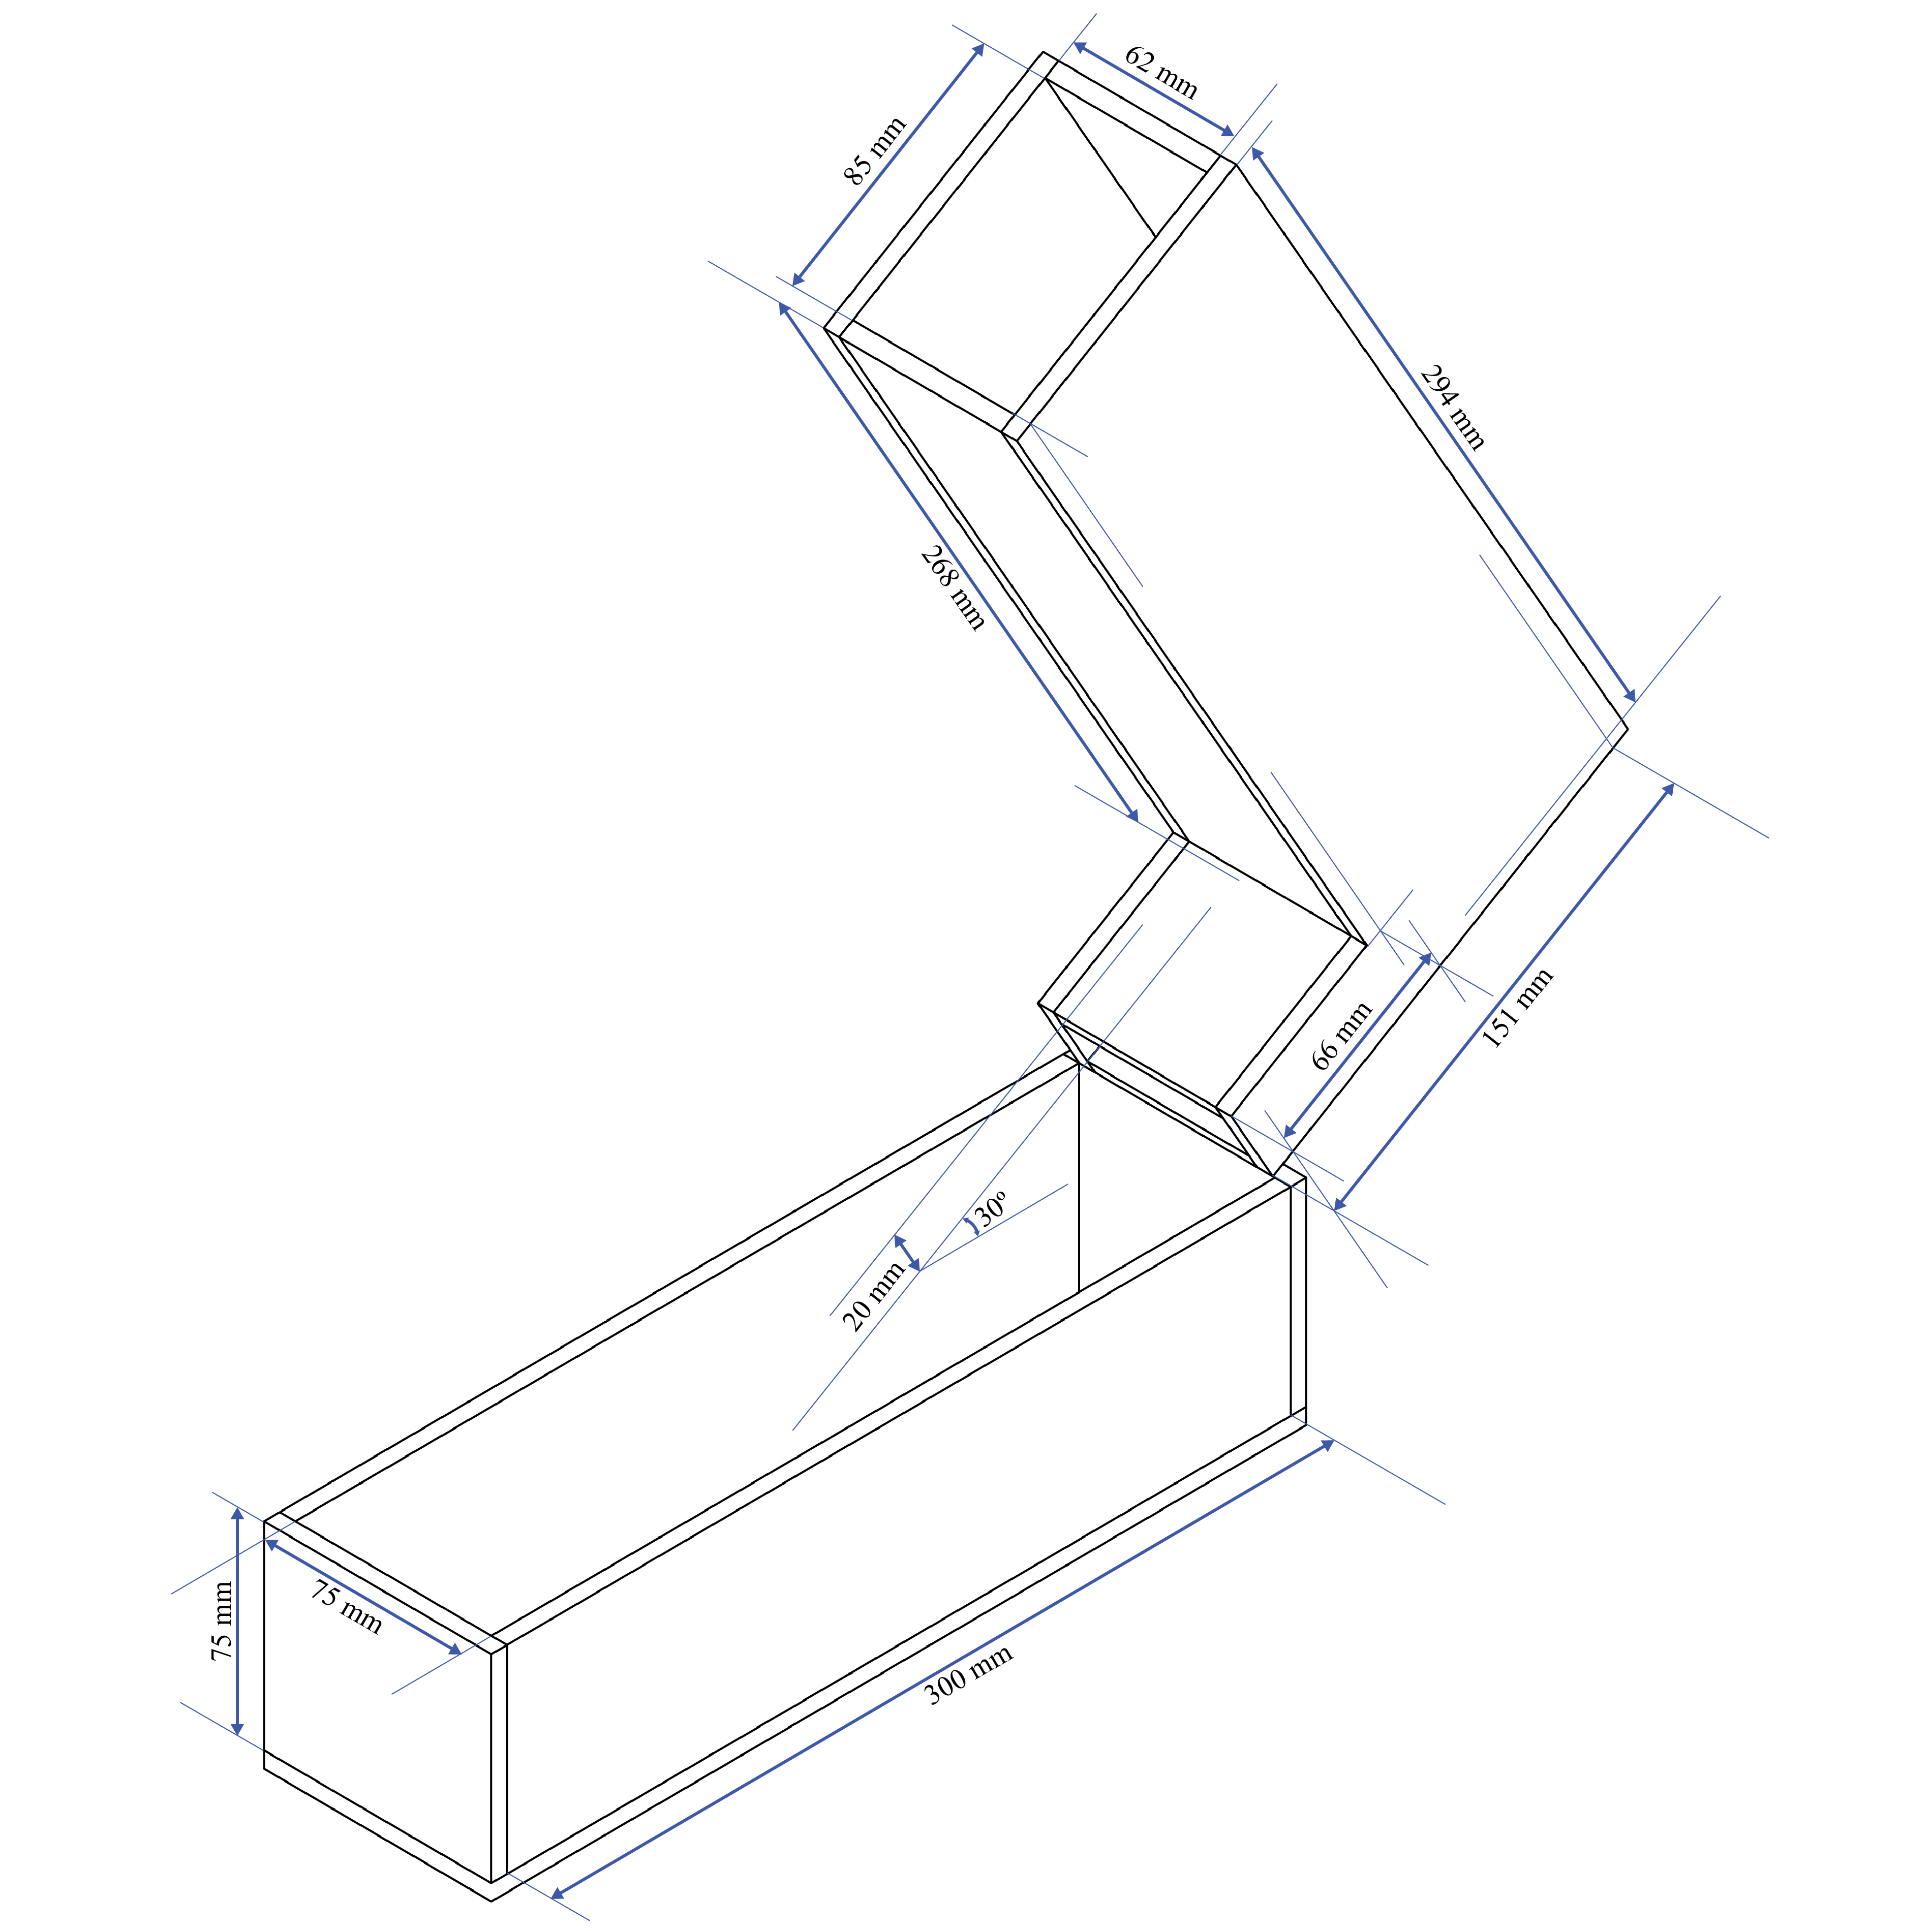
\includegraphics[width=0.7\textwidth]{Ilustraciones/SetUp Dimention.png}
    \caption{Caption.}
    \label{fig:setup_dim}
\end{figure}


\subsection{Optical setup}

\textcolor{blue}{Redaccion revisada}

\textcolor{red}{EN ESTA SECCION FALTA PONER MODELO DE LAS CAMARAS (CAM 1 A 3 MISMO MODELO) CAM 4 OTRO MODELO.}

Four high speed cameras record the flow, as Fig. \ref{fig:setup} shows, all fitted with $24$~mm $f/1.8$ lenses. The wide aperture allows short exposure times and reduces motion blur, at the cost of a reduced depth of field, which is acceptable because the planar laser sheet of the PIV and the narrow measurement volume of the PTV ensure that only features within the focal plane contribute to the measurement. Camera 1 covers the bend of the L-shape, cameras 2 and 3 cover the beam with a small overlap that permits the two fields to be reconstructed into one, and camera 4 is placed at the L-shape outlet, where the flow is fastest, at a higher frame rate and a finer scale factor. Table \ref{tab:cameras_specs} lists the operating parameters of each.

\begin{figure}[htbp]
    \centering
    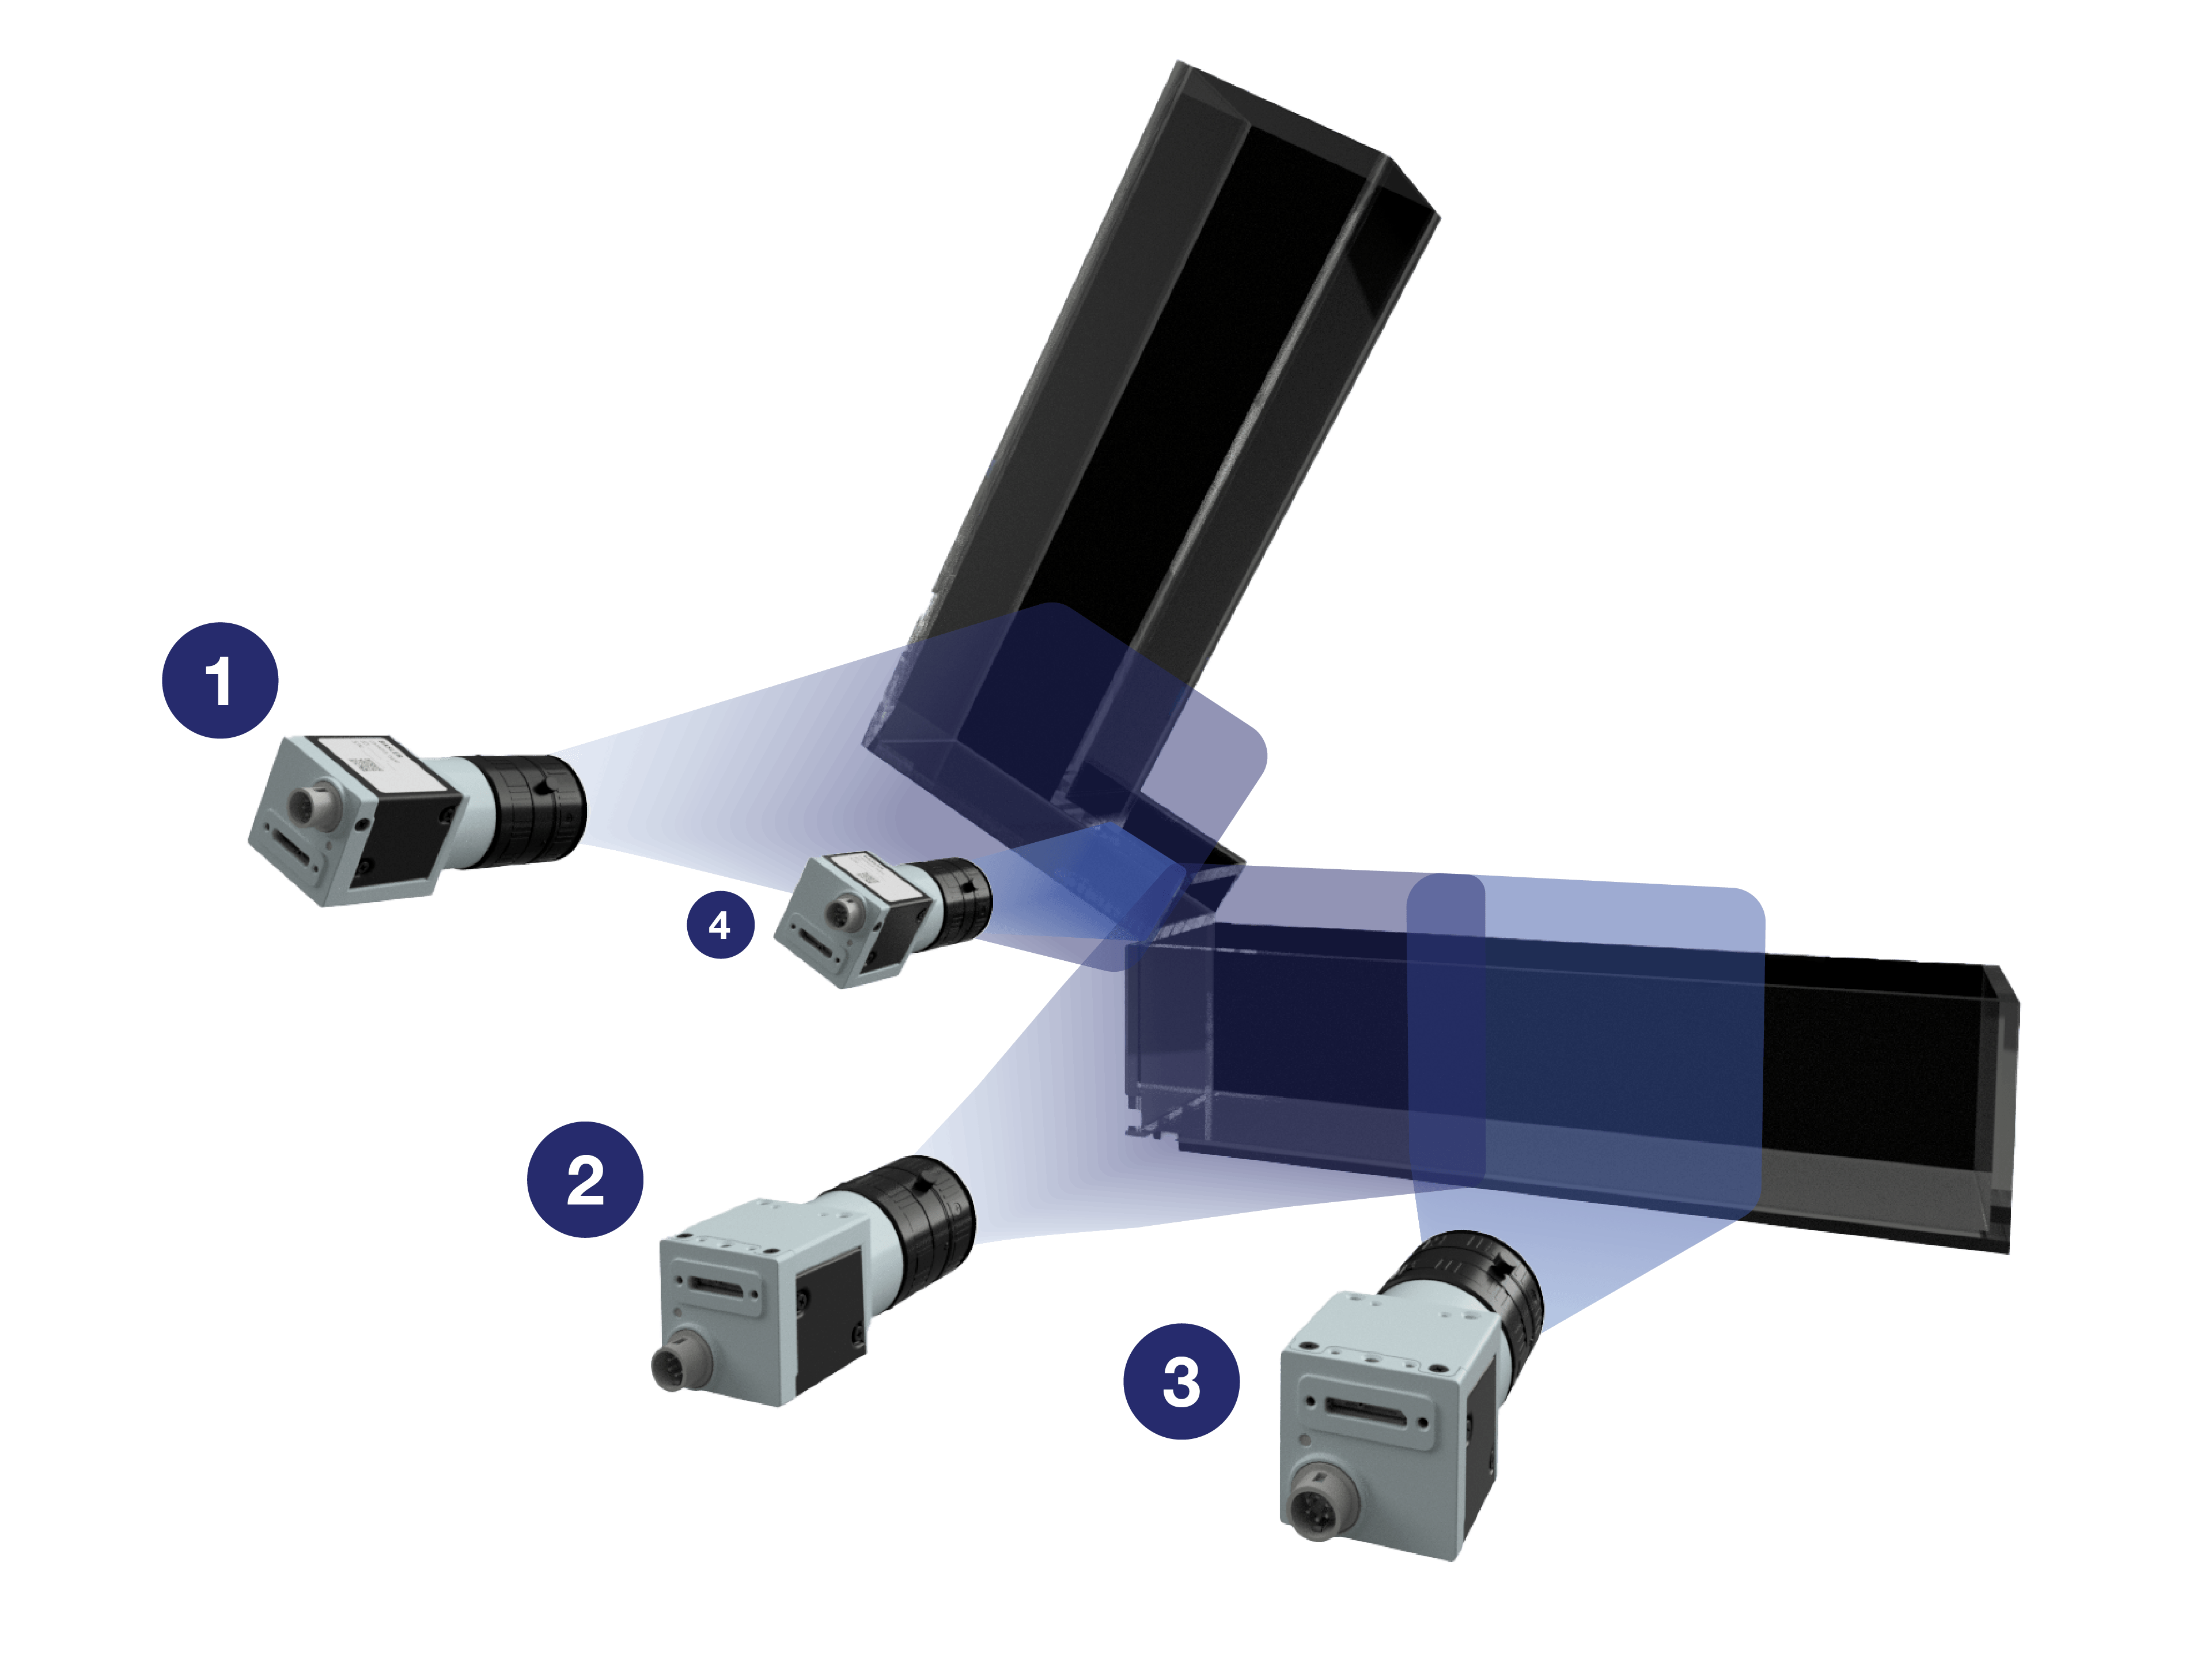
\includegraphics[width=0.7\textwidth]{Ilustraciones/SetUp Simple.png}
    \caption{Caption.}
    \label{fig:setup}   
\end{figure}

\begin{table}[htb]
\centering
\caption{Camera specifications and operating parameters.}
\label{tab:cameras_specs}
\begin{tabular}{
    c
    S[table-format=3.0]
    c
    S[table-format=1.4]
}
\toprule
\textbf{Camera} & {\textbf{Frame Rate}} & \textbf{Resolution} & {\textbf{Scale Factor}} \\
 & {\textbf{(fps)}} & \textbf{(pixels)} & {\textbf{(mm/px)}} \\
\midrule
1 & 220 & 1024 $\times$ 1024 & 0.1250 \\
2 & 220 & 1024 $\times$ 1024 & 0.1282 \\
3 & 220 & 1024 $\times$ 1024 & 0.1282 \\
4 & 660 & 384  $\times$ 384  & 0.0935 \\
\bottomrule
\end{tabular}
\end{table}

Because the analysis pairs the fluid and fiber fields at a common instant, the cameras are synchronized in hardware rather than by software timestamp. An external trigger drives the exposure of every camera and the signals are aligned on an oscilloscope, so that a given frame index corresponds to the same physical instant across all views. This is the condition under which the velocity field measured by one camera and the fiber state measured by another may be compared at the same point in time.

The scale factors of Table \ref{tab:cameras_specs} fix the resolution at which a fiber is seen, and the uncertainty of every quantity reported here descends from them. At $0.125$~mm~px$^{-1}$ a fiber of $13$~mm length and $0.2$~mm diameter projects onto approximately $104$~px along its axis and $1.6$~px across it. The fiber is therefore well resolved in length and barely resolved in width, which makes its orientation recoverable to a fraction of a degree while making its detection sensitive to illumination, and it is the reason the detection stage of Section~[REF] is treated as a measurement problem rather than as a preprocessing step. \textcolor{red}{ESTA ULTIMA AFIRMACION DEPENDE MUCHO DE COMO SE PLANTEA LA SECCION DE PTV}

\textcolor{red}{Una opcion de reemplazo de este ultimo parrafo es:}

\textcolor{olive}{
The fiber is therefore well resolved in length and barely resolved in width, which makes its orientation recoverable to a fraction of a degree while making its detection sensitive to illumination, and it is the origin of the orientation-dependent detection bias quantified in Section~\ref{sec:framework_uncertainty}.
}

\subsection{Transparent viscoplastic analogue}
\label{sec:analogue}

\textcolor{blue}{Redaccion revisada}

Fresh UHPC is opaque, and fibers travelling inside it cannot be seen at all. Carbopol, a crosslinked polyacrylic acid gel combining a yield stress with a shear-thinning post-yield response, replaces the cementitious matrix as the working fluid while allowing light to pass through it [CITAR]. The property the two matrices are required to share is the yield stress, since it is the yield stress alone that divides a casting into a moving sheared region and a rigid unyielded one, and it is that division which fixes how unevenly the strain is delivered to the fibers.

The curvature of the flow curve beyond yielding is not a settled property of fresh UHPC, having been reported as shear-thinning at the shear rates encountered during placement [CITAR] and as shear-thickening in mixes with a high content of fine powder [CITAR]. The shear-thinning response of Carbopol is therefore adopted here as a property of the working fluid, and is not asserted as a property the cementitious casting is thereby known to share.

Two concentrations of Carbopol Ultrez~10 were prepared, $0.2\%$ and $0.5\%$ by weight, differing in yield stress by approximately a factor of two. The pair was chosen for the contrast it supplies rather than for either value on its own, since the kinematics of a casting are governed by the yield stress and a model of it is tested not by reproducing a single flow but by reproducing the change a flow undergoes when that property is altered.

Each batch was prepared to a nominal volume of $2$~L. Deionized water was measured first and its initial pH verified to be approximately $7.0$, after which the corresponding mass of Carbopol powder was added gradually over one minute under mechanical stirring at $150$~rpm, and stirring was maintained for one hour to ensure complete and homogeneous dispersion of the polymer. The pH was then measured at five points across the mixture, a first dose of $1$~M NaOH was added, and the mixture was stirred for thirty minutes; a second dose followed, with a further thirty minutes of stirring, and the pH was measured again at five new points to confirm that the mean value fell within the accepted range. Table~\ref{tab:carbopol_recipe} gives the quantities for each formulation, and the pH recorded at each stage of the protocol for every batch of the campaign is given in the supplementary material.

\begin{table}[htb]
\centering
\caption{Preparation parameters for the two Carbopol Ultrez 10 formulations. The NaOH additions are sequential: the first dose initiates gelation and the second brings the mixture into the target pH range.}
\label{tab:carbopol_recipe}
\begin{tabular}{
    l
    S[table-format=4.0]
    S[table-format=2.1]
    S[table-format=2.0]
    S[table-format=2.0]
    c
}
\toprule
\textbf{Car} &
  \multicolumn{1}{c}{\makecell{Water \\ (mL)}} &
  \multicolumn{1}{c}{\makecell{Carbopol \\ (g)}} &
  \multicolumn{1}{c}{\makecell{NaOH$_1$ \\ (mL)}} &
  \multicolumn{1}{c}{\makecell{NaOH$_2$ \\ (mL)}} &
  \makecell{Target \\ pH} \\
\midrule
0.2\% & 1996 &  4.0 & 26 &  3 & 6.8--7.2 \\
0.5\% & 1990 & 10.0 & 70 & 20 & 6.8--7.2 \\
\bottomrule
\end{tabular}
\end{table}

The resulting gel was stored sealed at $20\,^\circ$C for twenty-four hours to complete hydration and stabilize its structure, and was then centrifuged at $2000$~rpm and $20\,^\circ$C for ten minutes to remove entrapped air, yielding an optically homogeneous gel. The centrifugation is not cosmetic: an elongated bubble in a translucent gel presents to the detector an object of the same aspect ratio and comparable contrast as a fiber, and is a source of false detections that no amount of training can wholly eliminate. Each batch was used for at most two experimental runs, and approximately $198$~mL are lost during dispersion, neutralization, centrifugation and transfer, leaving a working suspension of $1.802$~L over which the fiber volume fractions of Section~\ref{sec:fibers} are computed.

The rheology follows the Herschel-Bulkley model,

\begin{equation}
    \tau = \tau_0 + K\,\dot{\gamma}^{\,n},
    \label{eq:herschel_bulkley}
\end{equation}

in which $\tau_0$ is the yield stress, $K$ the consistency index and $n$ the flow index, and whose determination is complicated by wall slip. A thin polymer-depleted layer forms against smooth surfaces and allows the gel to slide before it yields in bulk, so that rotational rheometry on smooth walls systematically underestimates the yield stress of Carbopol suspensions [CITAR]. To obtain a slip-free estimate, $\tau_0$ was determined from the geometry of an arrested free surface flow rather than from rotational rheometry [CITAR]. When a yield-stress fluid spreads under gravity it comes to rest once the gravitational driving stress can no longer overcome the yield resistance, so the shape of the arrested deposit encodes $\tau_0$ directly and the measurement is made on the bulk material rather than at a wall. Applying the thin film lubrication balance to the arrested layer [CITAR] gives

\begin{equation}
    \tau_0 = \tfrac{1}{2}\,\rho\,g\,h_{\max}\tan\theta_\infty,
    \label{eq:arrested_deposit}
\end{equation}

with $\rho$ the fluid density, $g$ the gravitational acceleration, $h_{\max}$ the maximum height of the arrested fluid and $\theta_\infty$ the inclination of the free surface at rest, the prefactor following from the balance between the gravitational driving stress and the yield resistance integrated over the depth of the layer.

With $\tau_0$ fixed by this route, the consistency index $K$ and the flow index $n$ were obtained by refitting steady state flow curve data while holding $\tau_0$ at its slip-free value, so that the shear-thinning branch is captured without reintroducing the bias associated with wall slip. Table~\ref{tab:carbopol_rheology} collects the resulting parameters. The flow index below unity in both cases confirms the shear-thinning character of the two gels, while the higher yield stress and consistency of the $0.5\%$ formulation reflect its denser polymer network.

\begin{table}[htb]
\centering
\caption{Herschel-Bulkley parameters for the two Carbopol Ultrez 10 formulations. The yield stress $\tau_0$ was determined from the arrested free-surface deposit to avoid wall-slip underestimation; the consistency index $K$ and flow index $n$ were refitted from flow-curve data with $\tau_0$ held fixed. The critical shear rate $\dot{\gamma}_c = (\tau_0/K)^{1/n}$ separates the yield-dominated from the viscous-dominated response.}
\label{tab:carbopol_rheology}
\begin{tabular}{
    l
    S[table-format=2.1]
    S[table-format=2.2]
    S[table-format=1.3]
    S[table-format=2.1]
}
\toprule
\textbf{Car} & 
  \multicolumn{1}{c}{\makecell{$\tau_0$ \\ (Pa)}} & 
  \multicolumn{1}{c}{\makecell{$K$ \\ (Pa$\cdot$s$^n$)}} & 
  \multicolumn{1}{c}{\makecell{$n$ \\ (--)}} & 
  \multicolumn{1}{c}{\makecell{$\dot{\gamma}_c$ \\ (s$^{-1}$)}} \\
\midrule
0.2\% & 40.6 & 7.70  & 0.532 & 22.8 \\
0.5\% & 84.0 & 23.96 & 0.442 & 17.1 \\
\bottomrule
\end{tabular}
\end{table}

The critical shear rate $\dot{\gamma}_c = (\tau_0/K)^{1/n}$ deserves particular attention, because it locates the flow with respect to the mechanism on which this work rests. Below it, of the order of $20$~s$^{-1}$ in both formulations, the local stress remains close to $\tau_0$ and the material translates as a near-plug without deforming; above it the power law term dominates and the material shears. The deformation delivered to a fiber is therefore set by whether the region it crosses lies above or below this rate, and not by the distance it travels.

\subsection{Fibers and concentration regimes}
\textcolor{blue}{Redaccion revisada}

The fibers are straight steel fibers of $13$~mm length and $0.2$~mm diameter, giving an aspect ratio $r_f = 65$, commercially supplied for fiber reinforced concrete [CITAR]. The aspect ratio fixes the boundaries of the concentration regimes: the dilute limit at $\phi_{sd} = r_f^{-2} = 0.024\%$ by volume, below which the fibers do not interact, and the concentrated limit at $\phi_c = r_f^{-1} = 1.54\%$, above which they are in permanent contact. The semi-dilute regime lies between them, and it is the regime in which the interaction term of Equation~\eqref{eq:advani_tucker} is the appropriate description.


The aspect ratio fixes the boundaries of the concentration regimes through the mean spacing between neighboring fibers. Below a volume fraction at which a fiber can rotate freely through a full revolution without encountering another, the suspension is dilute and the interaction term of Equation~\eqref{eq:advani_tucker} vanishes; above a volume fraction at which the fibers are in permanent contact, the encounters cease to be uncorrelated events and the rotary-diffusion representation ceases to apply [CITAR]. The two bounds follow from $r_f$ alone,

\begin{equation}
    \phi_{sd} = r_f^{-2}, \qquad \phi_{c} = r_f^{-1},
    \label{eq:regime_limits}
\end{equation}

giving $\phi_{sd} = 0.024\%$ and $\phi_c = 1.54\%$ by volume for the fibers used here. The semi-dilute regime lies between them, and it is the regime in which the interaction term is the appropriate description: the fibers are close enough to disturb one another and not so close as to be permanently in contact.

Three dosages were tested together with a fiber-free control, placed at $0.72$, $1.48$ and $2.92$ times the dilute limit, so that the design brackets the onset of the interaction mechanism rather than probing a single point of it. Fibers were counted by weighing, using the manufacturer's numerical density as the conversion factor and a balance whose resolution is finer than the mass of a single fiber, approximately $3.5$~mg \textcolor{red}{REVISAR ESTE VALOR}, by at least an order of magnitude. Table~\ref{tab:fiber_concentrations} locates these dosages against the regime boundaries of Equation~\eqref{eq:regime_limits} and against a practical UHPC mix.

The distance the table reveals is the context for a result that recurs throughout this work. A practical mix carries $1$ to $2\%$ of fibers by volume, that is $0.65$ to $1.30$ times the concentrated limit, so its fibers are in near-permanent contact; the dosages reached here are one to two orders of magnitude below that, at the lower edge of the semi-dilute regime. The constraint is optical rather than a matter of design. A suspension dense enough to reproduce a real element is one in which the fibers occlude one another and can no longer be resolved individually, so raising the dosage to close the gap would defeat the measurement itself. Its consequence for what follows is definite and works in one direction only: the interactions are the weakest they can be while remaining nonzero, so any effect recovered here is a lower bound on what a practical mix would produce.

\begin{table}[htb]
\centering
\footnotesize
\caption{Fiber dosages of the experimental campaign, set against the boundaries of the concentration regimes and against the dosages of a real UHPC mix. The number in the L-shape is the subset deposited within the device at a fill height of $22.4$~mm, about $73\%$ of each batch, and is informative only; the volume fractions and their ratios are computed over the full working suspension of $1.802$~L, from the nominal fiber volume of $0.408$~mm$^{3}$. Two regime boundaries follow from the aspect ratio $r_f = 65$: the dilute limit $\phi_{sd} = r_f^{-2}$, below which the fibers do not interact, and the concentrated limit $\phi_{c} = r_f^{-1}$, above which they are in permanent contact; the semi-dilute regime lies between them. The campaign occupies the lower edge of that regime, while a real UHPC mix sits at or above its upper edge. Reference rows are not tested conditions.}
\label{tab:fiber_concentrations}
\setlength{\tabcolsep}{4pt}
\begin{tabular}{
    l
    S[table-format=5.0]
    S[table-format=2.3]
    S[table-format=1.3]
    S[table-format=5.0]
    S[table-format=2.3]
    S[table-format=1.3]
}
\toprule
& \multicolumn{1}{c}{\makecell{\textbf{N° of} \\ \textbf{Fibers}}}
& \multicolumn{1}{c}{\makecell{\textbf{Weight} \\ \textbf{Fract. (\%)}}}
& \multicolumn{1}{c}{\makecell{\textbf{Volume} \\ \textbf{Fract. $\phi$ (\%)}}}
& \multicolumn{1}{c}{\makecell{\textbf{N° in} \\ \textbf{L-shape}}}
& \multicolumn{1}{c}{\makecell{\textbf{$\phi/\phi_{sd}$} \\ \textbf{(--)}}}
& \multicolumn{1}{c}{\makecell{\textbf{$\phi/\phi_{c}$} \\ \textbf{(--)}}} \\
\midrule
\multicolumn{7}{l}{\textit{Experimental campaign}} \\
\midrule
$N_0$ &    0 & 0.000 & 0.000 &    0 & 0.000 & 0.000 \\
$N_1$ &  750 & 0.140 & 0.017 &  547 & 0.720 & 0.011 \\
$N_2$ & 1500 & 0.270 & 0.035 & 1094 & 1.480 & 0.023 \\
$N_3$ & 3000 & 0.500 & 0.069 & 2188 & 2.920 & 0.045 \\
\midrule
\multicolumn{7}{l}{\textit{Regime boundaries} ($r_f = 65$)} \\
\midrule
Dilute limit $\phi_{sd} = r_f^{-2}$      &  1023 & 0.185 & 0.024 &   746 &  1.000 & 0.015 \\
Concentrated limit $\phi_{c} = r_f^{-1}$ & 66525 & 12.000 & 1.538 & 48509 & 65.000 & 1.000 \\
\midrule
\multicolumn{7}{l}{\textit{Real UHPC mix}} \\
\midrule
UHPC ($1\%$ vol.) & 43241 & 7.800 & 1.000 & 31531 & 42.300 & 0.650 \\
UHPC ($2\%$ vol.) & 86482 & 15.600 & 2.000 & 63062 & 84.500 & 1.300 \\
\bottomrule
\end{tabular}
\end{table}

\textcolor{red}{LLAMAR A LA FIGURA EN EL TEXTO}

\begin{figure}[htbp]
    \centering
    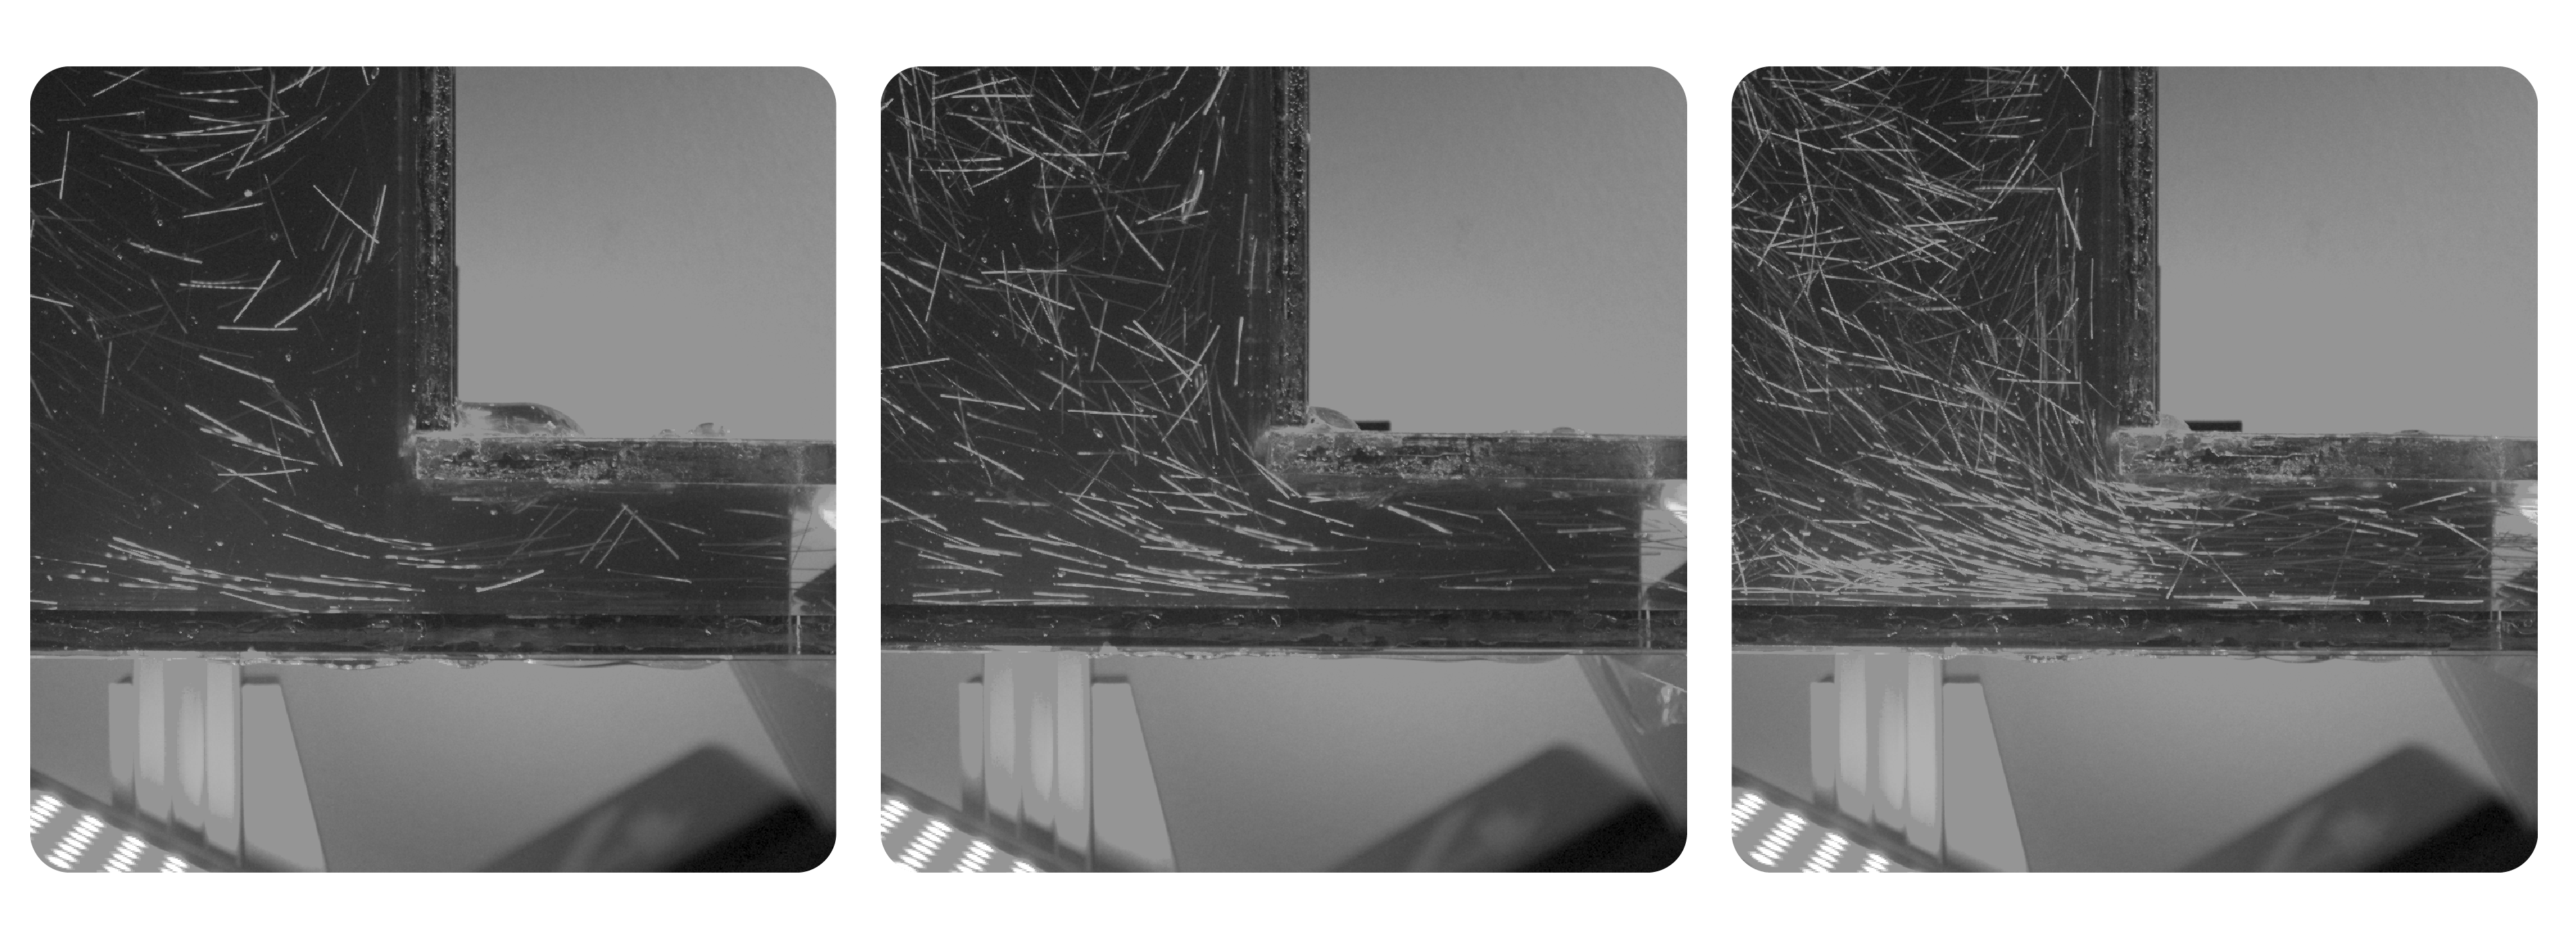
\includegraphics[width=0.9\textwidth]{Ilustraciones/ValidationTakes.png}
    \caption{Caption.}
    \label{fig:validation_takes}
\end{figure}

\subsection{Experimental campaign}
\textcolor{blue}{Redaccion revisada}

The campaign varies one factor at a time. The geometry and the filling procedure are held fixed, and within each series the rheology is fixed as well, so that the fiber content is the only quantity changing between runs and any difference in the orientation it produces is attributable to it. Two series are conducted, one in each Carbopol formulation, supplying the contrast in yield stress. Each formulation and dosage combination was replicated with two independently prepared batches, so that the batch to batch variability of the gel is separated from the effect of the fibers, and every batch supplies two acquisitions. In the runs carrying fibers the two acquisitions are a PTV followed by a PIV: the fiber dynamics are recorded first, tracers are then seeded into the same gel, and the pour is repeated, so that the velocity field and the fiber orientations are obtained on the same batch and under identical conditions. In the fiber-free runs both acquisitions are PIV.

\subsection{Non-Intrusive Techniques}

\textcolor{blue}{Redaccion revisada}

The role of the PIV is to supply the independent variable of the saturation law. The velocity field is not the object of the measurement but the means of obtaining one: differentiated in space it gives the rate of deformation and the shear rate, and integrated along the trajectories it defines it gives Equation~\eqref{eq:accumulated_strain}. It is measured on every run and not only on the fiber-free ones, because a suspension carrying more fibers advances more slowly than one carrying fewer, so the strain against which an orientation is read must be the strain that same suspension delivered.

Where the PIV supplies the independent variable, the PTV supplies the dependent one. The orientations of the fibers detected within a region reduce to the order parameter of Equation~\eqref{eq:eta_1}, and the same rod tracked across successive frames yields in addition its angular velocity. Both are recovered from the same detections, and the detection stage is therefore treated as a measurement problem rather than as a preprocessing step. The reason is that the fibers a detector fails to find are not a random sample of the population: a rod inclined unfavorably with respect to the illumination returns less light to the camera than one inclined favorably, so a detection rate below unity biases the measured distribution toward the orientations that are easiest to see. The framework was developed and validated in a companion study [CITAR] and is summarized here.

\textcolor{red}{AQUI AJSTAR LA REDACCION SEGUN CUANTO SE PROFUNDICE EN EL PIV Y PTV EN LA SIGUIENTE SECCION, ADEMAS DE CITAR EL COMPANION STUDY Y TESIS}

\textcolor{red}{PROPUESTA:}

\textcolor{olive}{
% Reemplaza el segundo párrafo de III F
Where the PIV supplies the independent variable, the PTV supplies the dependent one. The orientations of the fibers detected within a region reduce to the order parameter of Equation~\eqref{eq:eta_1}, which is the quantity the saturation law predicts, and the same rod tracked across successive frames yields in addition its angular velocity. Both are recovered from the same detections. The framework was developed and validated in a companion study [CITAR], and Section~\ref{sec:framework_ptv} summarizes the elements of it on which the present measurements depend.
}

% ============================================================
\section{Analysis Framework}
\label{sec:framework}
% ============================================================

\textcolor{blue}{Redaccion revisada}

The saturation law of Section~\ref{sec:governing} relates two quantities, the strain a population of fibers has accumulated and the degree of alignment it has acquired, and neither is delivered directly by a camera. The first must be integrated from a velocity field along the path the material followed, and the second must be assembled from the orientations of fibers detected individually within a region. This section describes how both are recovered from the recorded images, the decisions that recovery requires, and the uncertainty each decision introduces. The two techniques are treated in turn, followed by the partition of the domain that makes a local reading possible, the integration that produces the independent variable, the reconstruction that establishes which fibers received it, and the uncertainty budget and statistical protocol under which the results of Section~[REF] are reported.

% ------------------------------------------------------------
\subsection{Velocity fields from PIV}
\label{sec:framework_piv}
% ------------------------------------------------------------

\textcolor{blue}{Redaccion revisada}

The velocity field is obtained by cross-correlation of tracer displacements between consecutive image pairs, using a multi-pass scheme in which the interrogation window is progressively refined [CITAR]. The final window size sets the spatial resolution of the field and was adapted to the flow each camera records: the views covering the fastest regions of the softer formulation retain a larger final window, since particles would otherwise leave a smaller one between the two frames of a pair, while the remaining configurations use a finer window consistent with their lower velocities. 

Two features of the flow place demands on the correlation that a steady flow would not, and the first is its transient character. The material accelerates as it enters the mold, reaches its maximum velocity at the bend, and decelerates as it spreads along the beam until it arrests, so a correlation interval appropriate to the first phase produces displacements too small to correlate in the last. The image sequence is therefore divided into temporal blocks with progressively increasing correlation intervals, short while the flow is fast and longer as it slows, so that the particle displacement between the two frames of a pair remains within the range the correlation can resolve throughout the filling.

\textcolor{red}{LLAMAR A LA FIGURA EN EL TEXTO}

\begin{figure}[htbp]
    \centering
    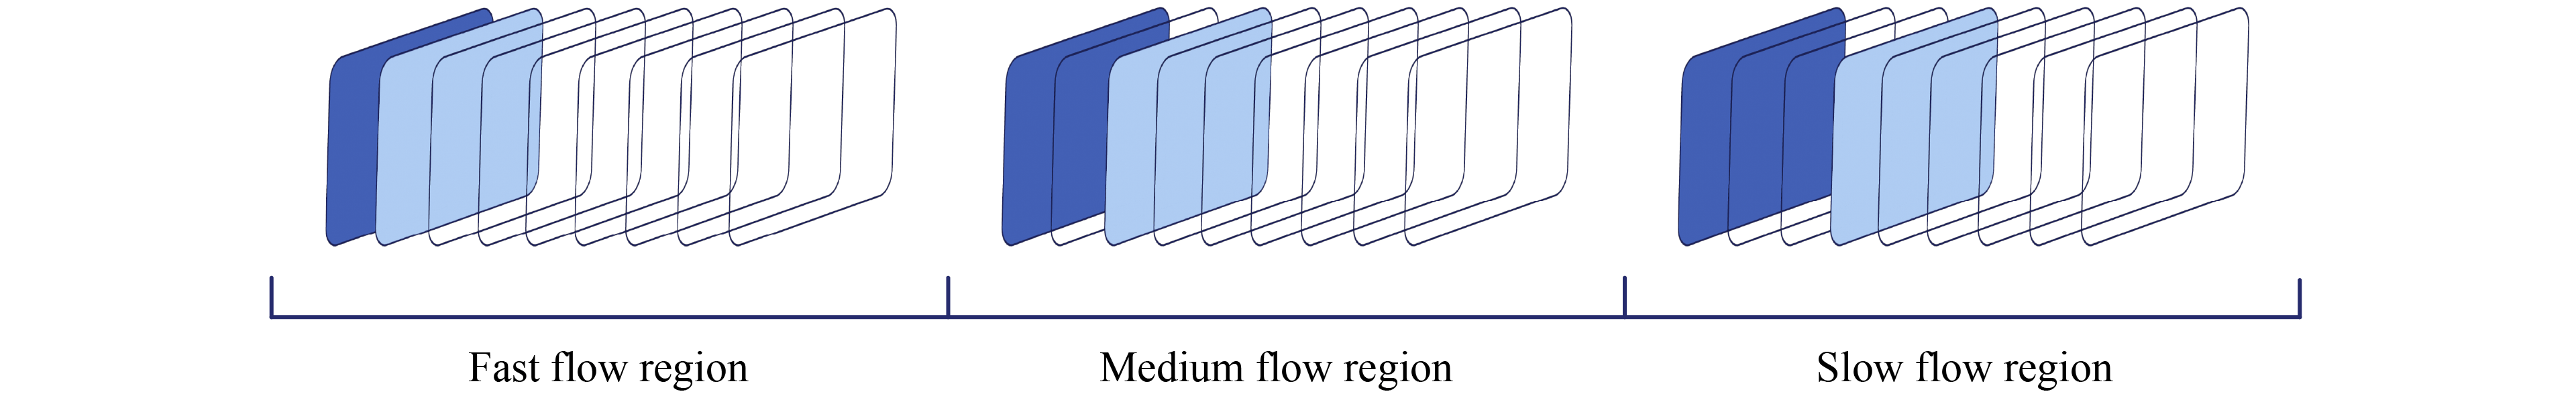
\includegraphics[width=1.0\textwidth]{Ilustraciones/PIV Blocks.png}
    \caption{Caption.}
    \label{fig:piv_block_structure}
\end{figure}

The block boundaries are not prescribed a priori but located from a validation diagnostic. Each vector is compared with the median of its $3\times3$ neighborhood through the normalized residual [CITAR],

\begin{equation}
    R_{i,j} = \frac{\left|\vec{V}_{i,j} - \vec{V}_m\right|}{r_m + \epsilon},
    \label{eq:uod}
\end{equation}

in which $\vec{V}_m$ is the median vector of the neighbors, $r_m$ the median of the absolute residuals within the neighborhood, and $\epsilon$ a small normalization factor accounting for measurement noise, and a vector is classified as spurious when $R_{i,j}$ exceeds a fixed threshold. This test evaluates the validity of a vector from local physical coherence rather than from global statistics, which is what makes it appropriate to a laminar flow carrying strong velocity gradients [CITAR]. The evolution of the fraction of spurious vectors is then used as the criterion that locates the block transitions: an abrupt rise in the failure rate indicates that the particle displacement has fallen below the level at which the correlation can be resolved, and triggers the transition to a longer interval.


The second feature is that the flow is viscoplastic, so the deformation is not distributed through the domain but confined to the sheared layers separating the plug from the walls, and the velocity gradient is therefore small over most of the field and large within a narrow band. Because the Reynolds number (\textcolor{red}{PONER NUMERO DE REYNOLDS PARA CAR 02 Y 05}) evaluated with the apparent viscosity at the characteristic shear rate of the bend remains below unity, the flow is laminar throughout, and intermediate frames between the analyzed pairs may be skipped without loss of information. This reduces the number of correlated pairs without altering the temporal resolution over the phases in which the field changes fastest.

\textcolor{red}{GENERAR MATERIAL SUPLEMENTARIO DE ESTA SECCION}

\textcolor{olive}{The window sequence adopted for every camera and formulation, together with the block structure and the sensitivity analysis from which both were fixed, is given in the supplementary material.}

% ------------------------------------------------------------
\subsection{Fiber detection and tracking}
\label{sec:framework_ptv}
% ------------------------------------------------------------

\textcolor{red}{REVISAR LA REDACCION DE ESTA SECCION YA QUE CAMBIARON VARIAS COSAS, ADEMAS, HAY QUE MENCIONAR QUE LOS ANALISIS DE SENSIBILIDAD Y ESTRUCTURA DE BLOQUES USADA ASI COMO REDUCCION DE COSTO COMPUTACIONAL SE ENCUENTRA EN EL MATERIAL SUPLEMENTARIO.}

The detection stage is treated here as a measurement problem rather than as a preprocessing step, and the reason is that the fibers a detector fails to find are not a random sample of the population. The steel fibers are specular reflectors, so a rod inclined unfavorably with respect to the illumination returns less light to the camera than one inclined favorably, as Fig.~\ref{fig:fiber_illumination} illustrates, and a detection rate below unity therefore biases the measured distribution toward the orientations that are easiest to see. Missing such a fiber removes a specific direction from the measured distribution rather than a random member from the count, which is a different kind of loss from a random one and must be bounded rather than assumed negligible. How this bias is quantified, and what the analysis requires of it, is set out in Section~\ref{sec:framework_uncertainty}.

\begin{figure}[htb]
    \centering
    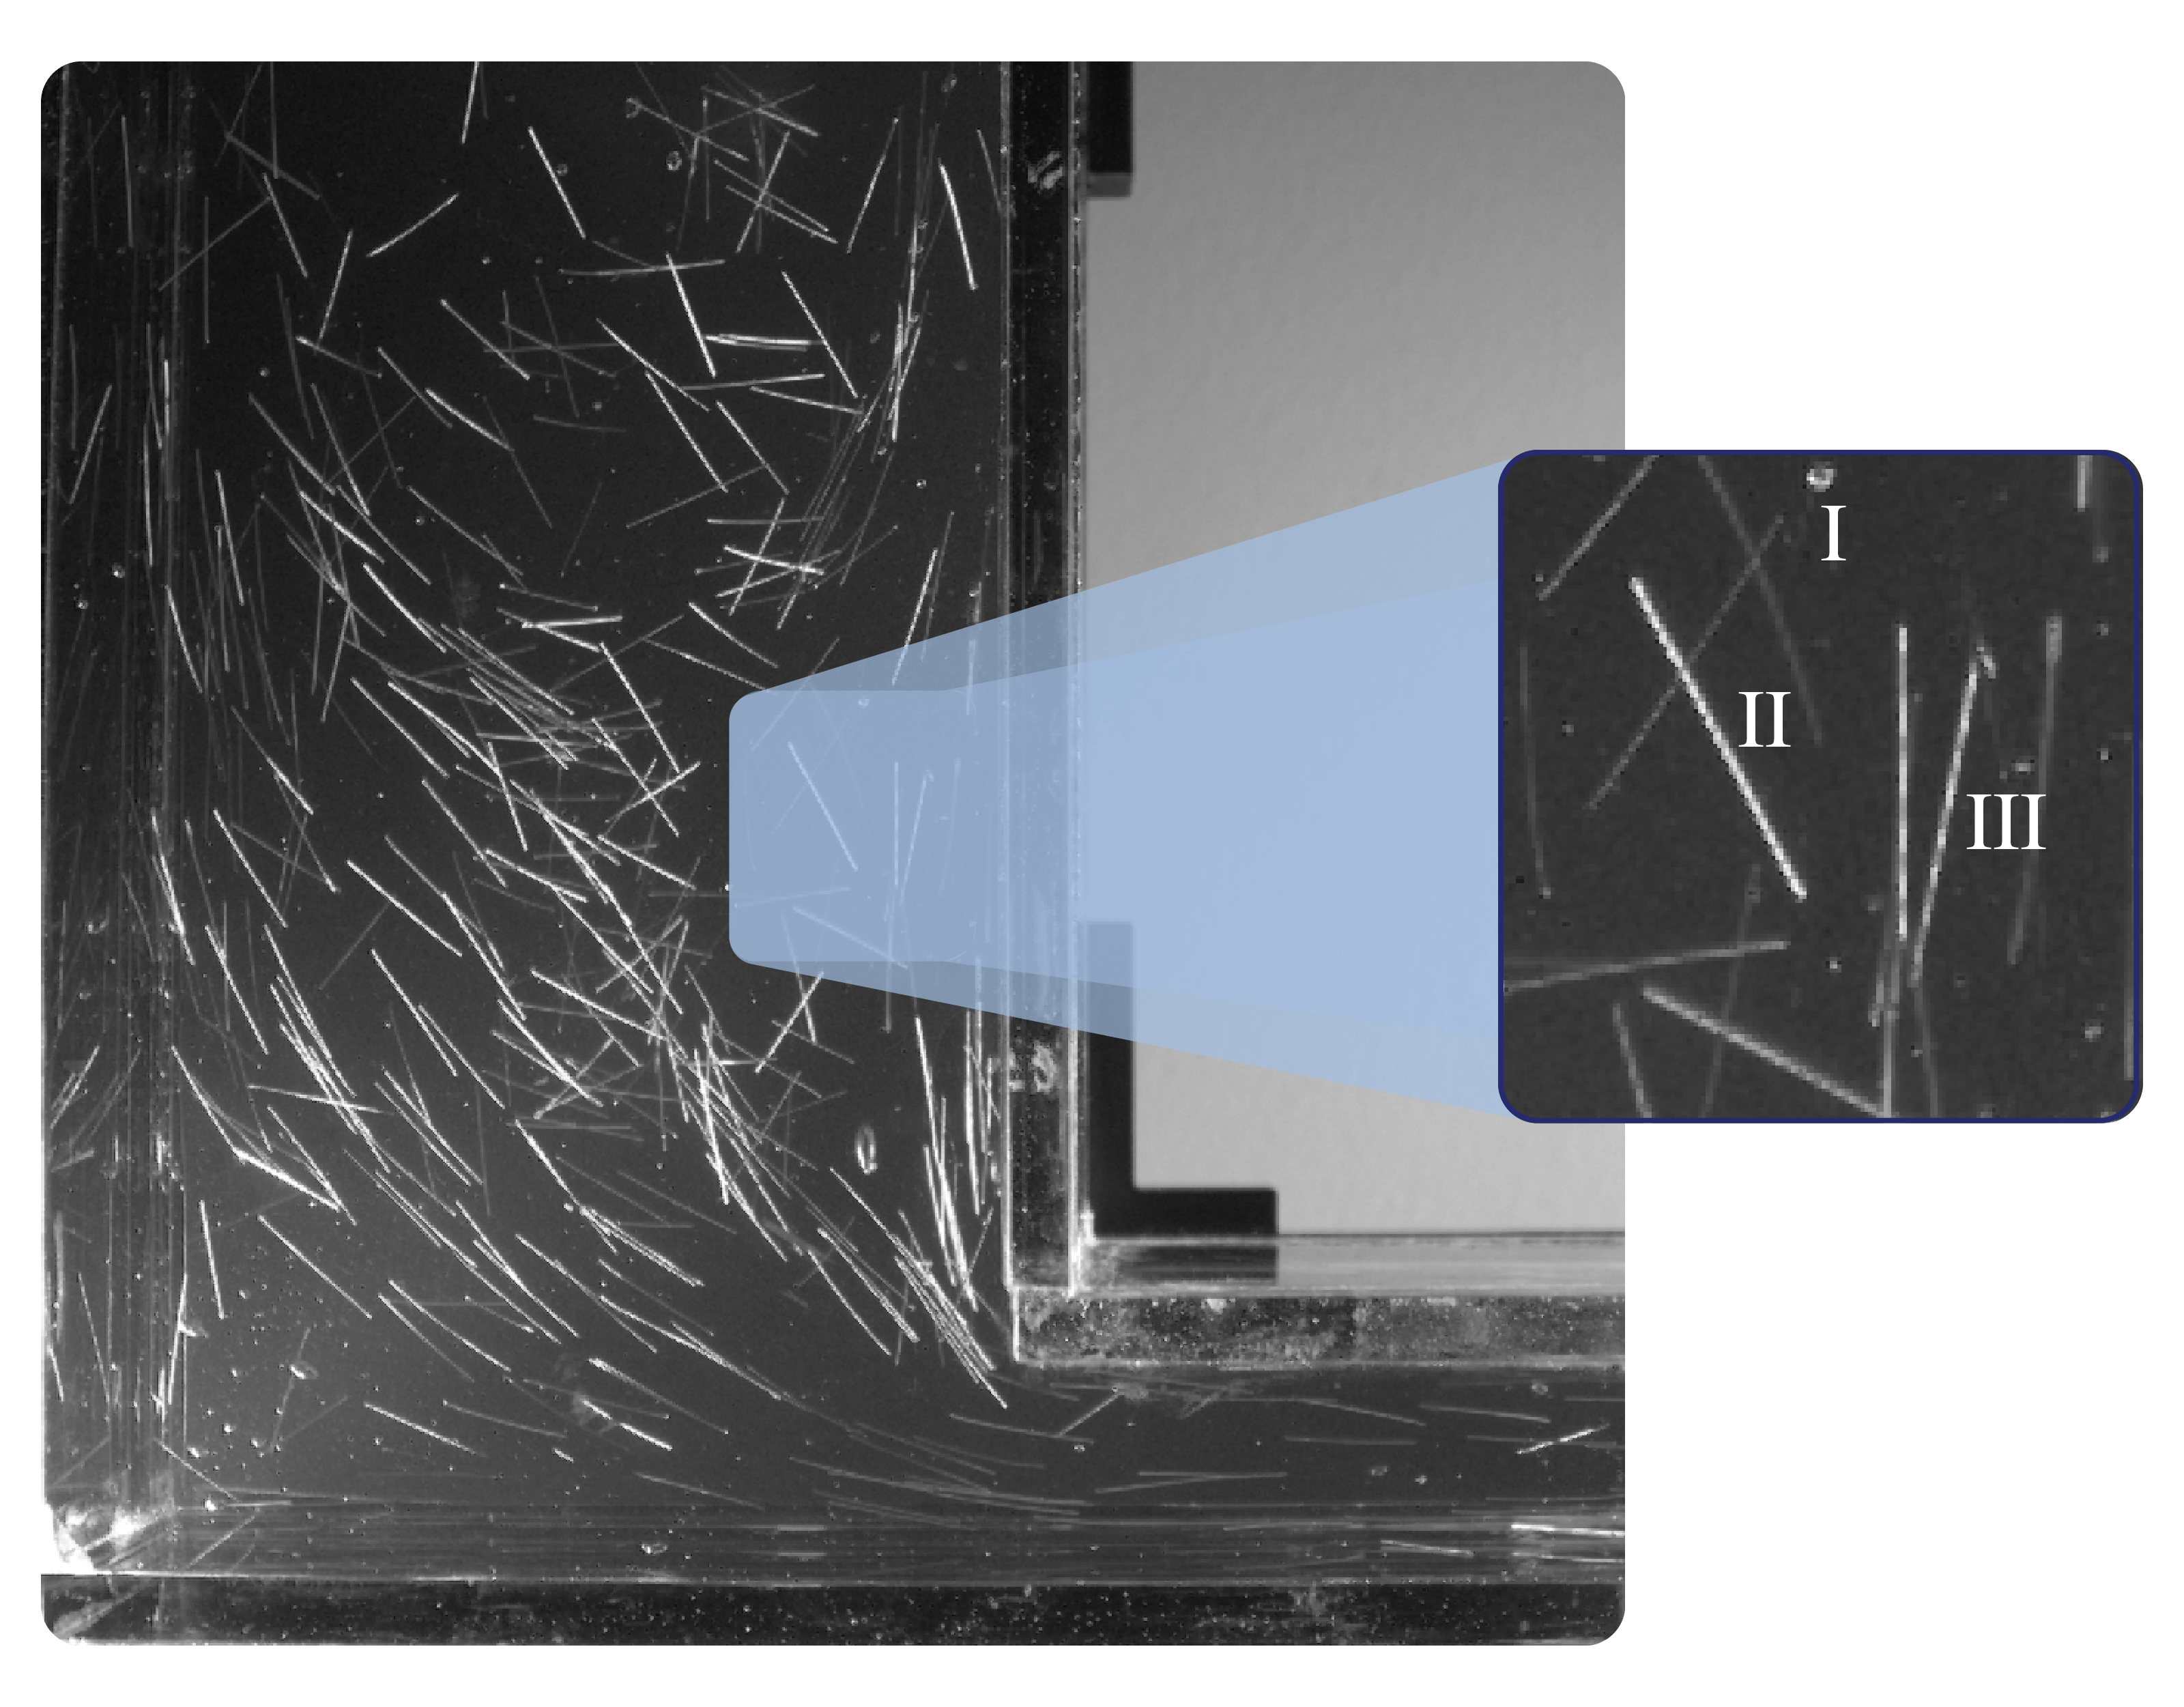
\includegraphics[width=0.6\textwidth]{Ilustraciones/NonUniformIlumination.png}
    \caption{Caption.}
    \label{fig:fiber_illumination}
\end{figure}

Detection is performed by an instance segmentation network fine tuned on a domain specific dataset of manually annotated frames, and association across frames combines a kinematic prediction of every established track, which supplies a constrained search region and carries a fiber through a frame in which the segmentation misses it, with a similarity match between the predictions and the detections falling within that region. The framework, its training, and its validation against a classical Hough transform baseline and an alternative promptable segmentation model are reported in a companion study [CITAR], where the network is shown to recover the large majority of the visible fibers at a low false detection rate. Two elements were developed for the present campaign and are described here, because the campaign reaches fiber loadings beyond those the original framework was validated against and a transient filling imposes a sampling constraint a steady sequence does not.

The first is the detection of fibers within dense clusters. The projected width of a fiber spans approximately two pixels, and the segmentation of adjacent, partially overlapping rods depends on that dimension, so at the highest dosages the field is upscaled by a factor of two before segmentation, raising the projected width to approximately four pixels, and is then divided into overlapping patches so that the network operates at the scale for which it was trained rather than on a downsampled view of the whole field. The detections are reassembled onto the original image through non maximum suppression, which resolves the duplicate predictions arising from the patch overlap. The training set was correspondingly extended with frames drawn from the densest runs, annotated in a model assisted loop in which an initial segmentation was verified and corrected by hand so that the annotations rest on human judgment and not on the predictions of the earlier detector, and a dedicated model was trained on a dataset processed through the same upscaling and tiling logic so that the training and inference distributions coincide. Fig.~\ref{fig:dense_detection} shows the procedure.

\begin{figure}[htb]
    \centering
    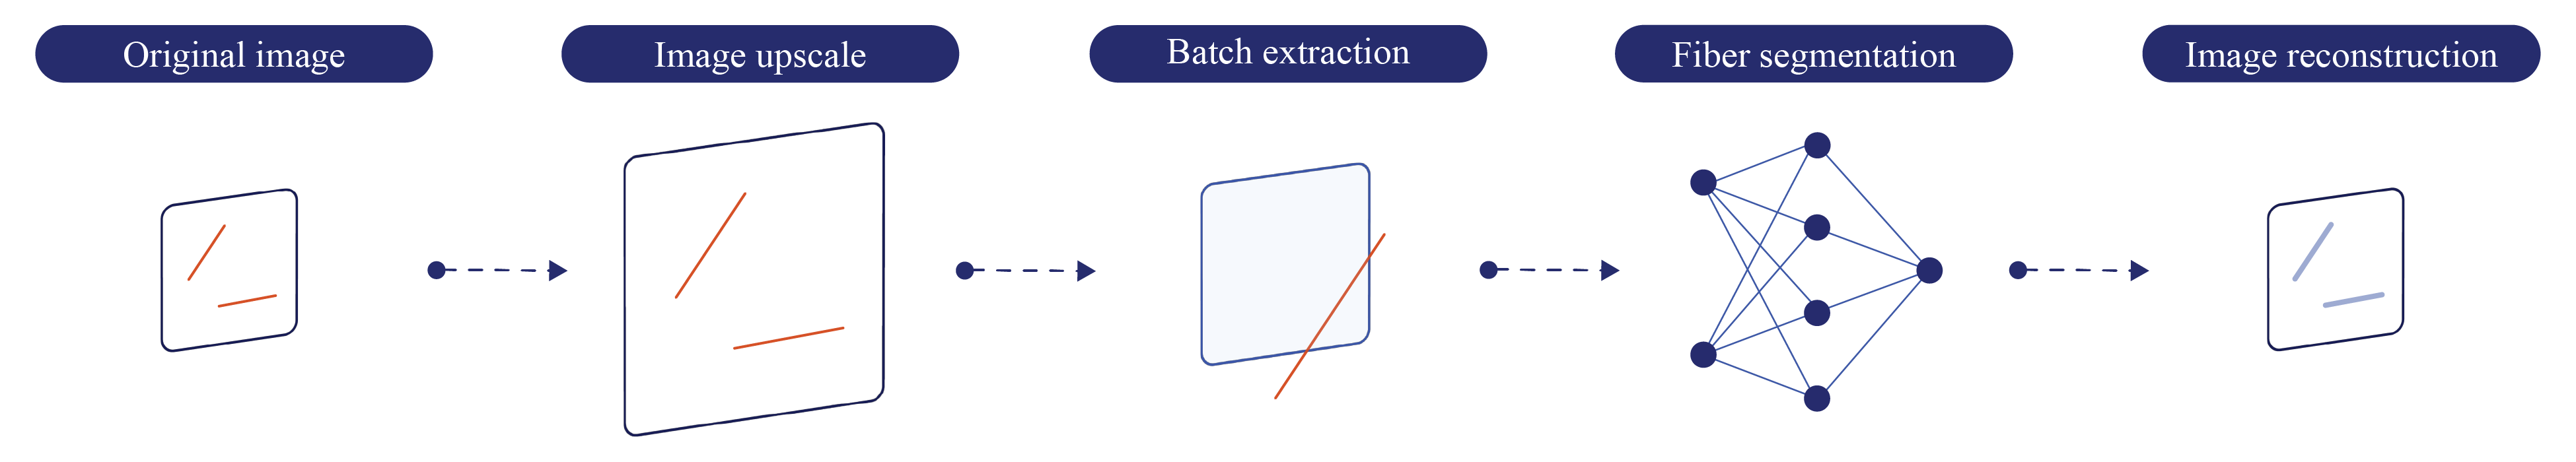
\includegraphics[width=1.0\textwidth]{Ilustraciones/FiberDetectionUpScale.png}
    \caption{Caption.}
    \label{fig:dense_detection}
\end{figure}

The second is the temporal sampling. A block structure analogous to that of the PIV governs it, although it means something different: the PIV correlates image pairs, so its blocks set the interval between the two frames of a pair, whereas the PTV analyzes each frame independently and then links the detections, so its blocks set how many frames are skipped between the frames that are analyzed. The interval is constrained from both sides, and more tightly here than in the PIV. Too long an interval lets a fiber travel beyond the search region between analyzed frames, so the track breaks and the trajectory is lost. Too short an interval reduces the displacement between analyzed frames toward the localization noise, so that the change in position carries less signal than the error in measuring it, and the angular velocity computed from it degrades. The block boundaries are therefore placed where the measured displacement distribution stays within both bounds, which is what minimizes the error on the angular velocity while reducing the number of frames segmented and with it the computational cost of the analysis. Fig.~\ref{fig:ptv_blocks} illustrates the structure; the intervals adopted for every camera and formulation, the displacement diagnostic from which each was fixed, and the resulting reduction in cost are given in the supplementary material.

\begin{figure}[htb]
    \centering
    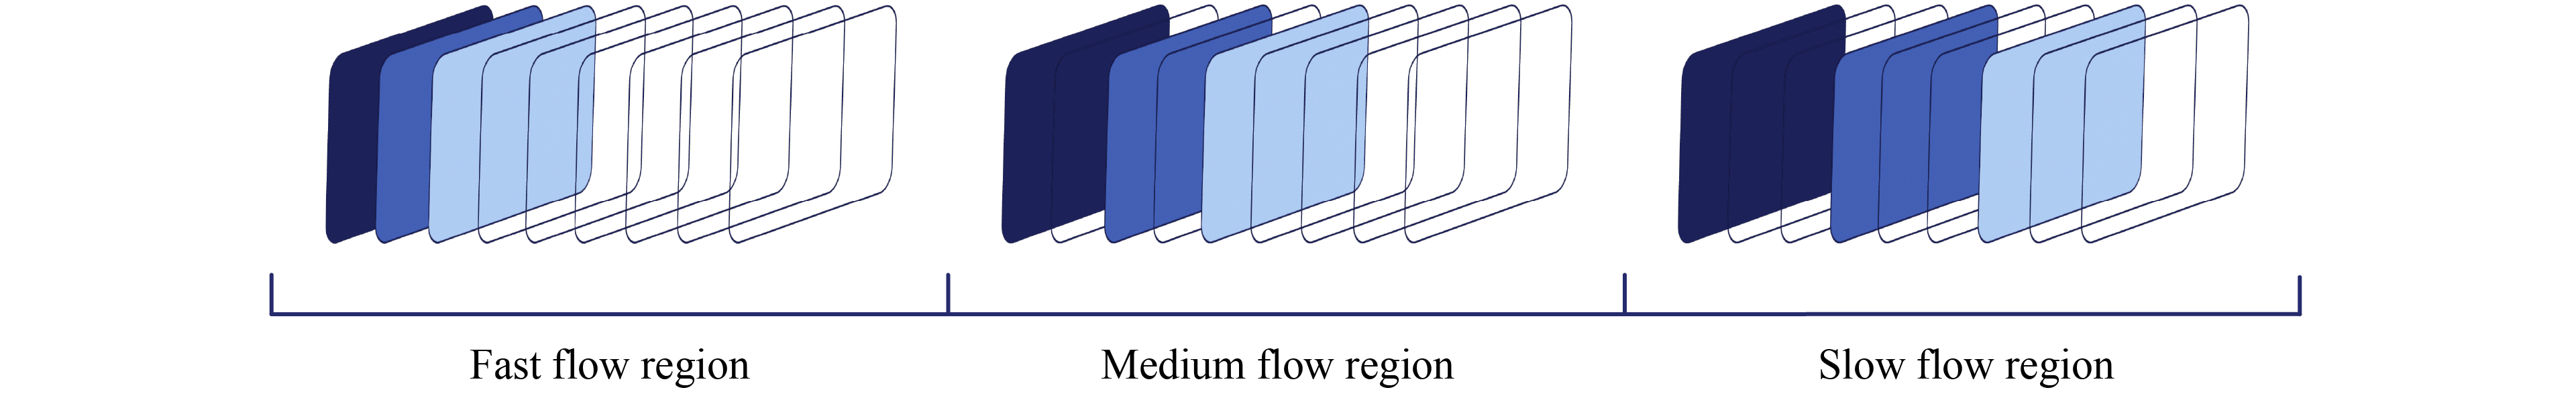
\includegraphics[width=1.0\textwidth]{Ilustraciones/PTV Blocks.png}
    \caption{Caption.}
    \label{fig:ptv_blocks}
\end{figure}

% ------------------------------------------------------------
\subsection{Spatial partition and flow stages}
\label{sec:framework_zones}
% ------------------------------------------------------------

\textcolor{blue}{Redaccion revisada}

Every quantity reported in this work is local, and the partition that makes it so is an instrument of the analysis rather than a convenience of presentation. A fiber accumulates strain unevenly along its path, so both the order parameter and the accumulated strain vary across the mold, and an average over the whole domain would conflate regions in which the material has been strongly deformed with regions in which it has barely deformed at all. The partition is what allows a single casting to supply a range of accumulated strain rather than a single value, and it is therefore the means through which the saturation law of Equation~\eqref{eq:saturation} can be traced at all.

The L-shape is divided into three zones following the sequence of flow conditions along the casting path: the vertical arm, where the flow is predominantly translational and the material advances largely as a plug; the elbow, where the flow turns through ninety degrees and both the deformation and the vorticity reach their maxima; and the outlet, where the flow passes from the L-shape into the beam. The beam is partitioned into a two by three grid of cells, with the lower row adjacent to the outlet. The partition is defined once and applied identically to every formulation and fiber dosage, so that a quantity measured in one condition is comparable with the same quantity measured in another.

Fig.~\ref{fig:zone_partition} shows the partition, drawn to the proportions of the mold so that the relative sizes of the zones are those they occupy in the experiment.

\begin{figure}[htbp]
    \centering
    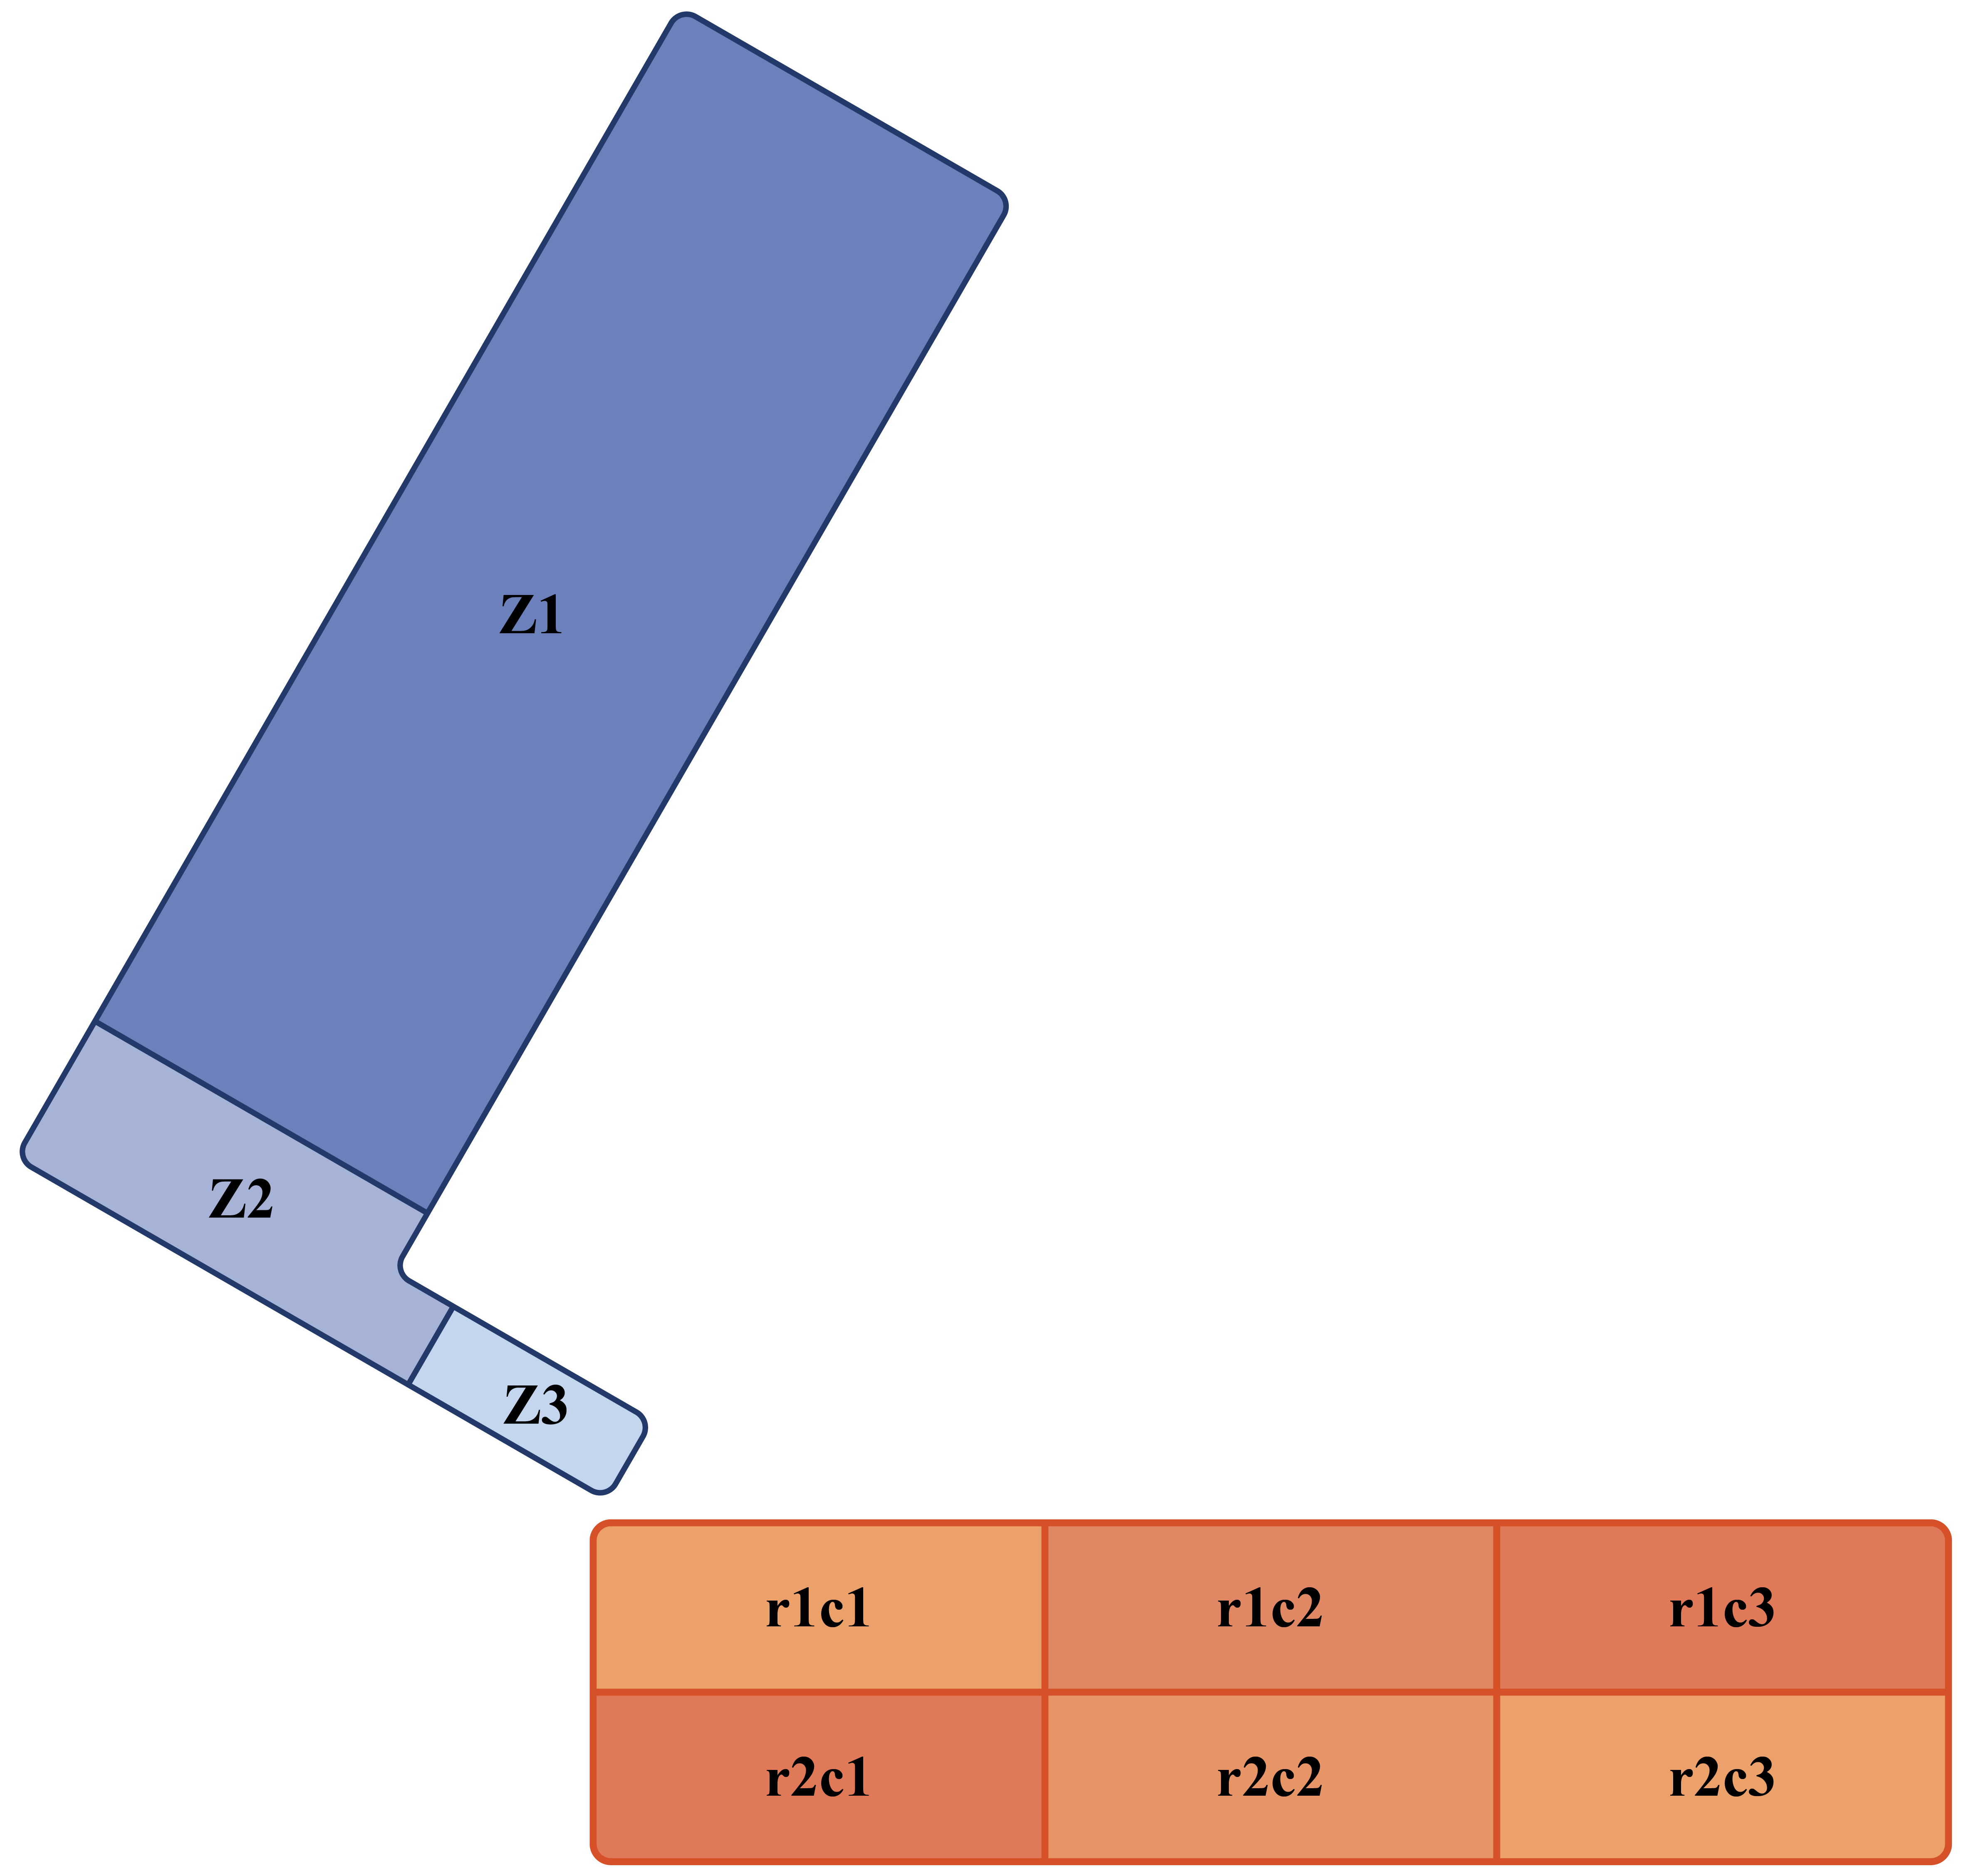
\includegraphics[width=0.5\textwidth]{Ilustraciones/zones.png}
    \caption{Spatial partition of the domain. The L-shape is divided into the vertical arm (Z1), the elbow (Z2) and the outlet (Z3); the beam is divided into a two by three grid of cells, r1c1 to r2c3, with the lower row adjacent to the outlet. The figure preserves the proportions of the mold and is scaled uniformly. Every quantity reported in this work is referred to one of these regions.}
    \label{fig:zone_partition}
\end{figure}

Three of the four boundaries follow the physical geometry of the mold, but the elbow does not, since the rotation of the flow decays gradually into the adjoining straight sections rather than stopping at a wall. Its extent was fixed by a sweep over the height and width of its bounding box, computing for each candidate the fraction of the total rotational content of the region it captures, and adopting the most compact box that captures the target fraction in both formulations simultaneously so that a single definition serves the stiff and the soft matrix without favoring either. The sweep was performed on the fiber-free control of each formulation, so that the zone is defined by the flow alone and not by the fibers whose behavior within it is to be measured.

The filling is transient, so each zone passes through a sequence of regimes as the mold fills, and treating the whole filling time as one observation would average together periods of very different fiber dynamics. Three stages are distinguished within each zone: the onset, as the front arrives and the velocity rises from rest to its peak; the transition, as the flow decelerates sharply after that peak; and the quasi-steady stage, during which the flow settles for the remainder of the filling. Their boundaries are read from the local velocity field rather than imposed globally, because the zones do not fill in unison: the vertical arm reaches its peak velocity while the beam is still empty, and the far end of the beam is arresting while the elbow is still yielding, so a stage defined by the clock would group together material in entirely different kinematic conditions.

The criterion is applied to the fiber-free control of each formulation, so that the stages are fixed by the carrier alone. For each zone the median velocity magnitude across the measurement points is computed at every timestamp and smoothed with a centred moving average, and the peak is located as the global maximum of the smoothed series after an initial window that is excluded because it is dominated by the transient of the gate release rather than by the flow the analysis concerns. The onset then runs from the arrival of the front to the first instant at which the velocity falls below a fixed fraction of that peak, the transition (Trans.) from there to the instant at which it falls below a second and lower fraction, and the quasi-steady (QS) stage occupies the remainder. Defining the boundaries as fractions of the local peak rather than as absolute velocities or fixed times is what allows a single criterion to serve a zone in which the material descends rapidly and a cell in which it creeps forward.

One parameter of the criterion is set separately for the two formulations, and the reason is physical rather than procedural. The lower threshold marking the entry into the quasi-steady stage is placed higher for the stiffer gel, which carries a greater yield stress and arrests earlier, so that its flow comes to rest at a residual velocity that remains a larger fraction of the peak it once reached. A single low threshold would locate the onset of the quasi-steady stage beyond the point at which that material has already stopped moving, so the asymmetry of the two values is what keeps the stages comparable rather than what breaks their comparability. Two conventions complete the procedure: a minimum onset duration is enforced so that a zone whose velocity decays very rapidly is not assigned a degenerate first stage of a few frames, and a zone holding too few valid control timestamps to resolve its own boundaries inherits them from the larger geometric region to which it belongs.

Fig.~\ref{fig:flow_stages} shows the resulting segmentation for the fiber-free control of each formulation and makes one feature explicit that bears on every comparison between them: the two matrices evolve on different timescales, the stiffer gel taking roughly twice as long to reach the same state as the softer one, which is why its observation window is twice as long. Zones marked with an asterisk inherit their boundaries from the geometric region to which they belong

\begin{figure}[htbp]
    \centering
    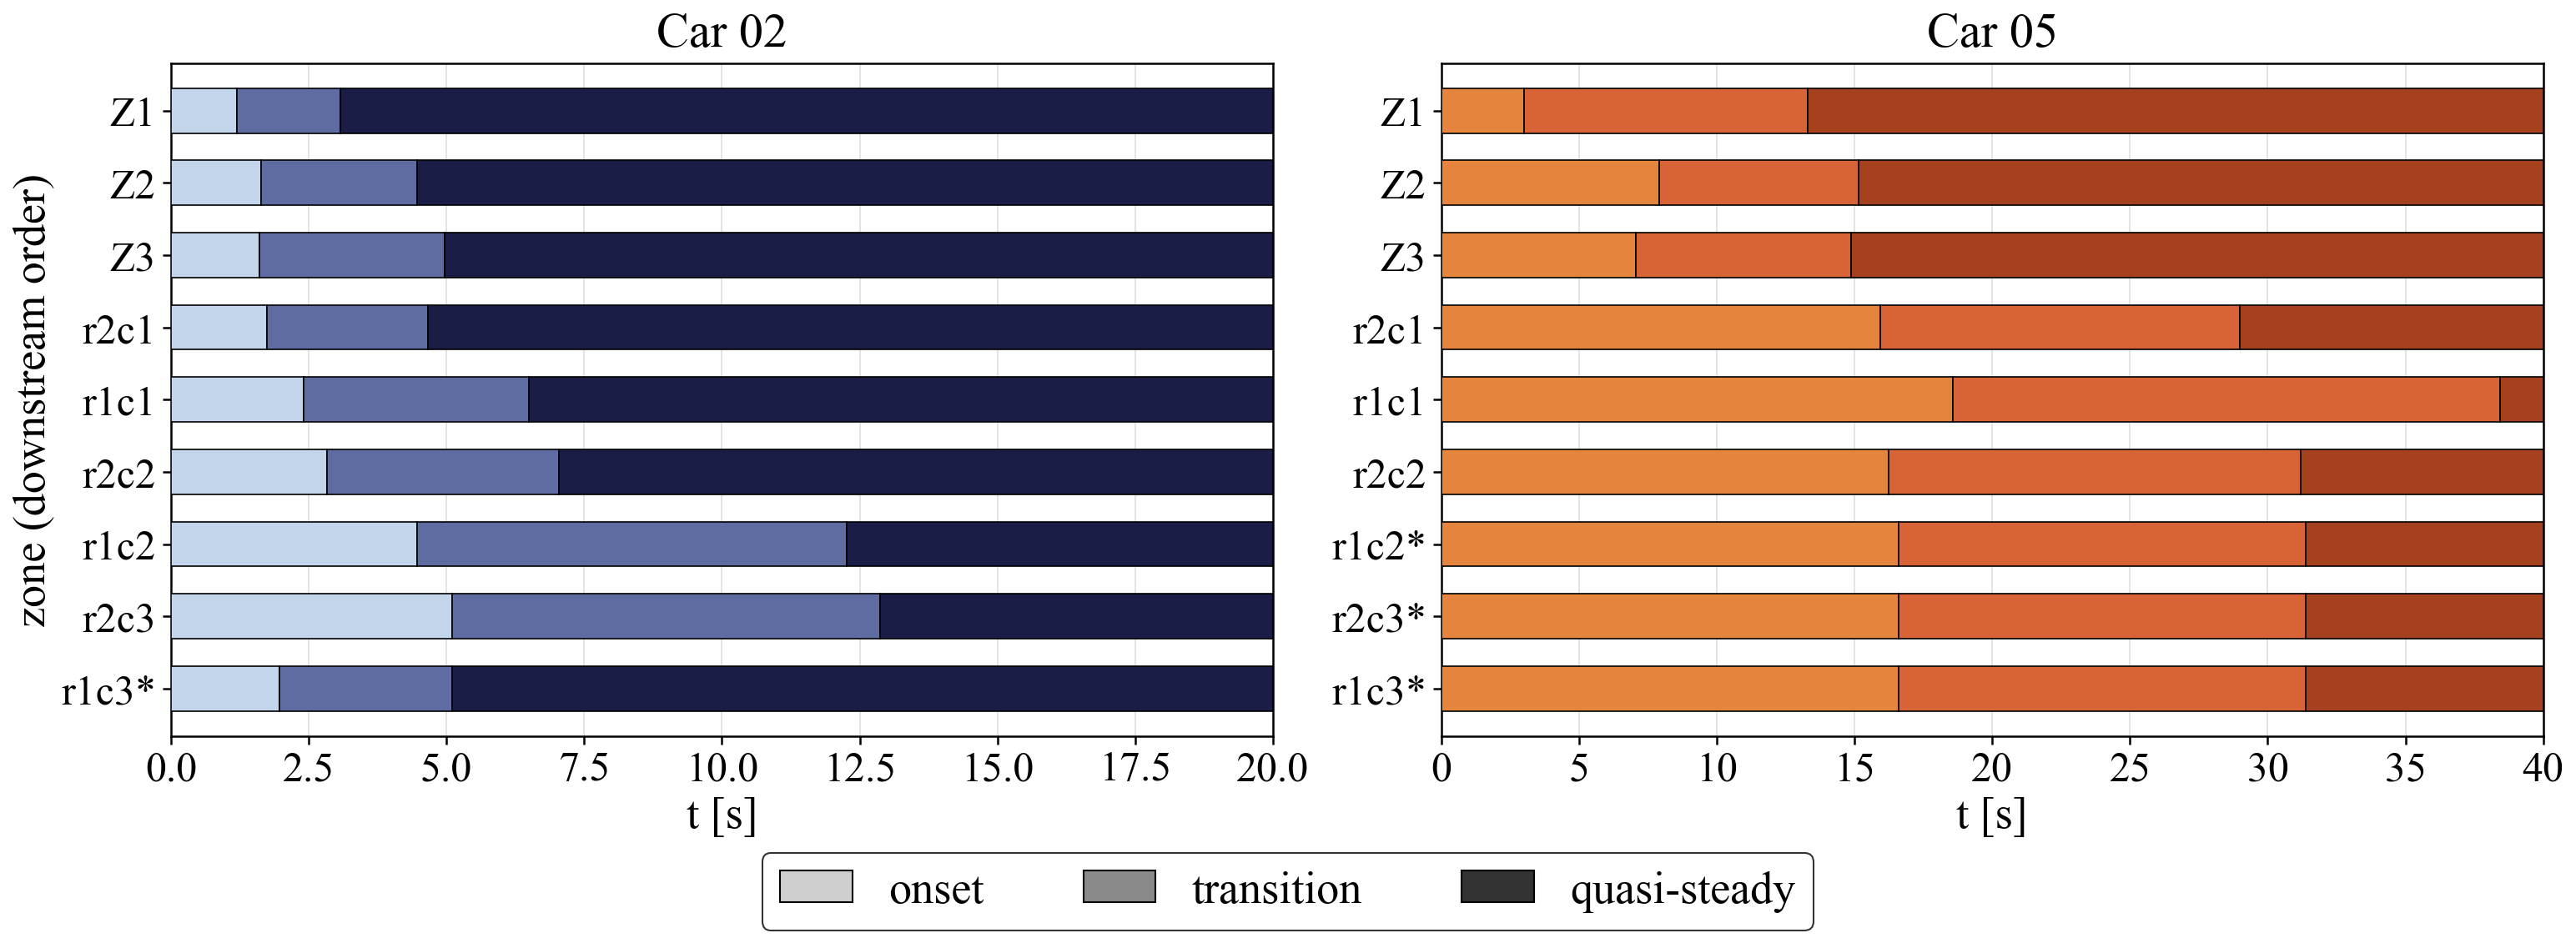
\includegraphics[width=0.9\textwidth]{Ilustraciones/flow_stages_gantt.png}
    \caption{Flow stages by zone for the fiber-free control of each formulation (Carbopol 0.2\%, left; Carbopol 0.5\%, right). Each horizontal bar is a zone, ordered from top to bottom along the downstream filling sequence, and is segmented into the onset, transition and quasi-steady stages.}
    \label{fig:flow_stages}
\end{figure}

% ------------------------------------------------------------
\subsection{Integration of the accumulated strain}
\label{sec:framework_strain}
% ------------------------------------------------------------

\textcolor{blue}{Redaccion revisada}

The independent variable of the saturation law is defined in Equation~\eqref{eq:accumulated_strain} as an integral along the path of a material element, whereas the PIV delivers an Eulerian field. Converting one into the other requires a trajectory, and the trajectory adopted here is that of the material occupying each cell of the partition, obtained by integrating the measured velocity field backward from the cell to the entry of the beam. The local shear rate $\dot{\gamma} = \sqrt{2\,\bm{D}\!:\!\bm{D}}$ is evaluated from the spatial derivatives of the same field along that path, and its integral over the time the material takes to traverse it gives the strain delivered to the population that arrests in the cell. The result is one value of $\Gamma$ per cell and per run, which is the resolution at which the law is traced.

\textcolor{red}{LLAMAR A LA FIGURA EN EL TEXTO}

\begin{figure}[htbp]
    \centering
    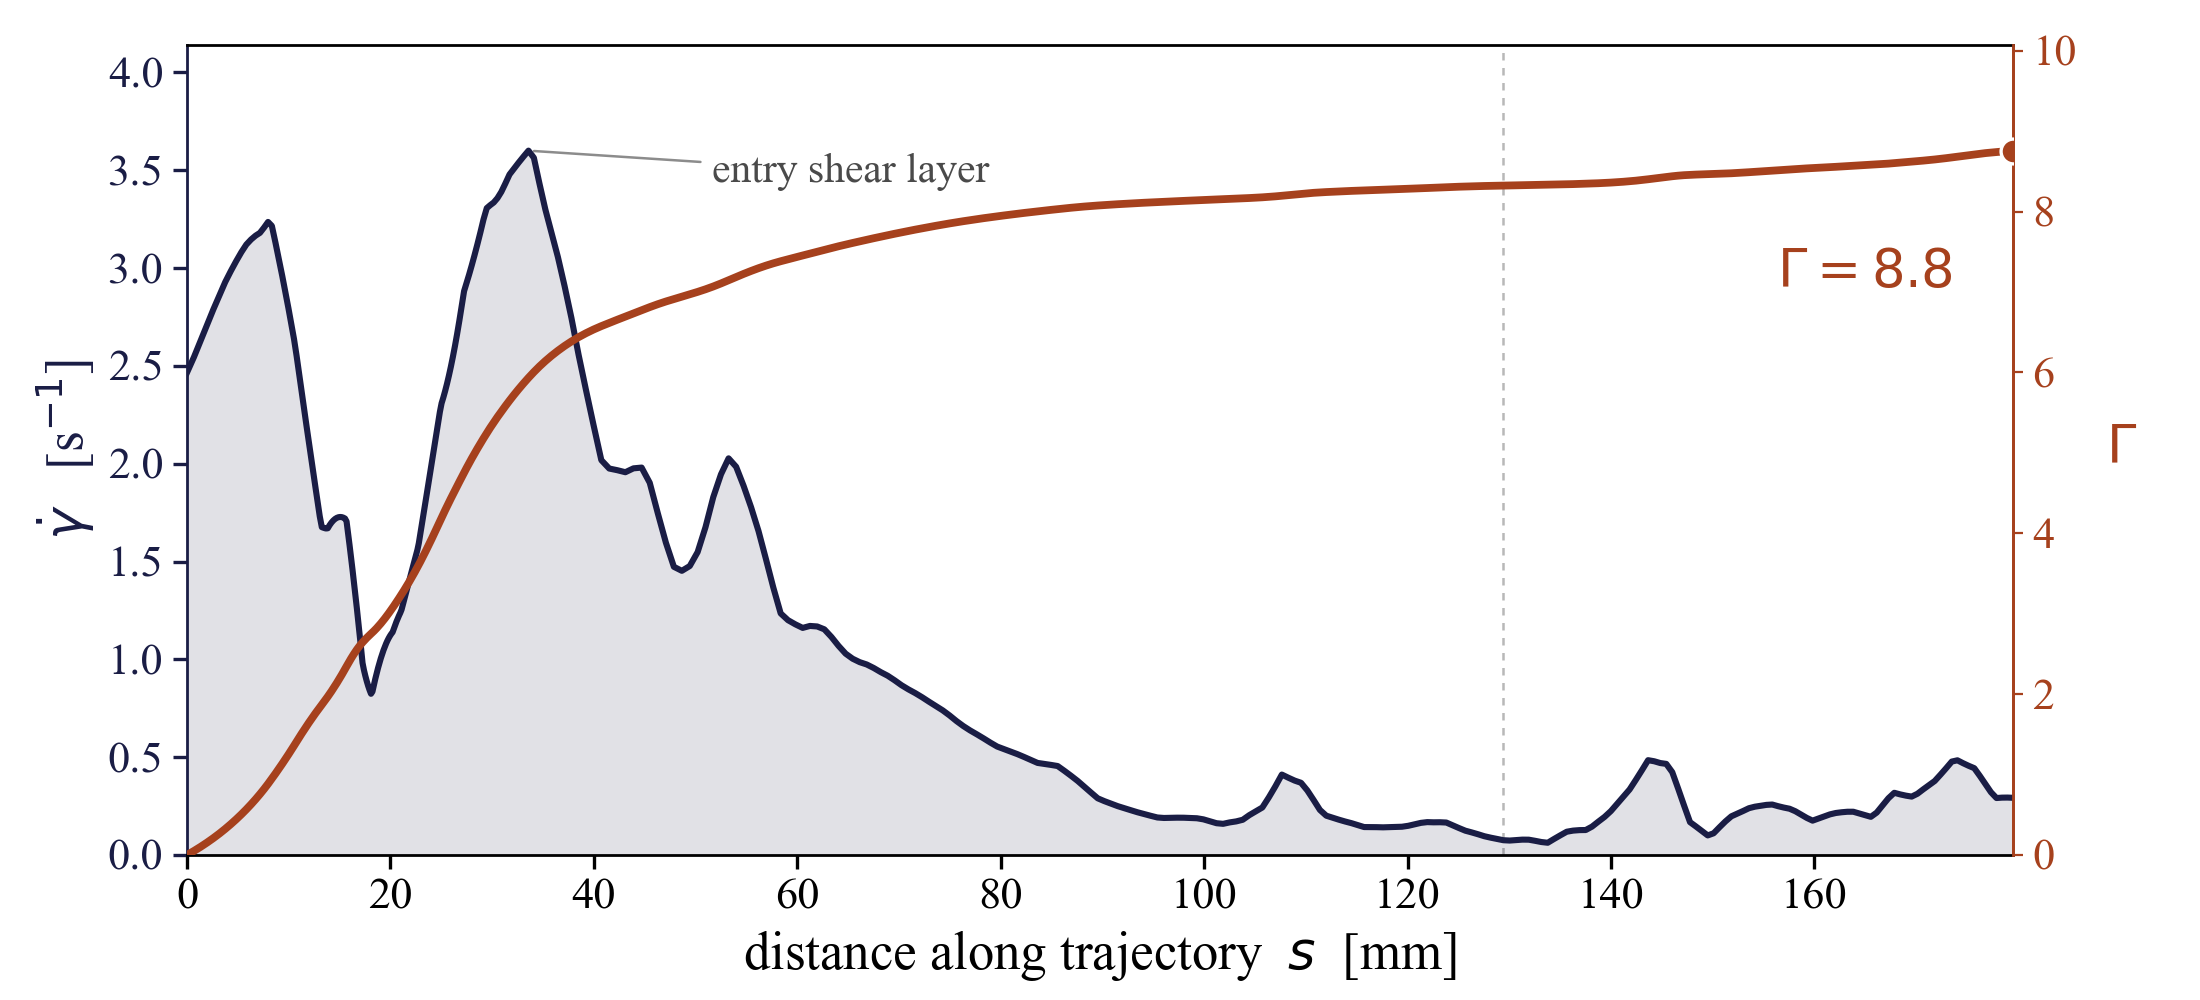
\includegraphics[width=0.9\textwidth]{Ilustraciones/PAPER_gamma_profile.png}
    \caption{Recovery of the accumulated strain along the path of the material arriving at cell r2c2, Carbopol 0.2\%. The local shear rate (left axis, grey) is evaluated from the spatial derivatives of the measured velocity field along the trajectory, and its integral along that path gives the accumulated strain (right axis). The deformation is delivered almost entirely within the entry shear layer, over the first third of the traverse, after which the material advances as a near-plug and the accumulated strain grows slowly toward its final value. This uneven delivery is what the yield stress produces and is the reason orientation is reported against $\Gamma$ rather than against position in the mold.}
    \label{fig:strain_integration}
\end{figure}

\textcolor{red}{QUITAR LINEAS PUNTEADAS DE LA FIGURA, ASI COMO MEJORAR ESTETICA}

The strain is measured on every run and not only on the fiber-free ones, because a suspension carrying more fibers advances more slowly than one carrying fewer, so the strain against which an orientation is read must be the strain that same suspension delivered. Reading orientation against position in the mold instead would conflate two distinct effects, the direct action of the fiber content on the alignment and the indirect action associated with the different amount of deformation the flow accumulated before reaching that position. This is the reason the results of Section~[REF] report orientation against $\Gamma$ rather than against the cell in which it was measured.

The origin from which $\Gamma$ is counted is the entry of the material into the beam, and not the inlet of the mold. The material does not flow smoothly from the outlet into the beam but falls and lands, and the impact against the accumulating deposit disorders the population, so the deformation delivered upstream does not carry forward into the state the fibers hold on arrival. The evidence supporting this reset is presented in Section~[REF], and it is what licenses the two parameter form of Equation~\eqref{eq:saturation}, in which the population is taken to enter with $\eta_{1,0}\approx 0$. That value is an assumption of simplicity and identifiability rather than a measured quantity: the tracking is planar while the angular state at the landing is three dimensional, so the entry order cannot be observed, and with the number of arrest points available per dosage it could not be identified alongside the ceiling and the strain scale in any case.

Placing the origin downstream of the bend serves a second purpose, independent of the reset. The accumulated strain of Equation~\eqref{eq:accumulated_strain} sums the magnitude of the deformation and is insensitive to its direction, so a flow that turns sharply continues to increase $\Gamma$ while the principal stretching direction rotates away from the direction in which the fibers have already been aligned. The monotone ordering assumed in Section~\ref{sec:governing} fails under those conditions, and the ninety degree bend of the present geometry is exactly such a turn. Tracing the law within the beam, downstream of the bend, keeps the analysis inside the domain of validity of the law it tests.

% ------------------------------------------------------------
\subsection{Provenance of the arrested fibers}
\label{sec:framework_provenance}
% ------------------------------------------------------------

\textcolor{red}{REVISAR LA REDACCIION DE ESTA SECCION}

Relating a final orientation to the deformation that produced it requires the path each arrested fiber followed, and the tracking does not supply those paths directly. At the loadings of the campaign the fraction of fibers followed continuously from entry to arrest is small, so each fiber is recovered as a series of short trajectory fragments rather than as a single unbroken track. The path is reconstructed by stitching those fragments forward in time, joining a fragment that ends to one that begins shortly afterwards whenever the two are consistent over the interval between them in three respects: in the position reached by advecting the fiber forward from its measured velocity, in the orientation predicted from its measured angular velocity, and in the detected length, which fixes the fiber size and rejects a join between objects of different apparent extent. The procedure is repeated until a chain spans the path from the vertical arm, through the elbow and the outlet, to the beam.

The tolerances are set conservatively everywhere except across the transition from the L-shape into the beam, where detection is interrupted and the gap between fragments is wider, and the policy throughout is that a doubtful join is refused rather than forced. The asymmetry is deliberate: a missing link ends a path early and shortens the reconstructed route, whereas a wrong one fabricates a trajectory no fiber followed and attributes to a population a deformation history it never received. The reconstructed paths are consequently shorter than the true ones and biased toward the fibers easiest to follow, which is a loss of completeness rather than of validity.

The provenance established in this way is checked against two independent attributions of the origin of each fiber, computed on the same population and compared. The first is the modal zone in which the fragments of a given chain were observed, which rests on the detections alone. The second is the zone reached by integrating the final position of the fiber backward along the measured PIV field, which rests on the carrier flow alone and uses no tracking information. The two attributions agree on the same population, so the routes are not an artifact of the stitching criteria.

Fig.~\ref{fig:fiber_routes} shows the routes recovered in this way, one row per destination cell. The L-shape is a common trunk, since by the geometry of the mold no fiber reaches the beam without traversing it in the order Z1, Z2, Z3, and the routes separate only afterwards, by destination. The contrast between the two formulations is what bounds the analysis that follows: Carbopol 0.2\% populates five of the six beam cells and reaches the far end, whereas Carbopol 0.5\% populates only three, clustered near the entry, and never reaches the third column, because the stiffer gel arrests while the beam is still half empty. The arrest points of the stiffer formulation are therefore confined to the low-strain region of the saturation curve, where they carry no information about its shape, which is one of the two reasons the fit of Section~\ref{sec:results_fit} is restricted to the softer formulation.

\begin{figure}[htb]
    \centering
    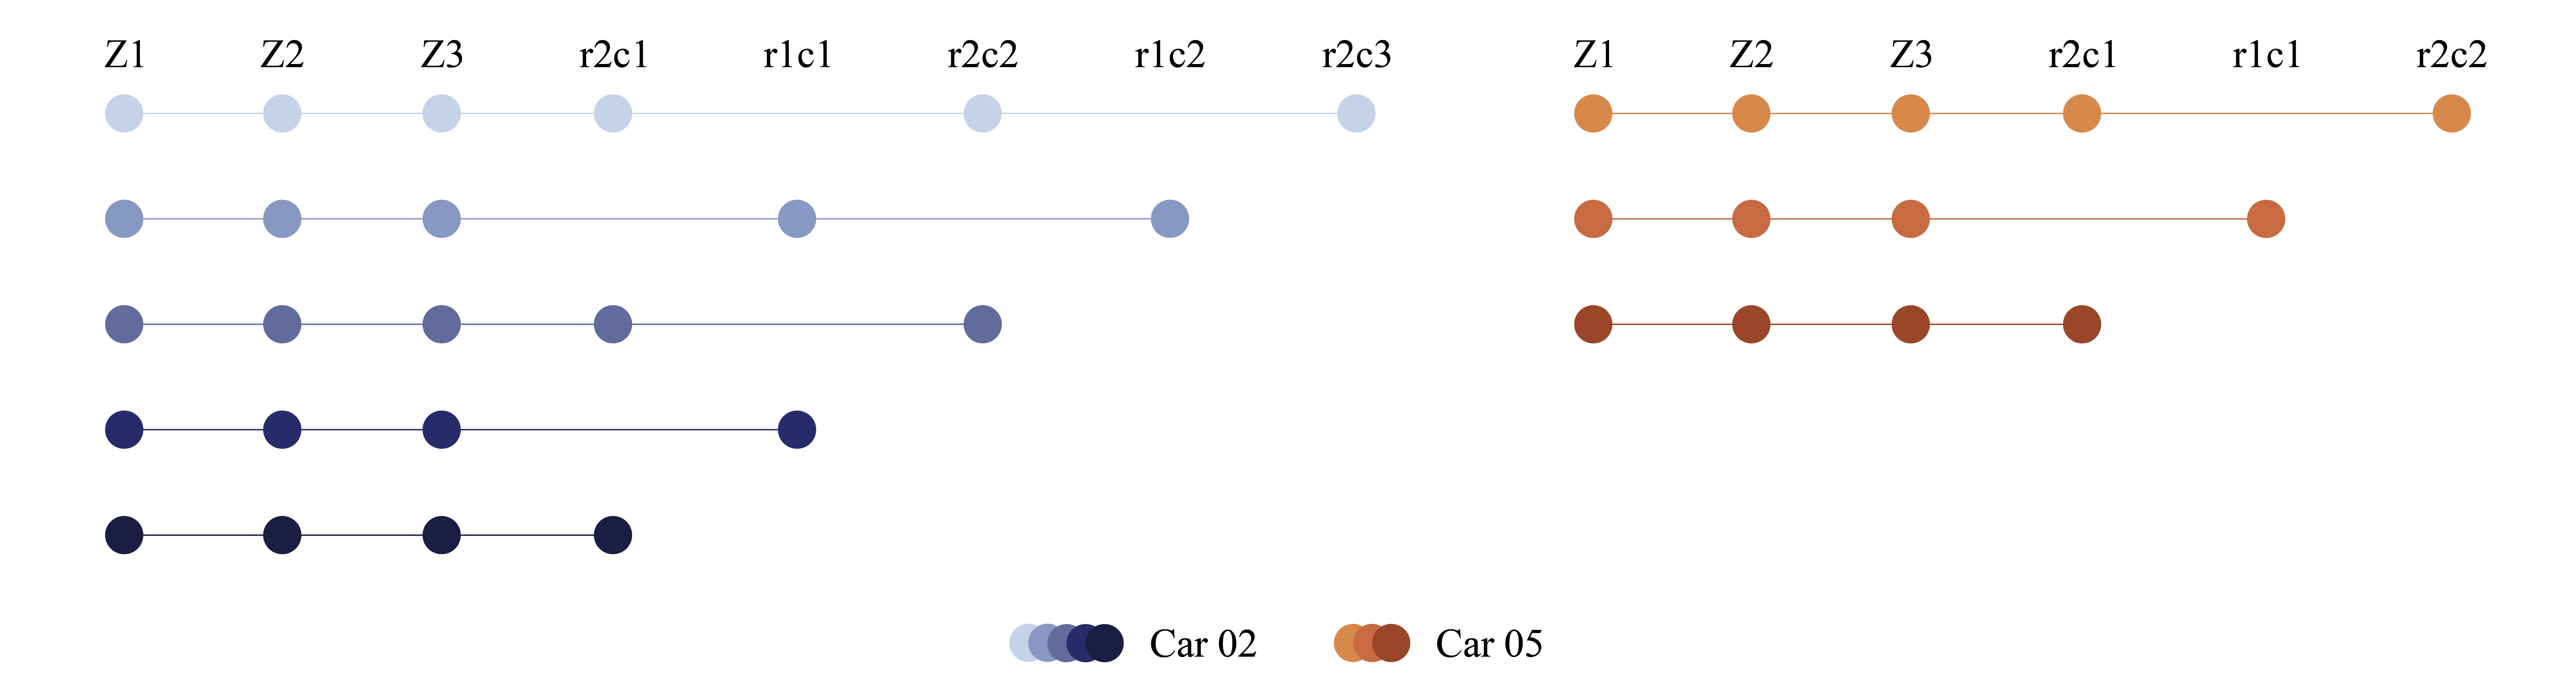
\includegraphics[width=0.9\textwidth]{Ilustraciones/RutasFibras.png}
    \caption{Routes followed by the fibers reaching each cell of the beam, reconstructed by stitching the trajectory fragments recovered by the tracking. Each row is one destination cell, and the marked zones are those its fibers traversed on the way. The three dosages are pooled. Left: Carbopol 0.2\%. Right: Carbopol 0.5\%. The stiffer formulation never reaches the third column of the beam, since it arrests while the beam is still half empty, so its arrest points sample only the low-strain region of the saturation curve.}
    \label{fig:fiber_routes}
\end{figure}

% ------------------------------------------------------------
\subsection{Uncertainty budget}
\label{sec:framework_uncertainty}
% ------------------------------------------------------------

Three sources of uncertainty bound the results reported in Section~\ref{sec:results}, and they are stated together so that the confidence attaching to each comparison is explicit. The first is the uncertainty of the velocity field, which is dominated by the sub-pixel displacement error and is therefore largest in relative terms where the mean velocity is lowest. Table~\ref{tab:piv_error} reports the total relative error for each camera and formulation, ranging from $10.0\%$ in the view covering the fastest region to $36.2\%$ in the slowest. That range does not propagate uniformly onto the accumulated strain. Because $\Gamma$ is an integral of the shear rate along the traverse, and the deformation is delivered almost entirely within the entry shear layer as Fig.~\ref{fig:strain_integration} shows, the cells carrying the largest relative error are those in which the material moves slowest and which therefore contribute least to the accumulated total. \textcolor{red}{[INSERTAR AQUÍ: la fracción de $\Gamma$ aportada por el tramo de mayor velocidad y su error asociado, del tipo "the first third of the traverse delivers approximately X\% of the accumulated strain and is measured at a relative error of Y\%, so the error on $\Gamma$ is bounded by Z\%". Es un solo número calculable desde la Fig. 4 y la Tabla IV.]}

\begin{table}[htb]
\centering
\caption{Total relative error of the PIV velocity field, by camera and Carbopol formulation. Percentage errors are referred to the mean flow speed $\bar{u}$ of each view. The sub-pixel displacement error dominates in all cases, so the relative uncertainty is highest where the mean speed is lowest.}
\label{tab:piv_error}
\begin{tabular}{
    c
    l
    S[table-format=2.1]
    S[table-format=2.1]
}
\toprule
\textbf{Camera} & \textbf{Car} &
  \multicolumn{1}{c}{\makecell{$\bar{u}$ \\ (mm\,s$^{-1}$)}} &
  \multicolumn{1}{c}{\makecell{$\delta u_{total}$ \\ (\%)}} \\
\midrule
\multirow{2}{*}{1} & 0.2\% & 27.7 & 10.6 \\
                   & 0.5\% &  6.1 & 14.8 \\
\midrule
\multirow{2}{*}{2} & 0.2\% & 12.6 & 21.8 \\
                   & 0.5\% &  2.4 & 13.3 \\
\midrule
\multirow{2}{*}{3} & 0.2\% &  9.4 & 36.2 \\
                   & 0.5\% &  1.7 & 16.1 \\
\midrule
\multirow{2}{*}{4} & 0.2\% & 39.5 & 10.0 \\
                   & 0.5\% & 15.0 & 11.3 \\
\bottomrule
\end{tabular}
\end{table}

The second concerns the detection of the fibers, which is orientation dependent for the reason set out in Section~\ref{sec:framework_ptv}. What the analysis requires is not that the detection rate reach unity, which no illumination can guarantee for a specular reflector, but that whatever fraction is lost should not vary systematically with the dosage, since a rate falling with concentration would produce an apparent change in the orientation statistics with no change in the fibers themselves. Table~\ref{tab:tracking_efficiency} shows that it does fall, from approximately $30$ to $42\%$ at the lowest loading to below $12\%$ at the highest, so the number of fibers recovered is itself a function of the dosage and a difference in sample size could masquerade as a difference in the population. Every trend with fiber content reported in Section~\ref{sec:results} is therefore evaluated on subsamples drawn to a common size across dosages, and a trend is retained only if it survives that control.

\begin{table}[htb]
\centering
\caption{Tracking efficiency by nominal fiber dosage and Carbopol formulation, computed as the ratio of detected to expected fibers within the field of view during the quasi-steady window. It bounds the effective sample size available for the analysis of each run.}
\label{tab:tracking_efficiency}
\begin{tabular}{
    l
    S[table-format=4.0]
    S[table-format=3.1]
    S[table-format=2.1]
}
\toprule
\textbf{Car} &
  \multicolumn{1}{c}{\makecell{Nominal \\ $N$}} &
  \multicolumn{1}{c}{\makecell{Detected \\ fibers}} &
  \multicolumn{1}{c}{\makecell{Efficiency \\ (\%)}} \\
\midrule
\multirow{3}{*}{0.2\%} &  750 & 162.5 & 29.7 \\
                       & 1500 & 191.7 & 17.5 \\
                       & 3000 & 168.7 &  7.7 \\
\midrule
\multirow{3}{*}{0.5\%} &  750 & 227.6 & 41.6 \\
                       & 1500 & 264.1 & 24.1 \\
                       & 3000 & 244.7 & 11.2 \\
\bottomrule
\end{tabular}
\end{table}

The third is the planar projection of an orientation that is in general three dimensional. Each fiber is recovered from a single camera, which locates it within the image plane but not along the optical axis, and measures the projection onto that plane of its orientation. A rod inclined out of the plane projects toward the projection axis, so out-of-plane fibers appear more aligned with the imaging plane than they are and the measured order parameter overestimates the alignment of the three dimensional population. The bias is systematic and signed, and two circumstances bound it. The flow is confined between two walls separated by a distance small compared with the length of the mold, so the out-of-plane velocity component is small and the fibers have little occasion to acquire a large inclination. And the bias, acting in the same direction at every dosage, displaces the curves of the saturation law together rather than manufacturing a separation between them: the reservation therefore attaches to the absolute value of the fitted ceiling and not to its ordering across fiber contents, which is the comparison the measurements are asked to support.

% ------------------------------------------------------------
\subsection{Statistical protocol}
\label{sec:framework_stats}
% ------------------------------------------------------------

Two questions recur throughout Section~\ref{sec:results}: whether the rheology of the carrier affects a given quantity, and whether the fiber content does. Both are answered under a common protocol, so that the effect sizes reported across zones, stages, formulations and variables are directly comparable. Table~\ref{tab:quantities} collects the quantities on which that protocol operates. The carrier is described in an Eulerian frame through its speed $|\bm{u}|$ and the magnitude of the out-of-plane vorticity $|\zeta|$, the symbol $\zeta$ being reserved for the fluid so as not to collide with the fiber angular velocity $\omega$, since both are rotation rates. The fibers are described in a Lagrangian frame through their speed $|\bm{v}|$, their angular velocity $\omega$, and three descriptors of the state of the population within a region: the order parameter $\eta_1$ of Equation~\eqref{eq:eta_1}, recovered in the imaging plane as $|\langle e^{i2\theta}\rangle|$ over the fibers of the region, which is identical to the eigenvalue form under the planar reduction; the angular deviation $\delta$ of each fiber from the director of its region; and the dispersion index $\Lambda$, which compares the radius of gyration of the fiber centroids with that of a uniform arrangement over the same cell, so that $\Lambda = 1$ denotes a uniform arrangement, $\Lambda < 1$ clustering, and $\Lambda > 1$ an arrangement displaced toward the boundaries of the cell.

\begin{table}[htb]
\centering
\caption{Quantities used throughout the analysis. Carrier quantities are measured by PIV, fiber quantities by PTV.}
\label{tab:quantities}
\begin{tabular}{c l c l}
\toprule
\textbf{Symbol} & \textbf{Quantity} & \textbf{Phase} & \textbf{Range and meaning} \\
\midrule
$|\bm{u}|$ & Carrier speed          & PIV & $\geq 0$ \\
$|\zeta|$  & Carrier vorticity      & PIV & $\geq 0$; local rotation rate of the fluid \\
$|\bm{v}|$ & Fiber speed            & PTV & $\geq 0$ \\
$\omega$   & Fiber angular velocity & PTV & Rotation rate of the fiber axis \\
$\hat{\eta}_1$ & Orientation order  & PTV & $0$ isotropic $\rightarrow$ $1$ fully aligned \\
$\delta$   & Angular deviation      & PTV & $[0^\circ,90^\circ]$; misalignment from the director \\
$\Lambda$  & Spatial dispersion     & PTV & $<1$ clustered; $1$ uniform; $>1$ over-dispersed \\
\bottomrule
\end{tabular}
\end{table}

The order parameter and the angular deviation describe the same state from opposite ends, and the distinction governs which of the two is used where. The order parameter is a property of the population, computed as a single number from all the fibers of a cell, so it is the natural response when the question concerns the degree of alignment a cell has reached, and it is the quantity the saturation law predicts. The angular deviation is a property of each fiber, so it supplies one observation per fiber rather than one per cell, and it is the natural response when a test must be resolved within a single cell with enough degrees of freedom to be meaningful. A rise in $\delta$ and a fall in $\eta_1$ describe the same physical event, namely a loss of order.

The filling is transient, so the effect of a factor cannot be read from a simple mean: the same zone passes through very different flow conditions as the mold fills. Every test is therefore an analysis of covariance with time entered as a continuous covariate, so that the shared temporal trend is removed before the factor of interest is evaluated. The strength of the factor is reported as the partial eta squared,

\begin{equation}
    \eta^2_p = \frac{SS_{factor}}{SS_{factor} + SS_{error}},
    \label{eq:partial_eta_squared}
\end{equation}

the share of variance the factor explains once the variance attributable to the other terms has been removed. Unlike the ordinary eta squared, whose denominator is the total variance, the partial form does not shrink as further factors are added, which is what makes effect sizes from different models comparable; it is written $\eta^2$ throughout.

Effect size rather than significance is the primary criterion, and the two questions are settled by separate numbers: the $p$ value of the term at $\alpha = 0.05$ for whether an effect is distinguishable from zero, and the magnitude of $\eta^2$ for how large it is. A relevance threshold of $\eta^2 \geq 0.02$ is adopted throughout, placed just above the conventional small-effect boundary so that it acts as a noise floor, with values below it reported but not interpreted however small their $p$ value; the conventional bands at $\eta^2 \geq 0.10$ and $\eta^2 \geq 0.30$ mark moderate and strong effects in the tables that follow [CITAR]. The threshold guards against a specific failure of this dataset. Most tests are run on the populated zones, where the observations number in the hundreds or thousands, so the standard error is minute and an effect explaining less than one percent of the variance is still flagged as significant. The threshold is what keeps such an effect from being read as a result.

The opposite failure occurs where the data are sparse, and is guarded against separately. The distal cells of the beam, and every cell of the stiffer formulation beyond the second column, hold too few fibers to support a test, and a fluctuation computed over a few dozen observations can return a large effect size on a $p$ value that establishes nothing. Such cells are not reported: the tables are restricted, within each formulation, to the zones the flow actually reaches, a zone being retained only where the carrier establishes a resolved velocity field and a countable population of fibers is tracked.

A further control is applied wherever the fiber content is the factor, and it is not optional, because the measurement and the hypothesis act on the same quantity in the same direction. The detection efficiency falls with the loading (Table~\ref{tab:tracking_efficiency}), so a cell of a richer suspension is described by a smaller sample of fibers than the same cell of a leaner one, and the order parameter carries a finite-sample bias that falls as the sample grows, since $\mathbb{E}[\eta_1^2] \simeq 1/n$ for $n$ fibers drawn from an isotropic distribution. A cell holding fewer fibers therefore returns a higher spurious order. The bias acts against the hypothesis at high dosage and would mask the effect rather than manufacture it, but it also varies from cell to cell with the count, so an uncorrected comparison across dosages would confound the physical trend with the sampling. Two measures address this. The order parameter is reported throughout in its debiased form,

\begin{equation}
    \hat{\eta}_1^{\,2} = \frac{n\,\eta_1^2 - 1}{n - 1},
    \label{eq:eta_debiased}
\end{equation}

which is unbiased to leading order for an isotropic population and reduces to $\eta_1$ as the count grows. And wherever a trend with the dosage is claimed, the tracked fibers are bootstrap-resampled to an equal count across the three levels, and the trend is retained only if it survives in the majority of resamples; a trend that does not survive is an artifact of unequal sampling and not a physical effect.

The distinction between a zonal and a pooled effect is used deliberately and requires a word, since the two answer different questions. Pooling averages the whole domain at once, and the domain spans conditions as different as a plug descending the arm and a nearly arrested cell of the beam; that spatial variation is far larger than the effect of the fibers, so it dominates the pooled figure and drives it toward zero. A pooled value therefore measures how small the fiber effect is relative to the spatial variation of the flow, which is a property of the geometry, whereas the zonal values measure the effect itself. Both are reported, and where they differ the interpretation rests on the zonal ones.

% ============================================================
\section{Results}
\label{sec:results}
% ============================================================

\textcolor{blue}{Redaccion revisada}

The results are reported in four movements. The first two establish that the two mechanisms the saturation law rests on are present in this flow: that the fibers perturb the carrier and rotate faster as their number grows, and that the alignment they retain once the material has arrested falls as the dosage rises. Both are consequences of the interaction term of Equation~\eqref{eq:advani_tucker}, and their presence is what licenses the reduction of Section~\ref{sec:governing} in a flow lying outside the conditions for which the model was derived. The third movement fixes the origin from which the accumulated strain is counted. The fourth fits the law and tests it predictively.

% ------------------------------------------------------------
\subsection{Perturbation of the carrier and rotation of the fibers}
\label{sec:results_kinematics}
% ------------------------------------------------------------

\textcolor{blue}{Redaccion revisada}

The effect of the fiber content on each Eulerian and Lagrangian quantity was evaluated zone by zone and stage by stage under the protocol of Section~\ref{sec:framework_stats}. Table~\ref{tab:ancova_combined} report, for each variable and stage, the largest effect found anywhere in the domain together with the zone in which it occurs, and the effect in every zone is given in the supplementary material.

\begin{table}[htb]
\centering
\caption{Effect of fiber content on the Eulerian and Lagrangian variables, by flow stage and matrix. Peak columns report the largest $\eta^{2}$ found across all spatial zones, with the zone of maximum effect in parentheses; pooled columns report $\eta^{2}$ computed over the whole domain at once. The two answer different questions: the pooled value is small because the spatial variation of the flow is far larger than the effect of the fibers, so it measures the effect relative to the geometry rather than the effect itself. Carrier quantities are measured by PIV, fiber quantities by PTV. $^{*}$~$\eta^{2} \geq 0.02$;\; $^{**}$~$\eta^{2} \geq 0.10$;\; $^{***}$~$\eta^{2} \geq 0.30$.}
\label{tab:ancova_combined}
\small
\setlength{\tabcolsep}{4pt}
\begin{tabular}{l l l l l c c c}
\toprule
 & & \multicolumn{3}{c}{\textbf{Peak} $\boldsymbol{\eta^{2}}$ \textbf{(zone)}}
   & \multicolumn{3}{c}{\textbf{Pooled} $\boldsymbol{\eta^{2}}$} \\
\cmidrule(lr){3-5}\cmidrule(lr){6-8}
\textbf{Variable} & \textbf{Car}
  & \textbf{Onset} & \textbf{Trans.} & \textbf{QS}
  & \textbf{Onset} & \textbf{Trans.} & \textbf{QS} \\
\midrule
\multicolumn{8}{l}{\textit{Translational}} \\
\addlinespace[1pt]
\multirow{2}{*}{$|\mathbf{u}|$ \; carrier}
  & 0.2\,\% & 0.165$^{**}$ (r1c1) & 0.102$^{**}$ (Z2)   & 0.049$^{*}$ (Z2)    & 0.002 & 0.004 & 0.005 \\
  & 0.5\,\% & 0.292$^{**}$ (Z2)   & 0.434$^{***}$ (Z2)  & 0.525$^{***}$ (r1c1) & 0.007 & 0.004 & 0.008 \\
\addlinespace[2pt]
\multirow{2}{*}{$|\mathbf{v}|$ \; fiber}
  & 0.2\,\% & 0.165$^{**}$ (r2c2) & 0.279$^{**}$ (Z1)   & 0.396$^{***}$ (r2c3) & 0.001 & 0.032$^{*}$ & 0.022$^{*}$ \\
  & 0.5\,\% & 0.161$^{**}$ (Z1)   & 0.091$^{*}$ (Z1)    & 0.368$^{***}$ (r2c1) & 0.006 & 0.005 & 0.007 \\
\midrule
\multicolumn{8}{l}{\textit{Rotational}} \\
\addlinespace[1pt]
\multirow{2}{*}{$|\zeta|$ \; carrier}
  & 0.2\,\% & 0.283$^{**}$ (Z1)   & 0.228$^{**}$ (Z1)   & 0.061$^{*}$ (r2c3)   & 0.000 & 0.000 & 0.001 \\
  & 0.5\,\% & 0.094$^{*}$ (Z3)    & 0.095$^{*}$ (Z3)    & 0.160$^{**}$ (r2c2)  & 0.001 & 0.001 & 0.003 \\
\addlinespace[2pt]
\multirow{2}{*}{$|\omega|$ \; fiber}
  & 0.2\,\% & 0.426$^{***}$ (Z1)  & 0.502$^{***}$ (Z1)  & 0.358$^{***}$ (r2c2) & 0.051$^{*}$ & 0.050$^{*}$ & 0.062$^{*}$ \\
  & 0.5\,\% & 0.333$^{***}$ (Z1)  & 0.327$^{***}$ (Z1)  & 0.430$^{***}$ (r2c1) & 0.039$^{*}$ & 0.050$^{*}$ & 0.110$^{**}$ \\
\midrule
\multicolumn{8}{l}{\textit{Orientation}} \\
\addlinespace[1pt]
\multirow{2}{*}{$\eta_{1}$ \; fiber}
  & 0.2\,\% & 0.284$^{**}$ (Z2)   & 0.161$^{**}$ (r2c1) & 0.713$^{***}$ (r2c1) & 0.017 & 0.000 & 0.045$^{*}$ \\
  & 0.5\,\% & 0.407$^{***}$ (Z1)  & 0.523$^{***}$ (r2c1) & 0.384$^{***}$ (Z2)  & 0.035$^{*}$ & 0.028$^{*}$ & 0.009 \\
\bottomrule
\end{tabular}
\end{table}

The carrier slows as the fiber content rises, in both formulations and at every stage, which is what the added hydrodynamic resistance of the fibers would produce. Where the effect concentrates it is large, reaching a partial eta squared of $0.525$ in the first cell of the beam in the stiffer matrix. The two formulations channel it differently, and the difference follows from their resistance to yielding: the softer gel yields readily across most of the domain, so its translational field is set by gravity and is comparatively insensitive to the loading, whereas the stiffer gel operates closer to its yield threshold over wider regions, so that adding fibers raises the effective consistency enough to shift whole regions between the yielded and the arrested state and thereby to alter the local advance velocity. The rheology does not determine whether the fibers perturb the flow, but which component of it they perturb.

The vorticity of the carrier behaves differently, and the contrast is the result on which the rest of this subsection turns. Where the speed responds most strongly, in the stiffer matrix, the vorticity responds least: the effect on the speed rises to $0.525$ while the effect on the vorticity never exceeds $0.160$ anywhere in that matrix, and pooled over the domain the vorticity effect does not exceed $0.003$ in either formulation. The rotational field of the carrier is therefore largely indifferent to how many fibers it contains, even where its translational field is not.

\textcolor{red}{LLAMAR A LA FIGURA EN EL TEXTO}

\begin{figure}[htb]
    \centering
    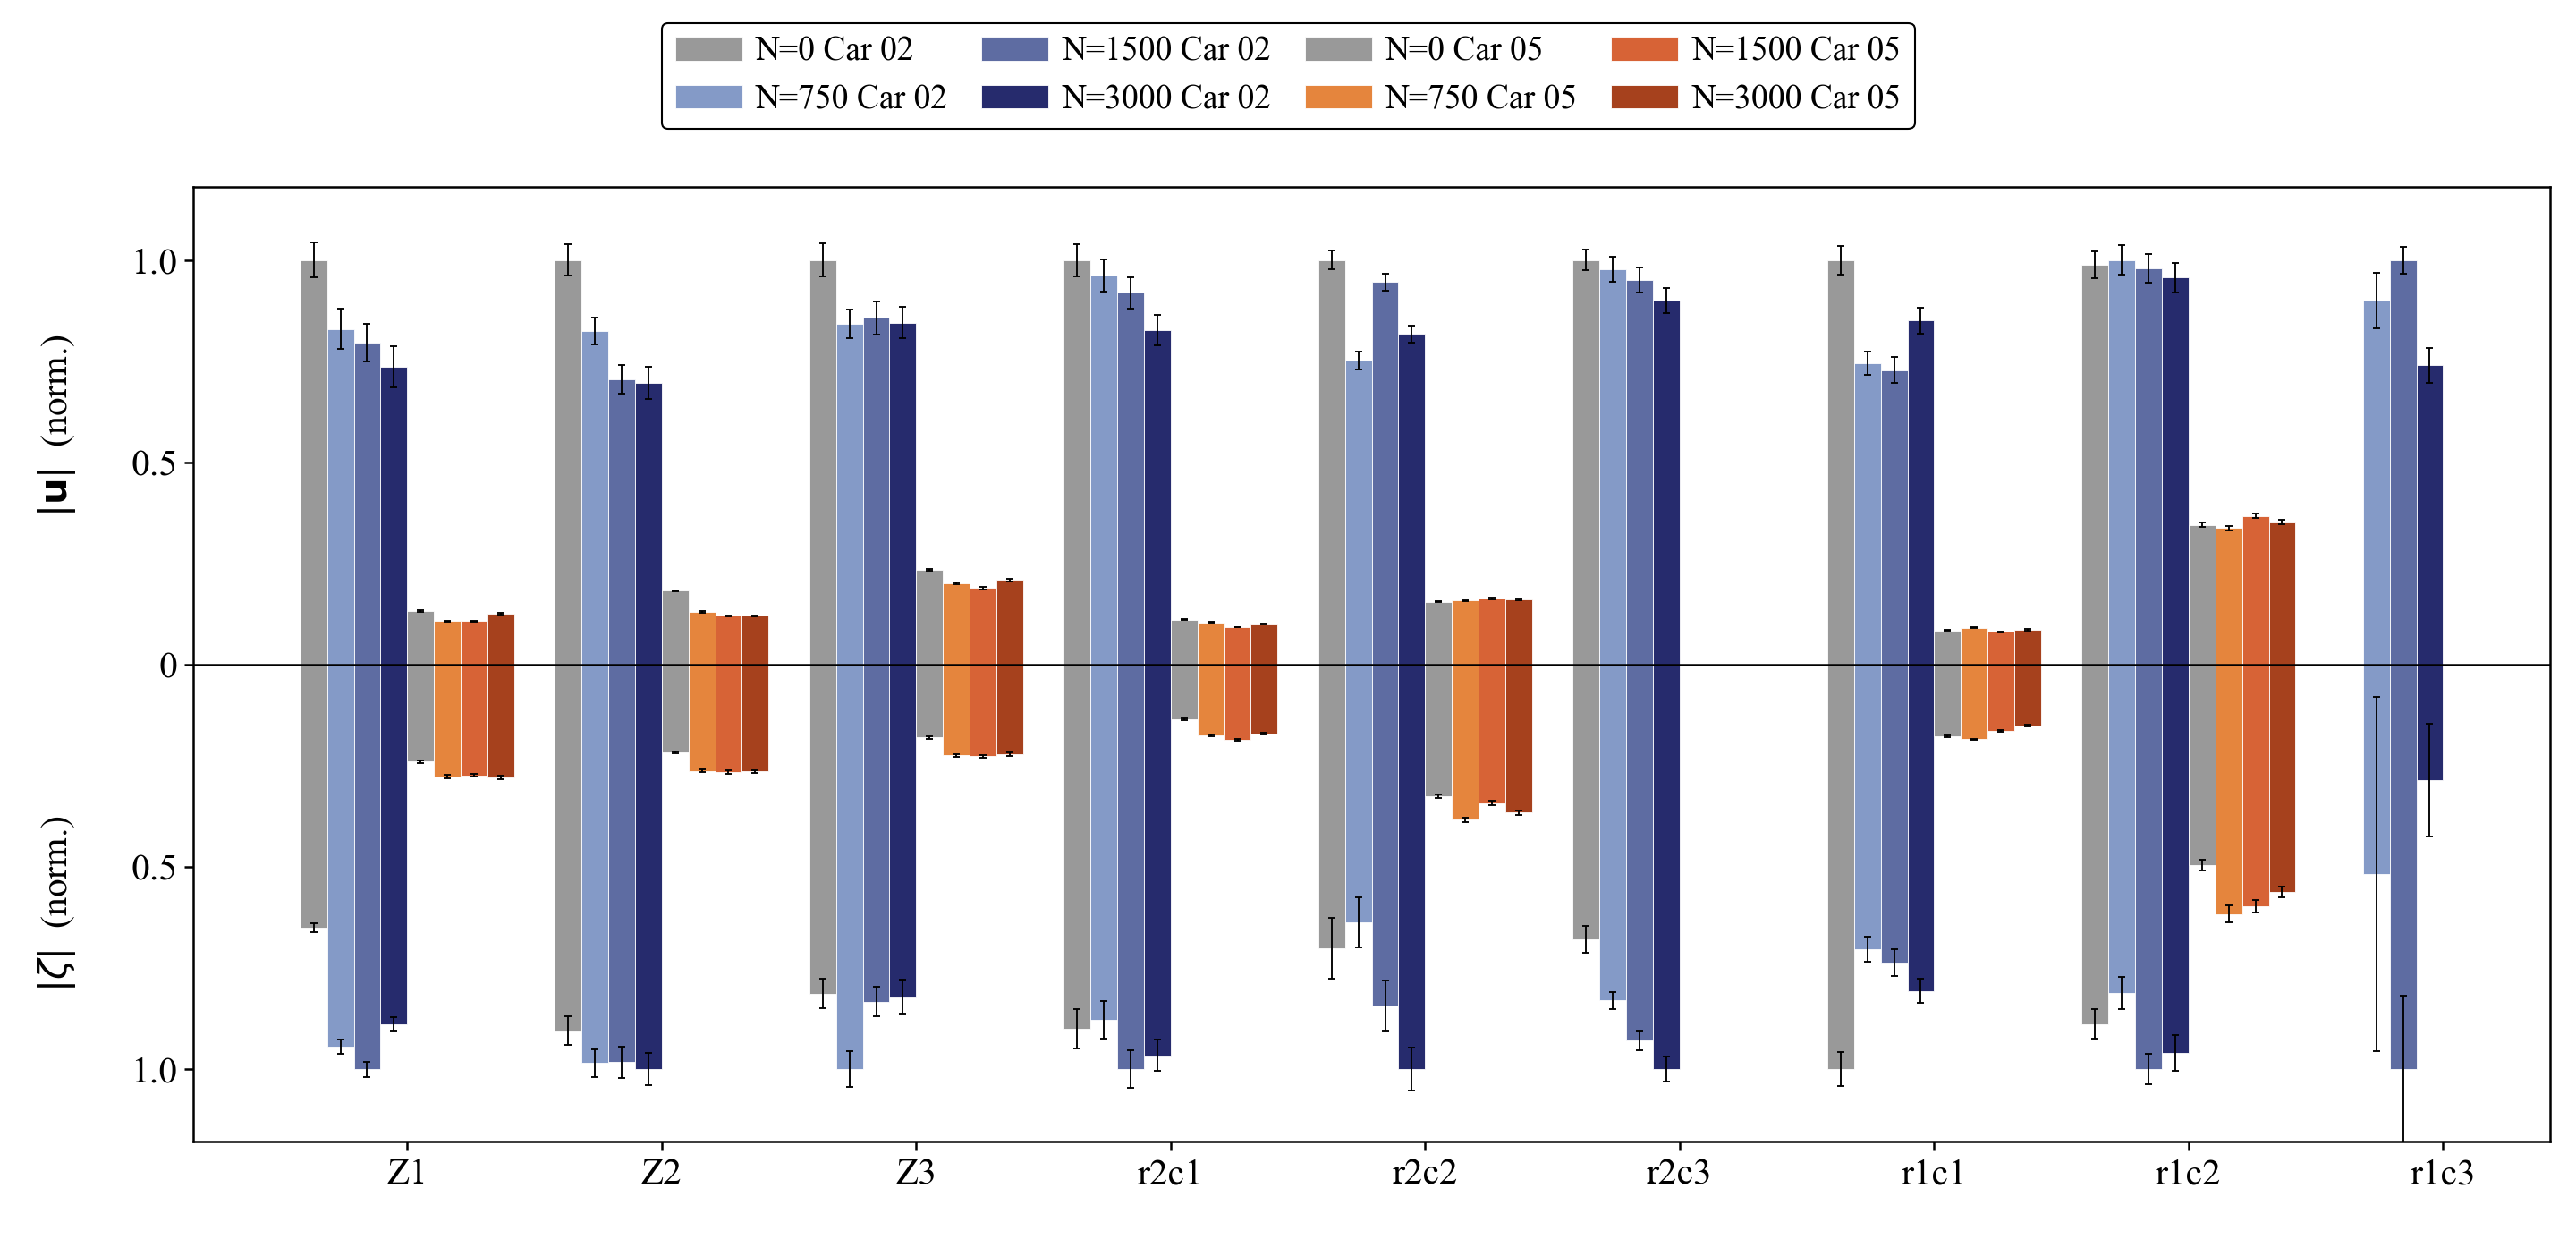
\includegraphics[width=1.0\textwidth]{Ilustraciones/PAPER_piv_mirror.png}
    \caption{Caption.}
    \label{fig:cambiar}   
\end{figure}

Against that background, the angular velocity of the fibers is the quantity most consistently modulated by the fiber content. It carries a relevant effect in nearly every zone and stage, reaching $0.502$ in the vertical arm of the softer matrix during the transition and $0.430$ in the first cell of the beam of the stiffer matrix once the flow has settled, and it is the only variable whose pooled effect survives the relevance threshold at every stage and in both formulations. The fiber content therefore raises the rotation of the fibers across the domain as a whole and not merely in particular regions.

This rotation is not inherited from the carrier. The pooled effect of the fiber content on the vorticity of the fluid does not exceed $0.003$, while the pooled effect on the angular velocity of the fibers reaches $0.110$, a difference of more than an order of magnitude between two rotation rates measured on the same flow. A fiber rotation supplied by the turning of the fluid would require the fluid to turn faster as fibers are added, which it does not. The additional rotation therefore originates outside the mean flow, and its magnitude grows with the fiber content, which is the behavior the interaction term of Equation~\eqref{eq:advani_tucker} represents. What the measurement provides here is direct kinematic evidence of that term, read from the motion of the fibers themselves rather than inferred from the orientation distribution they leave behind.

\textcolor{red}{LLAMAR A LA FIGURA EN EL TEXTO}

\begin{figure}[htb]
    \centering
    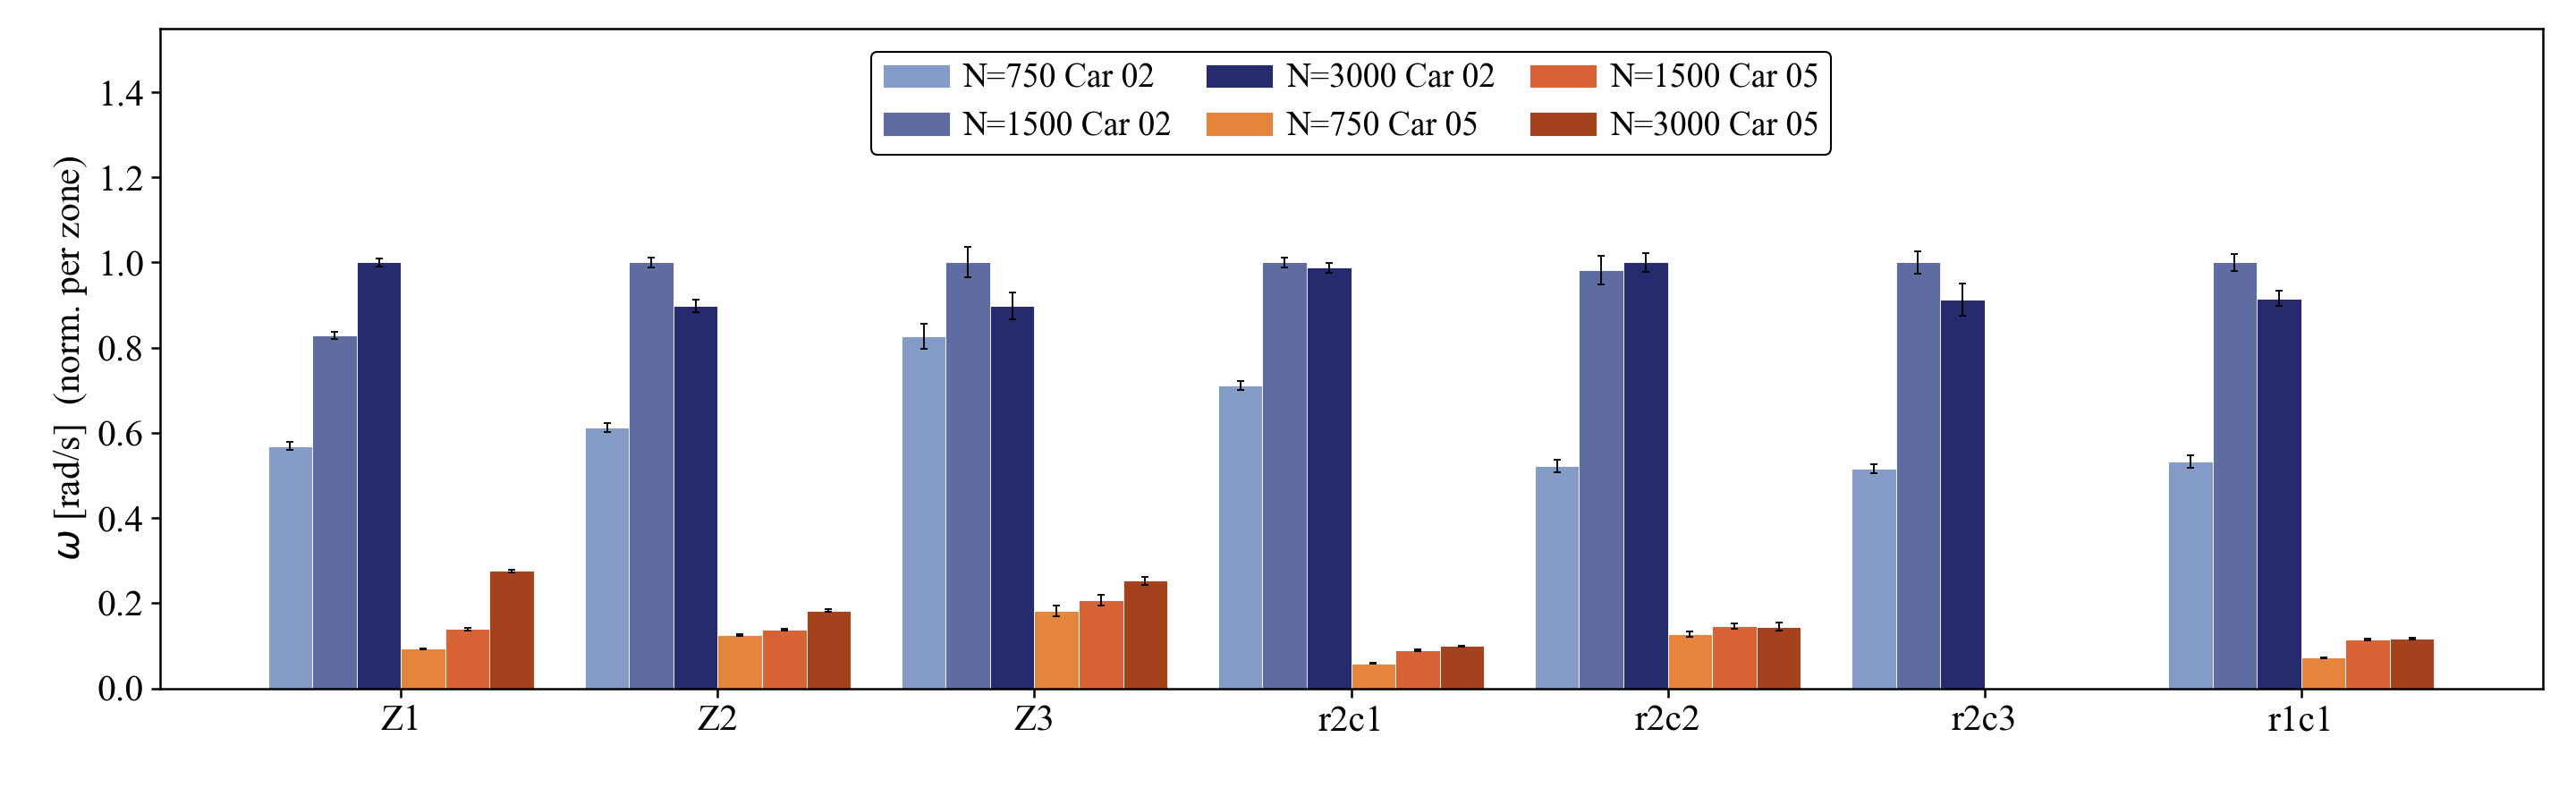
\includegraphics[width=1.0\textwidth]{Ilustraciones/ENT_ptv_omega.png}
    \caption{Caption.}
    \label{fig:cambiar}
\end{figure}

One feature of the Lagrangian data requires care before proceeding. The fiber speed rises with the fiber content, which is the opposite of the fall the PIV records in the fluid speed of the same runs, and taken at face value would have the fibers moving faster than the fluid that carries them. The discrepancy is instrumental. The PIV resolves the single plane lit by the laser sheet, whereas the PTV recovers fibers through the whole depth of the mold without resolving where in that depth each one lies, so the fibers are drawn in part from regions the velocity field never measures, including the faster core. The two speeds cannot be compared directly, and the fiber speed is used here only as a relative quantity across dosages within the tracking data. Whether the fibers lead or lag the carrier is a question a planar measurement cannot settle. The rotational decoupling reported above is of a different kind, since it compares the response of two rotation rates to a change in dosage rather than their absolute values, and is unaffected by the sampling mismatch.

% ------------------------------------------------------------
\subsection{The state the fibers settle into}
\label{sec:results_final_state}
% ------------------------------------------------------------

\textcolor{blue}{Redaccion revisada}

The quantities of the previous subsection are instantaneous, and an elevated rotation during filling does not by itself imply an altered orientation once the material has come to rest. This subsection establishes what survives arrest, and it does so only to the extent required by what follows: the hierarchy of the factors that govern the final state, and the direction in which the fiber content displaces it.

An analysis of covariance over the pooled domain, with the arrest zone, the rheological matrix and the fiber content as predictors of the angular deviation and of the spatial dispersion of the arrested population, gives an unambiguous hierarchy and the same one for both responses. The zone in which a fiber comes to rest dominates, exceeding every other factor by at least a factor of six and, for the orientation, by more than twenty. The matrix is second and is the only other factor to cross the relevance threshold, which it does for the dispersion alone. The fiber content, pooled over the dataset, is negligible for both.

\textcolor{red}{LLAMARA A LA TABLA EN EL TEXTO}

\begin{table}[htb]
\centering
\caption{Effect size $\eta^{2}$ of the principal determinants of the fiber final state, from the global Analysis of Covariance over the pooled domain. The relevance threshold of Section~\ref{sec:analysis_metrics} is $\eta^{2} = 0.02$.}
\label{tab:final_state_hierarchy}
\begin{tabular}{l S[table-format=1.4] S[table-format=1.4]}
\toprule
\textbf{Factor} & {\textbf{$\eta^{2}$ orientation ($\delta$)}} & {\textbf{$\eta^{2}$ dispersion ($\Lambda$)}} \\
\midrule
Final zone (geometry) & 0.0310 & 0.1880 \\
Rheological matrix    & 0.0014 & 0.0290 \\
Fiber content         & 0.0007 & 0.0001 \\
\bottomrule
\end{tabular}
\end{table}

The pooled figure understates the effect of the dosage, for the reason set out in Section~\ref{sec:framework_stats}: geometry is an order of magnitude stronger, and an influence confined to a few zones is averaged away once the domain is pooled. Repeating the analysis separately within each matrix, with the arrest zone retained as a covariate so that the fiber effect is measured net of the dominant geometric one, separates the two responses. The dispersion does not respond to the fiber content within either matrix. The orientation does: the effect grows by an order of magnitude over its pooled value, it is significant in both matrices, and the angular deviation rises with the fiber content at fixed rheology, which is to say that the fibers align less well as their number grows. The trend survives the resampling control of Section~\ref{sec:framework_uncertainty}, so it is not an artifact of the unequal detection statistics.

\textcolor{red}{LLAMAR A LA TABLA EN EL TEXTO}

\begin{table}[htb]
\centering
\caption{Net effect of fiber content on the final state, isolated from the geometric effect within each rheological matrix. The relevance threshold of Section~\ref{sec:analysis_metrics} is $\eta^{2} = 0.02$, which neither orientation entry reaches.}
\label{tab:net_n_effect}
\begin{tabular}{l S[table-format=1.4] l S[table-format=1.4] l}
\toprule
 & \multicolumn{2}{c}{\textbf{Orientation ($\delta$)}} & \multicolumn{2}{c}{\textbf{Dispersion ($\Lambda$)}} \\
\cmidrule(lr){2-3}\cmidrule(lr){4-5}
\textbf{Carbopol} & {$\eta^{2}$} & {$p$} & {$\eta^{2}$} & {$p$} \\
\midrule
0.2\,\% (soft)  & 0.0083 & {$4 \times 10^{-5}$} & 0.0003 & {n.s.} \\
0.5\,\% (stiff) & 0.0041 & {0.017}              & 0.0000 & {n.s.} \\
\bottomrule
\end{tabular}
\end{table}


This effect must be read in two respects, and they do not point the same way. Its magnitude falls below the relevance threshold adopted in this work \textcolor{red}{HAY QUE MENCIONAR ESE THRESHOLD EN  ALGUNA PARTE}, so the pooled effect is not interpreted on the strength of its size alone. Its significance, its sign and its consistency are another matter: the direction is the same in both matrices, the effect is significant in both, and it is the direction the interaction mechanism predicts, since a stronger randomizing term balances the ordering of the flow at a less aligned equilibrium. What this comparison establishes is therefore the reality and the sign of the trend, not its size. The size is recovered, and the threshold crossed, only once the final orientation is read against the deformation that produced it rather than against the cell in which it was measured, which is the subject of Section~\ref{sec:results_fit}.

\textcolor{red}{HAY QUE LLAMAR A LA FIGURA EN EL TEXTO}

\begin{figure}[htb]
    \centering
    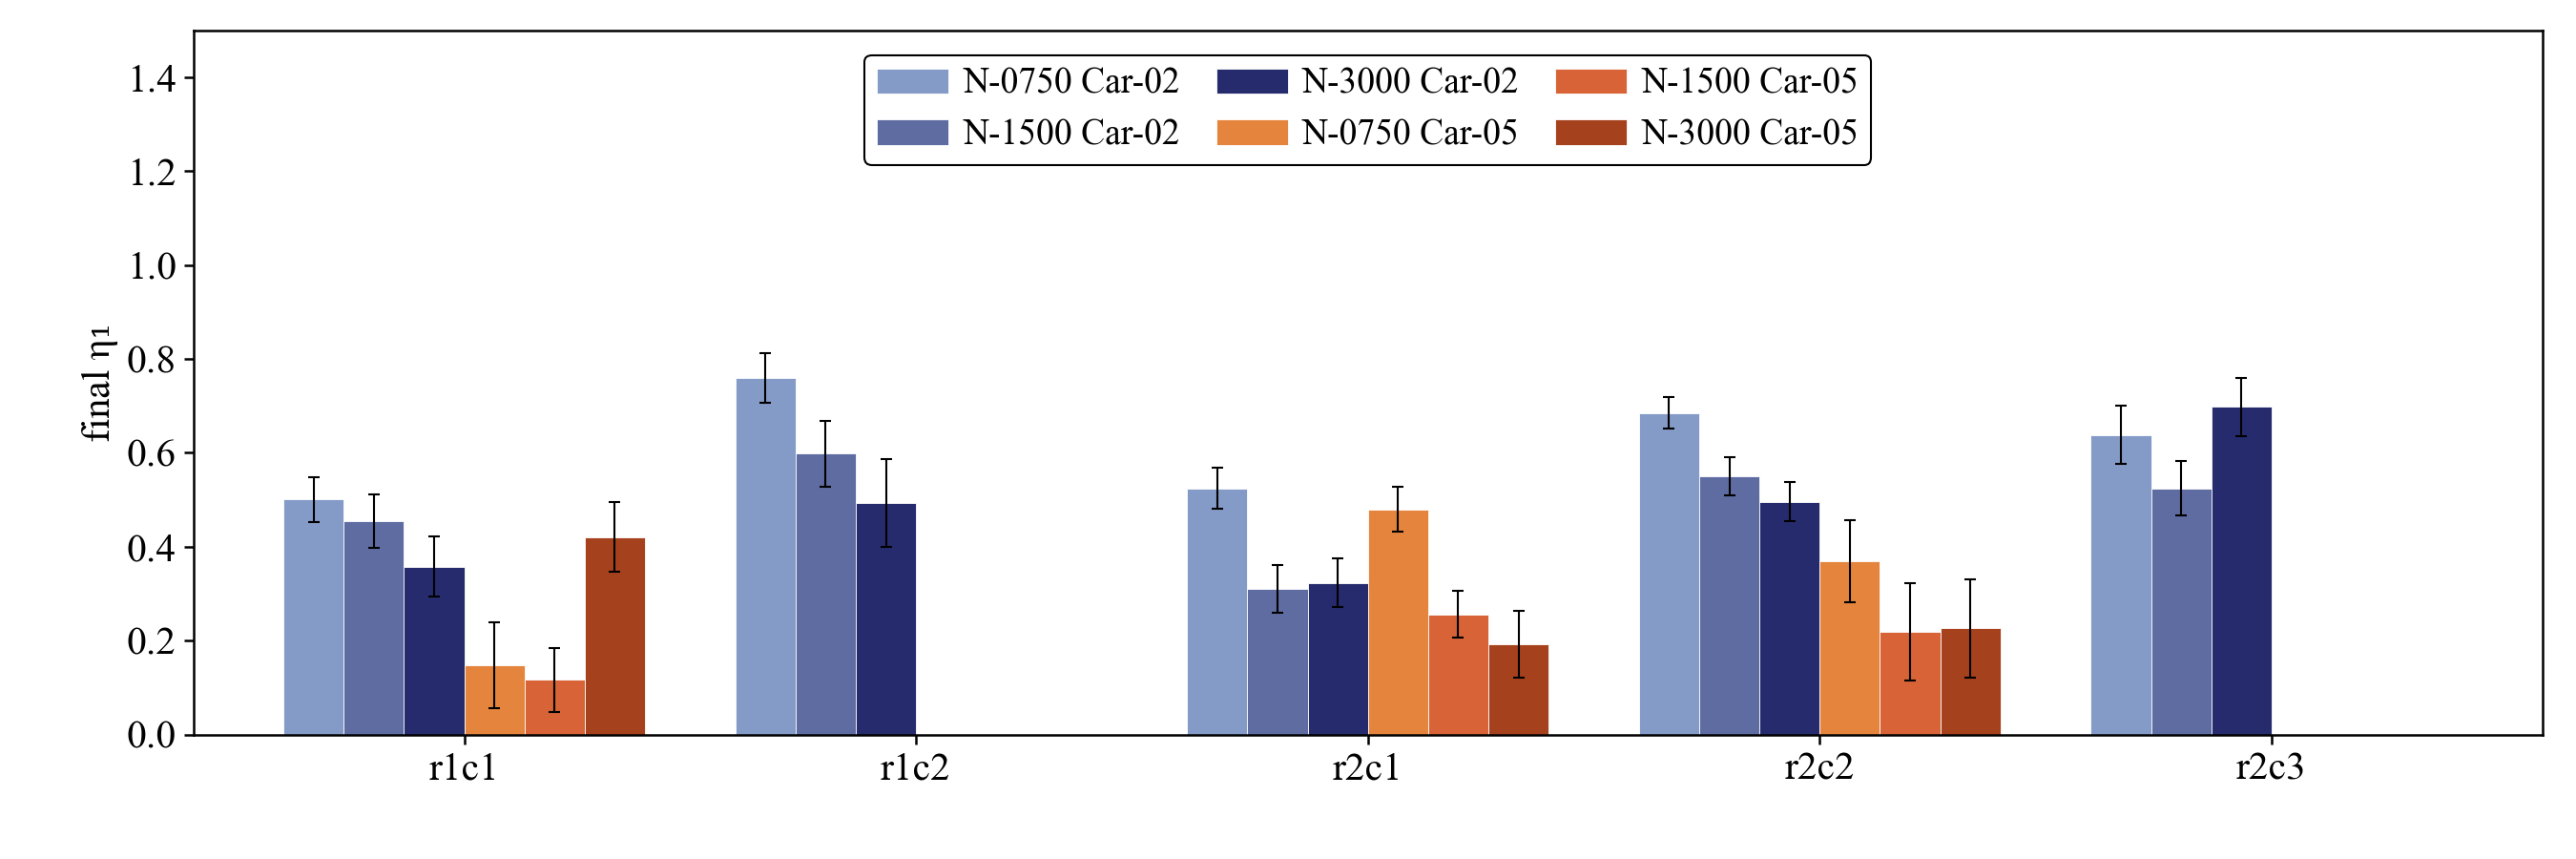
\includegraphics[width=0.9\textwidth]{Ilustraciones/A11_viga_carbopol_eta1.png}
    \caption{Caption.}
    \label{fig:cambiar}
\end{figure}

The magnitude must further be read against the dosages that produced it. The fiber contents examined here span from $0.72$ to $2.92$ times the dilute limit, barely across the threshold at which fiber-fiber interactions begin to operate and one to two orders of magnitude below the loadings of a practical mix. That the effect is small is what this regime should produce, and a small but consistent and signed effect measured at the lower edge of the semi-dilute range is a lower bound on what stronger interactions would deliver.

Taken with the previous subsection, the two mechanistic predictions of the model are confirmed in this flow. A higher fiber content raises the interaction coefficient and with it the rate of change of the orientation tensor, so the fibers reorient faster while the flow that carries them does not, which is the rotational decoupling of Section~\ref{sec:results_kinematics}. The same stronger randomizing term balances the flow at a less aligned equilibrium, so the arrested population grows more disordered with the dosage, which is the trend reported here. The models therefore apply to the unsteady, viscoplastic flow studied here, outside the Newtonian dilute setting for which they were derived, and reducing them to a compact law for this flow is warranted rather than assumed.

% ------------------------------------------------------------
\subsection{Reset of the orientation at the beam entry}
\label{sec:results_reset}
% ------------------------------------------------------------

\textcolor{blue}{Redaccion revisada}

Section~\ref{sec:framework_strain} placed the origin of the accumulated strain at the entry of the material into the beam rather than at the inlet of the mold, and the evidence for that choice is presented here. The material does not flow smoothly from the outlet into the beam. It falls and lands, and the impact against the accumulating deposit disorders the population, breaking whatever alignment the fibers carried out of the L-shape.

Figure~\ref{fig:memory_reset} follows the orientation order along the mean path against the strain accumulated from the L-shape entry. The order climbs to a peak at the last zone before the outlet and drops at the first beam cell, even though that cell sits at larger accumulated strain. A population that carried its upstream alignment across the transition would begin high and relax slowly. One that begins lower, and at the higher dosages recovers through the beam from that lower start, is a population that lands disordered and realigns within the beam.

\begin{figure}[htb]
    \centering
    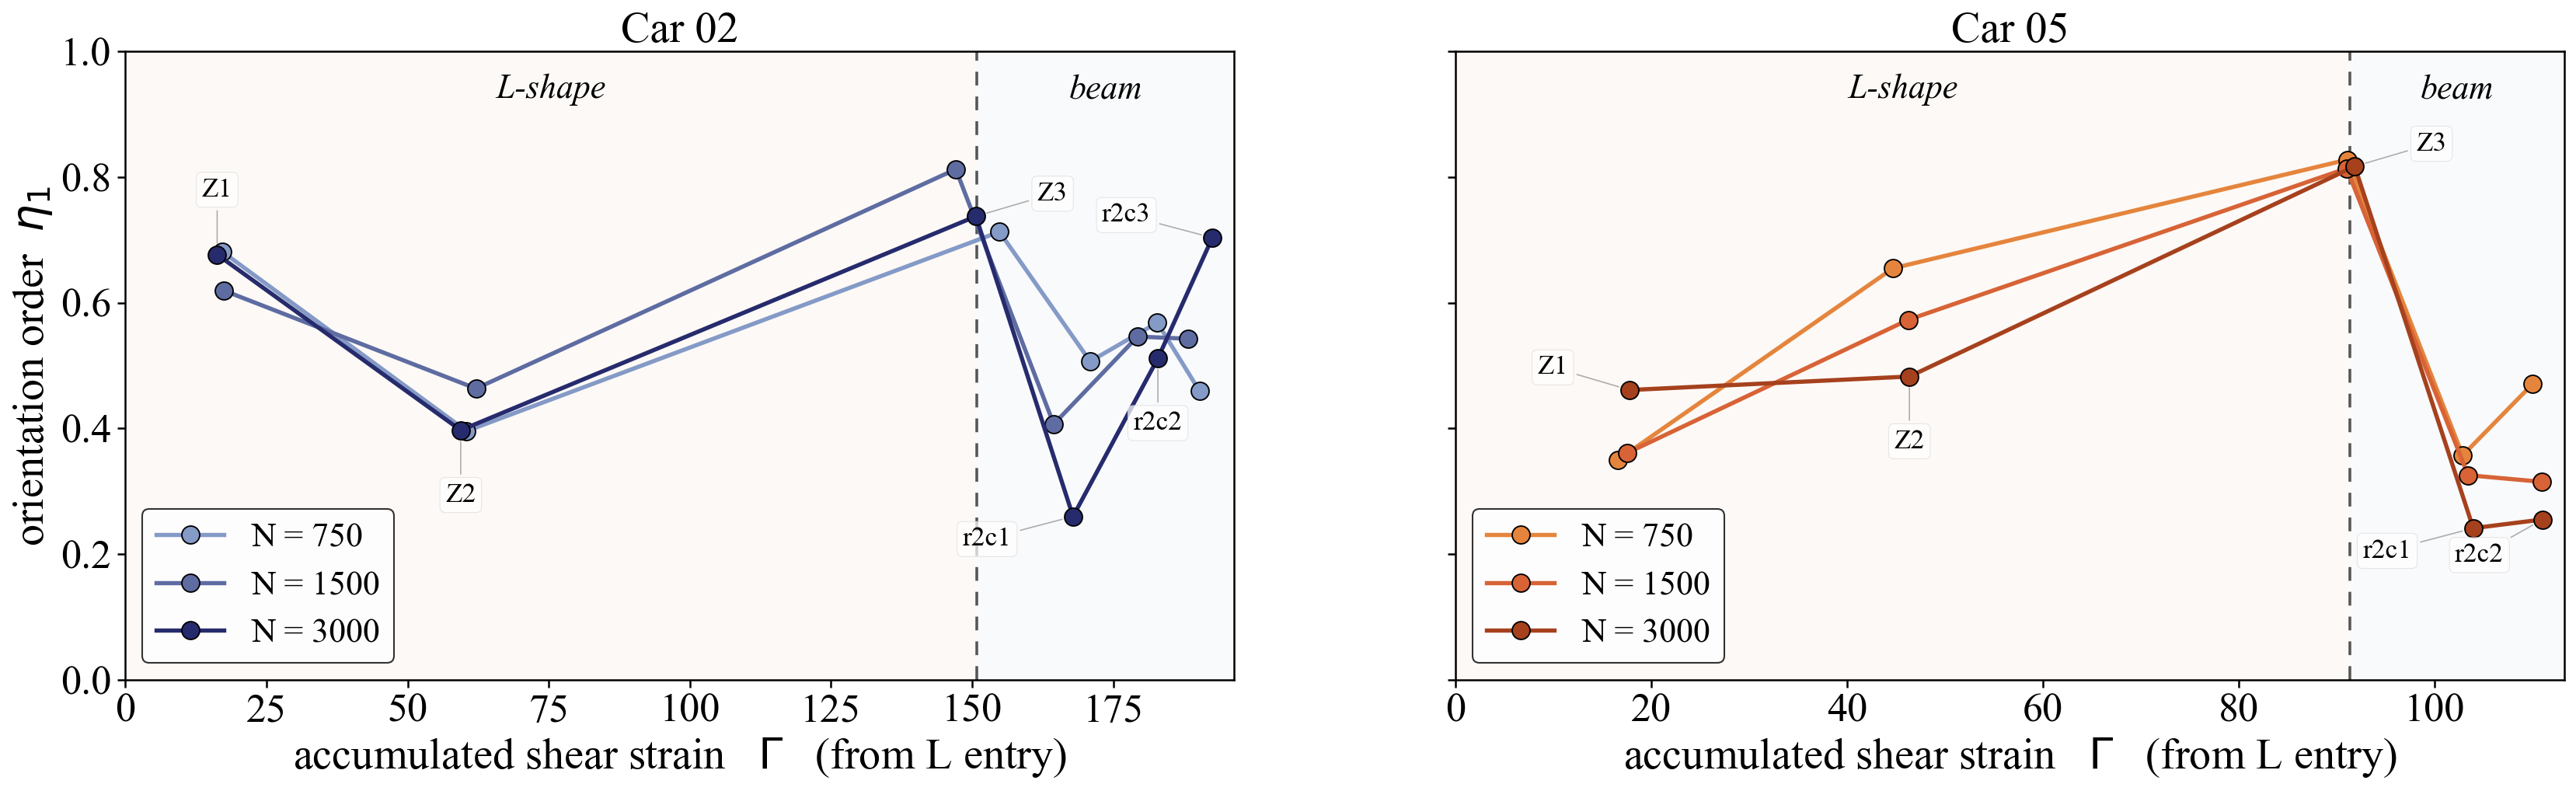
\includegraphics[width=0.9\textwidth]{Ilustraciones/fig_memoria_reset_gamma.png}
    \caption{Caption.}
    \label{fig:memory_reset}
\end{figure}

The figure supports the reset without measuring the entry order itself, and the distinction matters. The value shown for each beam cell is that of the fibers arrested there and not of the landing that precedes it, since between landing and arrest the fibers accumulate strain and regain some alignment, so the true entry state lies below the first cell and is not resolved by the measurement. The condition $\eta_{1,0}\approx 0$ adopted in Equation~\eqref{eq:saturation} is accordingly an assumption of simplicity and identifiability rather than a measured quantity: the tracking is planar while the angular state at the landing is three dimensional, and with the number of arrest points available per dosage the entry order could not be identified alongside the ceiling and the strain scale in any case.

A second consequence of the reconstructed routes bounds what follows. Only the softer matrix spans a range of accumulated strain wide enough to characterize the saturation curve, since its fibers reach five of the six beam cells and extend over the full length of the beam, so that the arrest points sample the curve from its initial rise toward saturation. The stiffer matrix arrests before the beam is filled, and its arrest points are confined to the low-strain region of the curve, where they carry no information about its shape. Together with the lower repeatability of its fiber-free baseline, this gives two independent reasons for restricting the analysis that follows to the softer formulation, so that fiber dosages are compared within a single matrix under fixed rheological and geometric conditions.

% ------------------------------------------------------------
\subsection{Fit of the saturation law}
\label{sec:results_fit}
% ------------------------------------------------------------

\textcolor{blue}{Redaccion revisada}

Fig. \ref{fig:fit_saturation_law} relates the orientation order measured in each beam cell to the shear strain accumulated by the fibers of that cell at the time of arrest, for the three dosages, together with the fit of Equation~\eqref{eq:saturation} to each. Each large marker is the arrested state of one cell, positioned by the final orientation order of its population and by the accumulated deformation at arrest, and the shaded bands are the confidence intervals of the fits.

\begin{figure}[htb]
    \centering
    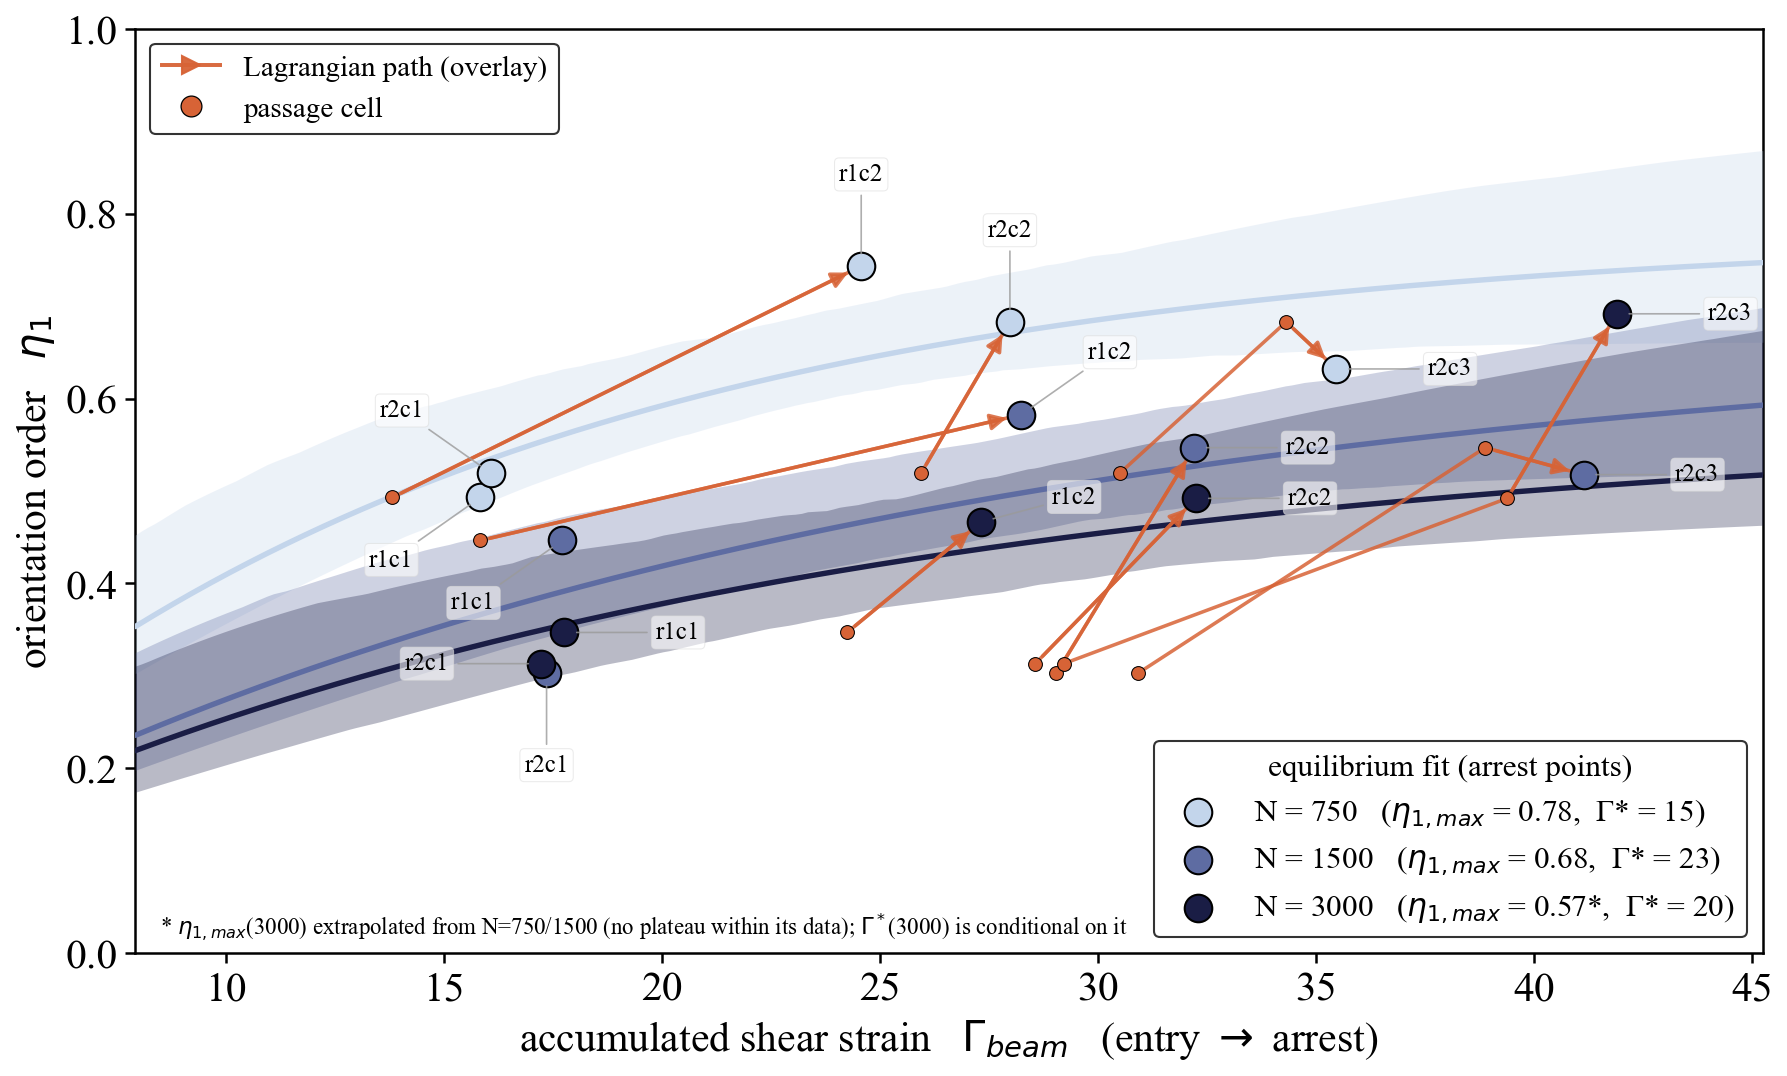
\includegraphics[width=1.0\textwidth]{Ilustraciones/fig_saturacion_trayectorias.png}
    \caption{Caption.}
    \label{fig:fit_saturation_law}
\end{figure}

Two limitations constrain what can be inferred, and both are stated before the parameters are read. The first is the number of points: each curve is fitted to five arrested cells, which is insufficient to estimate two constants with high precision, so the values reported below are initial estimates for a material of this kind rather than definitive parameters. The second concerns the cell farthest downstream. It is reached last by the advancing flow and fills least completely, its local flow is still developing against the far wall at arrest, and it is not captured in full by the camera covering it, so its arrested state is the least reliable of the five. It is retained in every figure and in the aggregate statistics, and is never used on its own to support a conclusion.

Read across the three dosages, the fits displace the equilibrium alignment in the sense the models anticipate. The ceiling falls as the fiber content rises, from $0.78$ at the lowest dosage to $0.68$ and then to $0.57$, which is the randomizing action of the fibers made visible: a denser population balances the ordering of the flow at a less aligned equilibrium. This is the central prediction of the reduction, and the measurements bear it out.

The strain scale is less straightforward. Between the two lower dosages, for which both constants are constrained by the data, it increases from $15$ to $23$: the richer suspension not only reaches a lower asymptotic alignment but also approaches it more gradually, requiring a larger accumulated deformation. At the highest dosage the strain scale cannot be determined independently, since the cells with reliable orientation measurements do not extend far enough into the high-strain regime for the population to approach its asymptote, so the ceiling is prescribed from the trend established by the two lower dosages and the strain scale is fitted conditionally on it. The only cell reaching substantially into the high-strain range is the least reliable of the five and cannot on its own constrain the asymptotic behavior, so the value reported at the highest dosage is conditional in that sense.

The increase of the strain scale with the dosage carries a meaning of its own, and it is the reading anticipated in Section~\ref{sec:governing}. Because the two constants share the denominator $(a+b)$, interactions acting only by raising the randomizing rate $b$ would lower the ceiling and lower the strain scale together, so that a richer suspension would align less but saturate sooner. That the strain scale instead rises indicates that the interactions also degrade the effective ordering rate $a$ supplied by the flow, retarding the alignment in addition to opposing it, which is the slow-kinetics behavior documented for concentrated fiber suspensions [CITAR].

Expressed in angular form through Equation~\eqref{eq:angle_predictor}, the same fits reveal the asymptotic angular deviation, which widens with the fiber content from $19.3^\circ$ to $24.0^\circ$ and then to $27.7^\circ$, the last value conditional in the same sense as the ceiling from which it derives. The change of variable introduces no additional fitting freedom, since the strain scale is carried over unchanged. Because the principal direction of deformation is nearly horizontal in this region, a larger asymptotic deviation corresponds to a broader angular distribution about the preferred flow direction, and the decrease in equilibrium alignment is recovered in equivalent form as an increase in residual angular dispersion.

\textcolor{red}{HAY QUE LLAMAR A LA FIGURA}

\begin{figure}[htb]
    \centering
    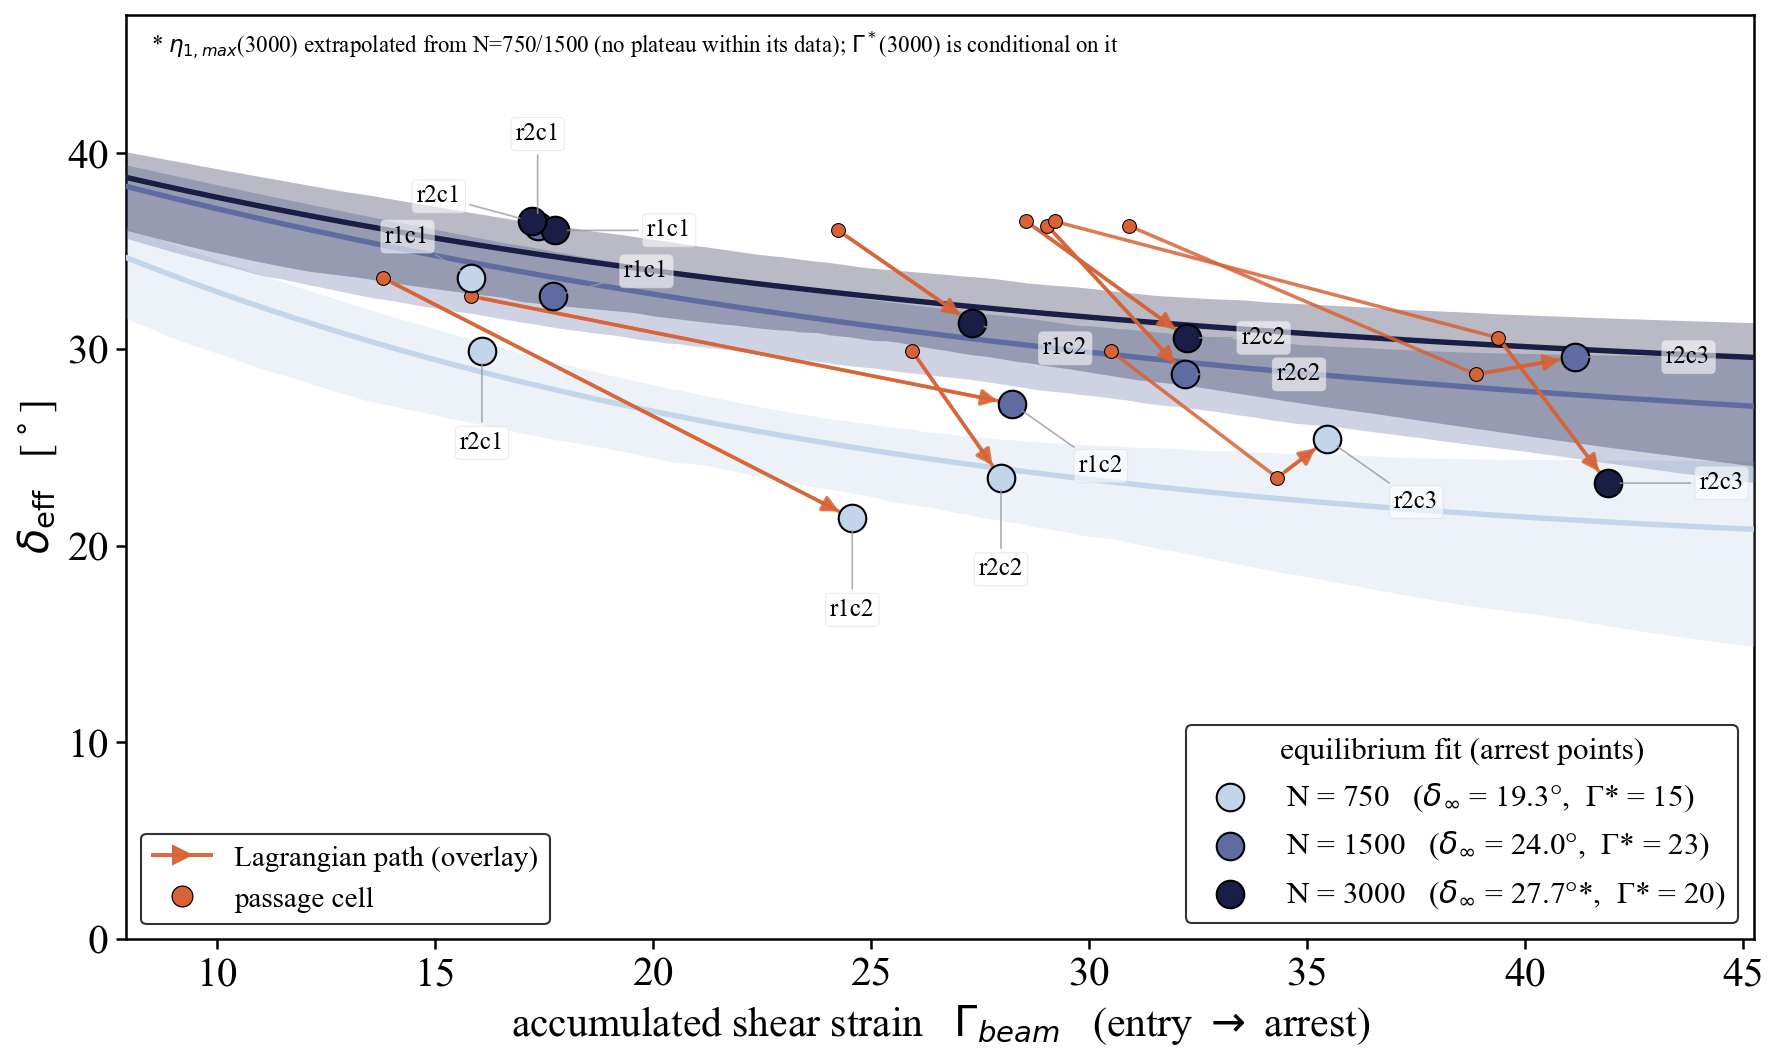
\includegraphics[width=1.0\textwidth]{Ilustraciones/M4_ley_angular_viga.png}
    \caption{Caption.}
    \label{fig:fit_saturation_law_angle}
\end{figure}

% ------------------------------------------------------------
\subsection{Prediction from the fiber-free flow}
\label{sec:results_prediction}
% ------------------------------------------------------------

\textcolor{blue}{Redaccion revisada}

The fits of the previous subsection use the strain accumulated by the fiber-laden suspensions themselves, and are therefore a calibration rather than a test. The test reverses the procedure. For each cell of the beam, the strain accumulated over the full duration of the casting is computed from the PIV of the fiber-free flow, the corresponding angle is obtained from the calibrated predictor of Equation~\eqref{eq:angle_predictor}, and it is compared with the angle measured for the fiber population arrested in that same cell. The asymmetry that makes the test possible is that the deformation a fiber accumulates can be read from the flow before any fibers are added, whereas its alignment can only be read from the fibers themselves.

\textcolor{red}{HAY QUE LLAMAR A LA FIGURA}

\begin{figure}[htb]
    \centering
    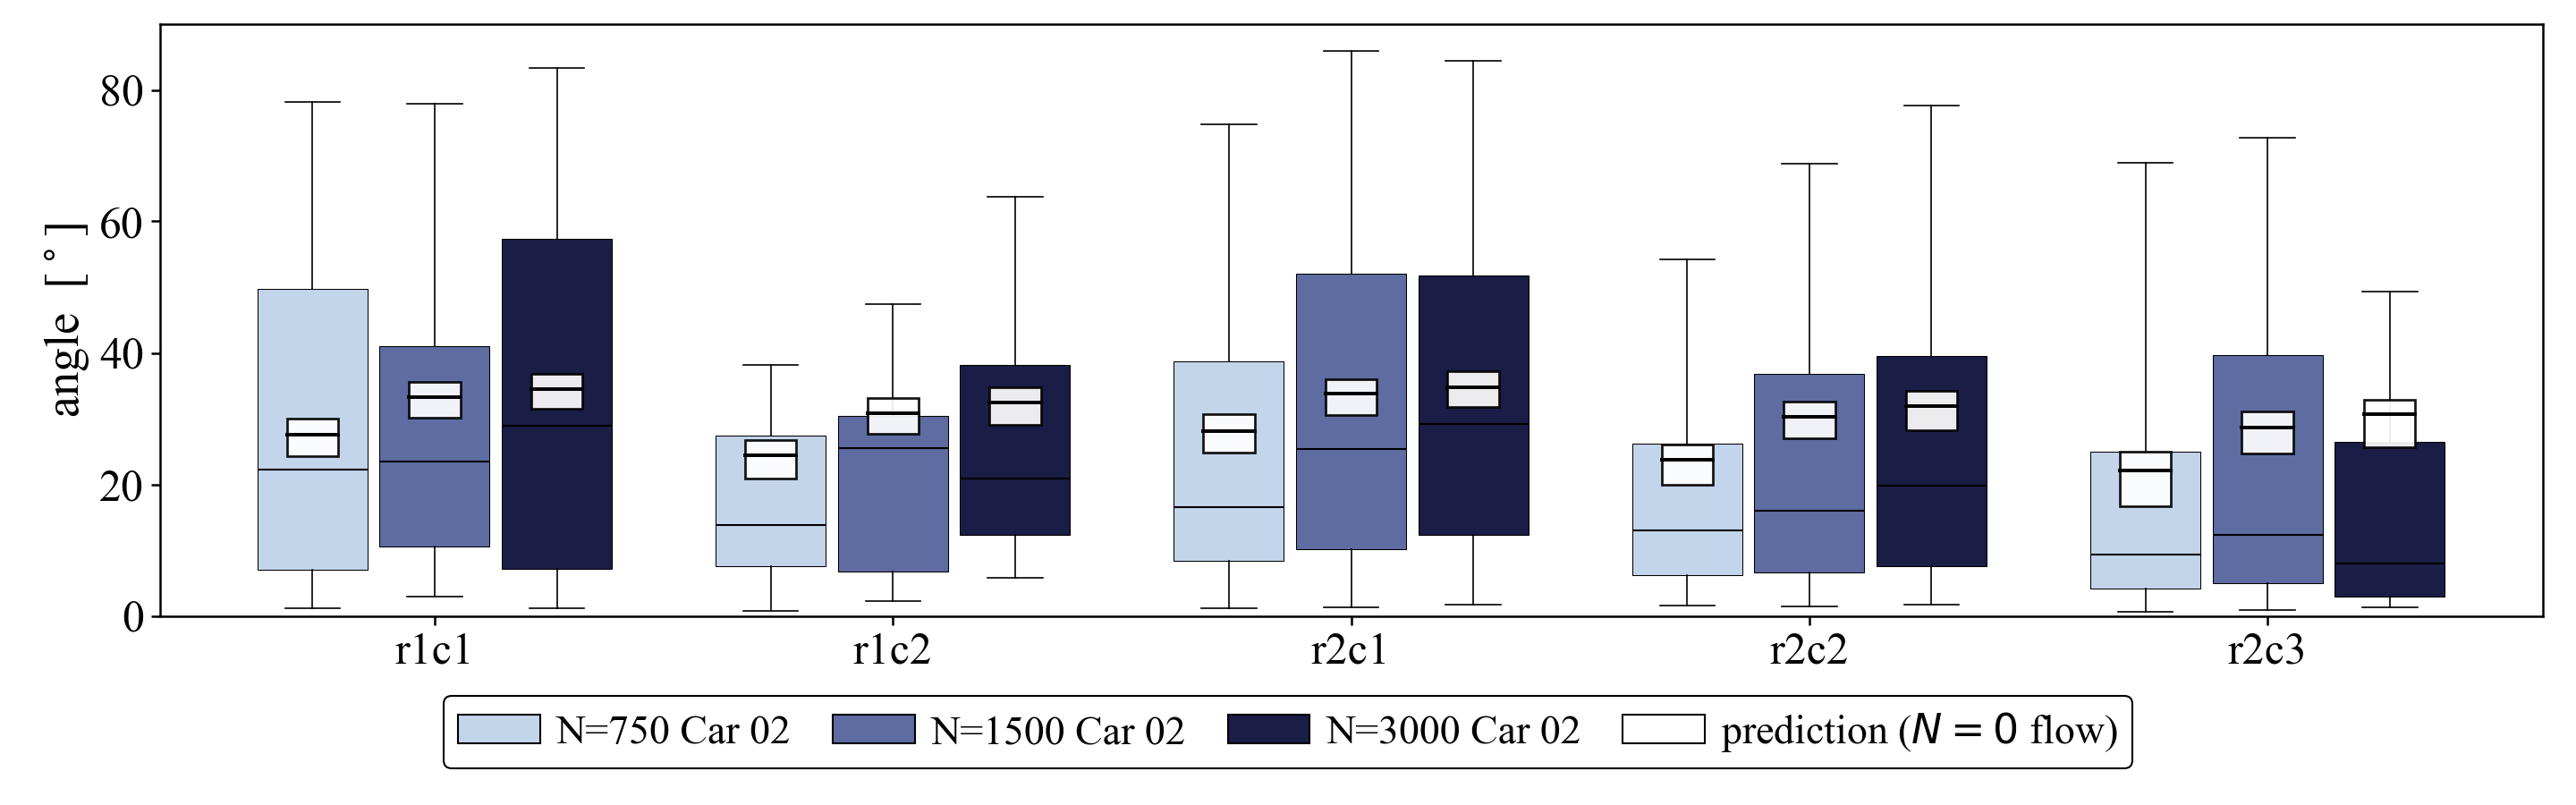
\includegraphics[width=1.0\textwidth]{Ilustraciones/M5_val_ang_fibra_box.png}
    \caption{Caption.}
    \label{fig:fit_saturation_law}
\end{figure}

Across the three dosages the predictions remain within the tolerance of $\pm 5^\circ$ adopted here. The mean signed departure stays below $2^\circ$ at every dosage, the root-mean-square departure does not exceed $3.7^\circ$, and none of the three dosages exhibits a bias statistically distinguishable from zero. The agreement holds over the full range examined, from the dilute regime at the lowest dosage to the lower part of the semi-dilute regime at the highest, and shows no systematic deterioration as the concentration increases.

\textcolor{red}{HAY QUE LLAMAR A LA TABLA}

\begin{table}[htb]
\centering
\caption{Agreement between the predicted and the measured final angle, by fiber dosage, over all beam cells. The prediction uses the accumulated strain of the fiber-free flow. The bias is the mean signed departure, the RMSE its root-mean-square, and $p$ tests the bias against zero; the practical tolerance is $\pm5^\circ$.}
\label{tab:angle_test}
\begin{tabular}{lcccc}
\toprule
$N$ [fibers] & regime & bias [$^\circ$] & RMSE [$^\circ$] & $p$ \\
\midrule
750  & dilute      & $+1.3$ & $3.5$ & $0.46$ \\
1500 & semi-dilute & $-0.7$ & $2.3$ & $0.56$ \\
3000 & semi-dilute & $-1.7$ & $3.7$ & $0.37$ \\
\bottomrule
\end{tabular}
\end{table}

The cell farthest downstream is retained in these statistics, and it is among the cells for which the agreement is least favorable, particularly at the highest dosage, which is consistent with it being the least reliably observed of the five. Excluding it improves the aggregate agreement without changing the conclusion: the bias remains small and indistinguishable from zero, and the root-mean-square departure remains within the tolerance, at every dosage and with the cell either retained or removed.

The result carries a consequence beyond the validation of the predictor. That the deformation field of the fiber-free flow serves as input without introducing a systematic error indicates that, over the concentration range examined, the modification the fibers impose on the deformation field remains small enough for the unladen flow to stand in for the laden one. Section~\ref{sec:results_kinematics} showed that the fibers do perturb the carrier, and regionally by a large amount; what this test establishes is that the perturbation does not propagate into the accumulated strain in a way that corrupts the orientation predicted from it. Within this range, a one-way coupling suffices to predict the final orientation of the population.

\section{Discussion / Conclusions}







% ── Bibliography ─────────────────────────────────────────────
\section*{REFERENCES}
\bibliography{references}

% ── Figures ──────────────────────────────────────────────────
\end{document}
